\documentclass[9pt, landscape, a4paper]{article}

\usepackage{fontspec}
\renewcommand{\normalsize}{\fontsize{9}{11}\selectfont}
\usepackage[english]{babel}
\babelfont{rm}{Noto Sans}
\babelfont{sf}{Noto Sans}

\usepackage{amsmath}
\usepackage{amssymb}
\usepackage{hyperref}
\usepackage{url}
\usepackage{graphicx}
\usepackage{geometry}
\usepackage{enumitem}
\usepackage{parskip}
\usepackage{chemfig}
\usepackage{pdfpages}
\usepackage{xcolor}
\usepackage{tikz}
\usepackage{fancybox}
\usepackage{makecell}
\usepackage{pgfplots}
\usepackage{ulem}
\usepackage{wrapfig}
\usepackage{subcaption}
\usepackage{esvect}
\usepackage{siunitx}
\usepackage{mathtools}
\usepackage{varwidth}
\usepackage{multicol}
\usepackage{titlesec}
\usepackage{bm}
\usepackage{forest}
\usepackage{upgreek}
\usepackage{tabularx}

\usetikzlibrary{arrows, arrows.meta}
\usetikzlibrary{decorations.pathreplacing}
\usetikzlibrary{patterns}
\usetikzlibrary{shapes.geometric}
\pgfplotsset{compat=1.18}
\definecolor{darkgreen}{rgb}{0.0, 0.6, 0.0}
\DeclareMathOperator\arctanh{arctanh}

% ============= GEOMETRY =============
\geometry{
    a4paper,
    landscape,
    left=0.5cm,
    right=0.5cm,
    top=1.5cm, 
    bottom=0.5cm,
    footskip=0cm
}

\setlist{nosep, leftmargin=*}

\AtBeginDocument{
  \setlength{\abovedisplayskip}{3pt}
  \setlength{\belowdisplayskip}{3pt}
  \setlength{\abovedisplayshortskip}{0pt}
  \setlength{\belowdisplayshortskip}{0pt}
}

% ============= HEADER & TITLES =============
\usepackage{fancyhdr}
\pagestyle{fancy}
\fancyhf{}
\rhead{\small \vspace*{.1cm}Applied Process Control Cheatsheet}
\lhead{\small \vspace*{.1cm}Matteo Frongillo}
\cfoot{\small \vspace*{.4cm}\thepage}
\newcommand{\TotalPages}{10}
\cfoot{\small \vspace*{.4cm}\thepage/\TotalPages}
\renewcommand{\headrulewidth}{0pt}
\setlength{\headsep}{4pt}

\titlespacing*{\part}{0pt}{6pt}{1pt}
\titlespacing*{\section}{0pt}{6pt}{1pt}
\titlespacing*{\subsection}{0pt}{6pt}{1pt}
\titlespacing*{\subsubsection}{0pt}{6pt}{1pt}

\titleformat{\part}{\large\bfseries\color{black}}{\thepart.}{0.4em}{}
\titleformat{\section}{\normalsize\bfseries\color{red!80}}{}{0em}{}
\titleformat{\subsection}{\small\bfseries\color[HTML]{007AFF}}{}{0em}{}
\titleformat{\subsubsection}{\small\bfseries\color[HTML]{007355}}{}{0em}{}

% ============= META DATA =============
\newcommand{\pdftitle}[1]{\hypersetup{
  colorlinks=true,
  linkcolor=black,
  urlcolor=blue,
  pdftitle={#1},
  pdfauthor={Matteo Frongillo}
}}

% ============= RENEW COMMANDS =============

\makeatletter
\renewcommand{\author}[1]{%
  \def\@author{%
    #1\\
    \parbox{\textwidth}{%
      \centering
      \small Last update: \today
    }
  }%
}
\makeatother

\let\emptyset\varnothing

\makeatletter
\pgfmathdeclarefunction{arctan}{1}{%
    \begingroup
    \pgfmathparse{rad(atan(#1))}%
    \endgroup
}
\makeatother

\renewcommand{\tau}{\uptau}
\renewcommand{\nu}{\upnu}

% ============= NEW COMMANDS =============

\newcommand{\figbox}[1]{ 
  \begin{center}
    \fbox{\begin{varwidth}{\textwidth} #1 \end{varwidth}} 
  \end{center}       
}

\newcommand{\wrapfill}{
    \par
    \ifnum \value{WF@wrappedlines} > 0
        \addtocounter{WF@wrappedlines}{-1}%
        \null\vspace{
            \arabic{WF@wrappedlines}
            \baselineskip
        }
        \WFclear
    \fi
    \phantom{}
}

\ExplSyntaxOn
\DeclareDocumentCommand{\integral}{d[] d[] d[] d[]}
{
    \IfNoValueTF{#3}{
        \IfNoValueTF{#4}{
            \displaystyle \int #1\,d#2
        }{
            \text{Error: either 2 or 4 arguments must be provided}
        }
    }{
        \IfNoValueTF{#4}{
            \text{Error: either 2 or 4 arguments must be provided}
        }{
            \displaystyle
            \int\limits
                \IfNoValueF{#1}{\c_math_subscript_token{#1}}
                ^{\IfNoValueTF{#2}{}{#2}}
                #3\, d#4
        }
    }
}
\ExplSyntaxOff

\newcommand*\circled[1]{\tikz[baseline=(char.base)]{
            \node[shape=circle,draw,inner sep=1pt] (char) {\small #1};}}

\makeatletter
\newcommand*{\rom}[1]{\expandafter\@slowromancap\romannumeral #1@}
\makeatother

\makeatletter
\newcommand{\shorteq}{\mathrel{\mkern0.2mu\mathpalette\shorteq@\relax\mkern0.2mu}}
\newcommand{\shorteq@}[2]{\scalebox{0.5}[1]{$\m@th#1=$}}

\newcommand{\longeq}[1]{\mathrel{\mathpalette\longeq@{#1}}}
\newcommand{\longeq@}[2]{%
  \begingroup
  \sbox\z@{$\m@th#1=$}%
  \ifdim#2<\wd\z@
    \resizebox{#2}{\height}{\box\z@}%
  \else
    \ifdim#2<3\wd\z@
      \hbox to #2{$\m@th#1=\hss=\hss=\hss=$}%
    \else
      \hbox to #2{$\m@th#1=\cleaders\hbox to 0.2\wd\z@{\hss$#1=$\hss}\hfil=$}%
    \fi
  \fi
  \endgroup
}
\makeatother

\newcommand{\const}{%
  \ \mathrel{\ooalign{%
    \hfil$c$\hfil\cr
    \hfil\kern0.10em\raisebox{-0.4ex}{\rule{0.08pt}{1.7ex}}\hfil\cr
  }}%
}

\makeatletter
\define@key{Gin}{lw}[1]{\setkeys{Gin}{width=#1\linewidth}}
\newcommand{\lw}{lw}
\makeatother

\newcommand{\difference}{\,\backslash\,}
\newcommand{\rem}{\underline{Remark}: }
\newcommand{\nots}{\underline{Notation}: }
\newcommand{\note}{\underline{Note}: }
\newcommand{\prf}{\underline{Proof}: }
\newcommand{\exs}{\underline{Example}: }
\newcommand{\defs}{\underline{Definition}: }
\newcommand{\wrn}{\underline{Warning}: }
\newcommand{\sht}{\ |\ }
\newcommand{\pph}[1]{\paragraph{#1} \phantom{}\\}
\newcommand{\dm}{\displaystyle}
\newcommand{\rad}{^{\mathrm{c}}}
\newcommand{\dsum}[2]{\displaystyle \sum_{#1}^{#2}}
\newcommand{\dx}[2]{\dfrac{{\mathrm{d}}^{#1}{#2}}{\mathrm{d}x^{#1}}}
\newcommand{\der}[2]{\dfrac{{\mathrm{d}}{#1}}{\mathrm{d}{#2}}}
\newcommand{\cel}{$^\circ$C}

% ============= DOCUMENT CONTENT =============

\begin{document}
\pdftitle{Applied Process Control}
\vspace*{-.5cm}
\setlength{\columnsep}{0.5cm}

\begin{multicols*}{3}
\raggedcolumns
\vspace*{-.7cm}
\part{Control Theroy and Automation}
A control system regulates a process using sensors, controllers, actuators, and feedback.

Control theory designs controllers to regulate and optimize dynamic systems.

\section{Uncontrolled system}
\begin{center}
    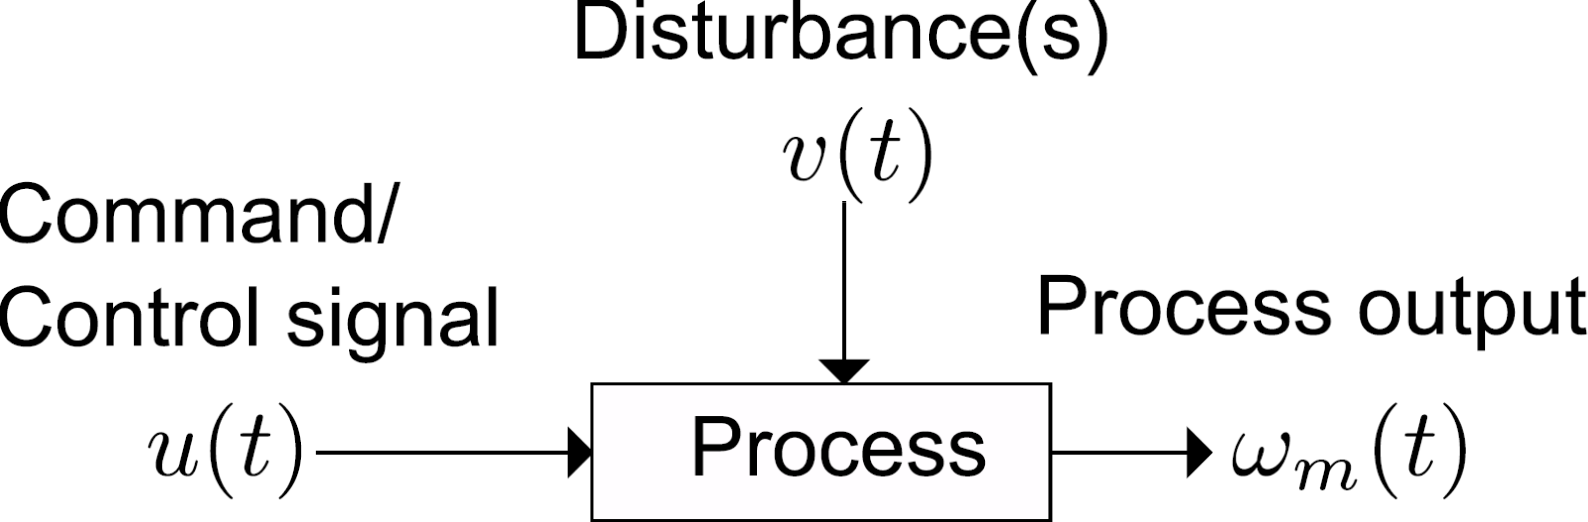
\includegraphics[width=.8\linewidth]{media-cheatsheet/uncontrolled.png}
\end{center}

\section{Open-loop controlled system}
\begin{center}
    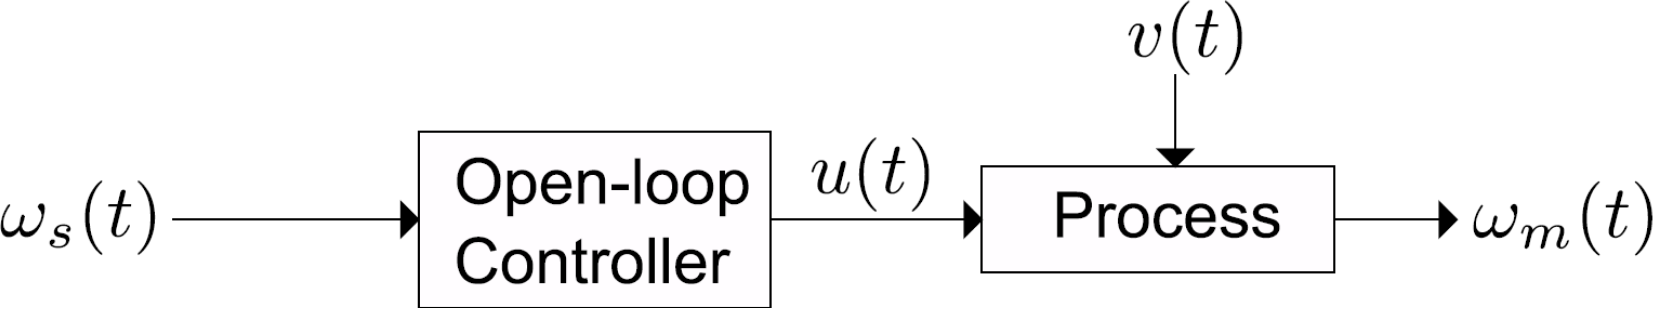
\includegraphics[width=\linewidth]{media-cheatsheet/openloop.png}
\end{center}

\subsection{Advantages}
\begin{itemize}
    \item Simple structure: no sensors or controllers needed
    \item Low cost: fewer components and less complexity
\end{itemize}

\subsection{Disadvantages}
\begin{itemize}
    \item No adaptation: cannot correct changes or disturbances
    \item Unstable performance: quality may decrease over time
\end{itemize}

\section{Closed-loop controlled system}
\begin{center}
    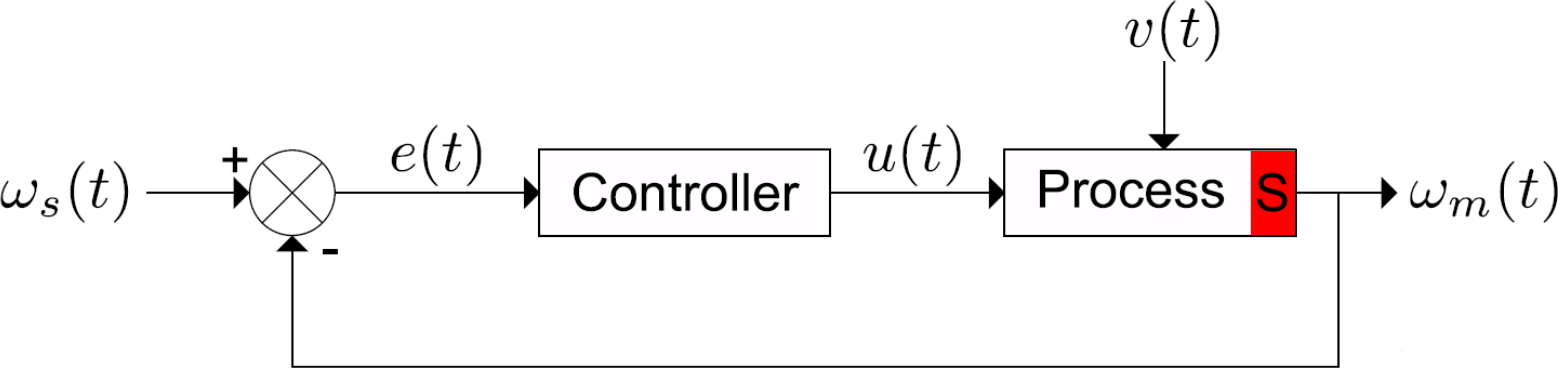
\includegraphics[width=\linewidth]{media-cheatsheet/closedloop.png}
\end{center}

\subsection{Advantages}
\begin{itemize}
    \item High accuracy: continuous correction improves precision, performance, and efficiency
    \item Adaptation: reacts to load changes, disturbances, or operating conditions
\end{itemize}

\subsection{Disadvantages}
\begin{itemize}
    \item Complex structure: sensors, controllers, and feedback are required
    \item Higher cost: more components increase total cost
    \item More maintenance: components need calibration and maintenance
\end{itemize}

\newcolumn
\section{Extended block diagram}
\begin{center}
    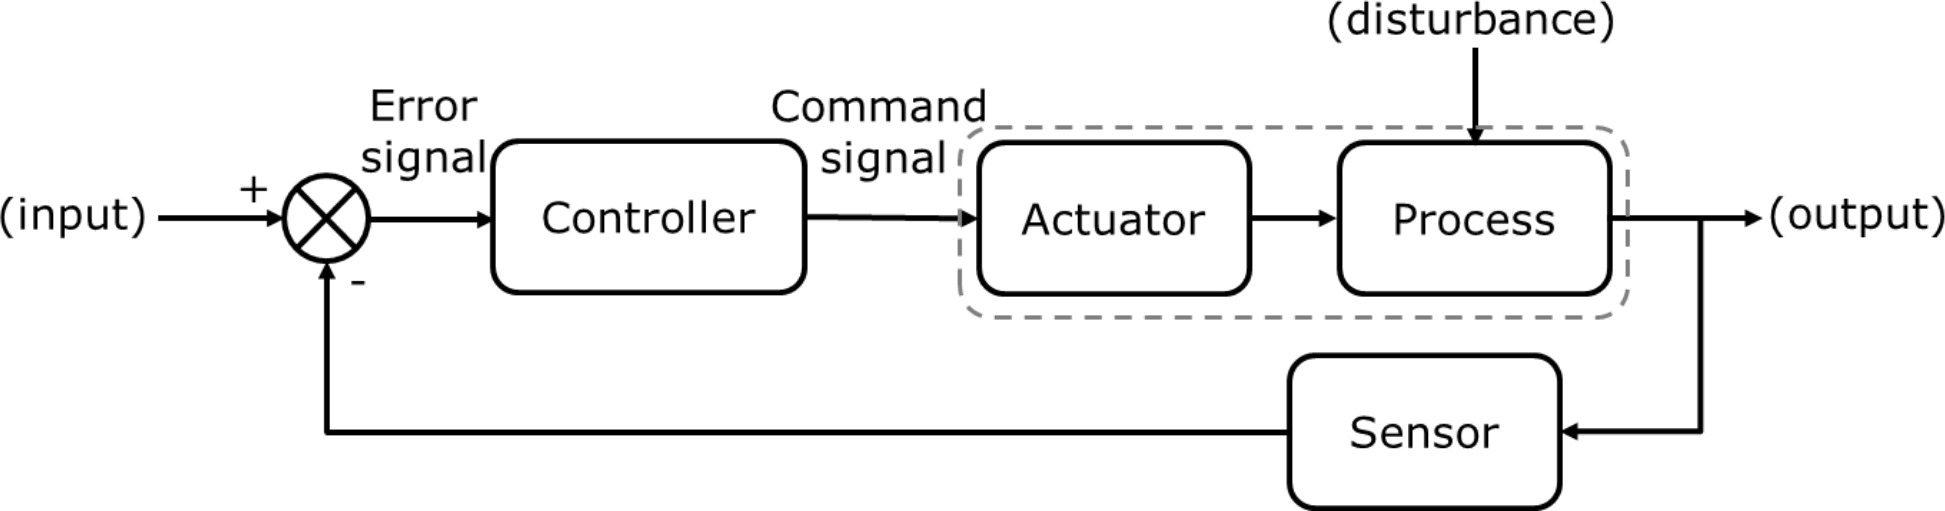
\includegraphics[width=\linewidth]{media-cheatsheet/extended.png}
\end{center}
\vspace*{-.2cm}
\subsection{Components}
\begin{minipage}[t]{0.48\linewidth}
    \subsubsection{Controller}
    Input: error $e(t)$\\
    Output: command signal $u(t)$
\end{minipage}
\hfill
\begin{minipage}[t]{0.48\linewidth}
    \subsubsection{Actuator}
    Input: command signal $u(t)$\\
    Output: process input signal
\end{minipage}

\subsubsection{Process}
Input: process input signal\\
Unwanted output: disturbance/noise $v(t)$\\
Output: actual process output $y_m(t)$

\subsubsection{Sensor}
Input: actual process output $y_m(t)$\\
Output: signal to be compared to the desired output signal

\section{Feedback loop in a closed-loop control}
\begin{center}
    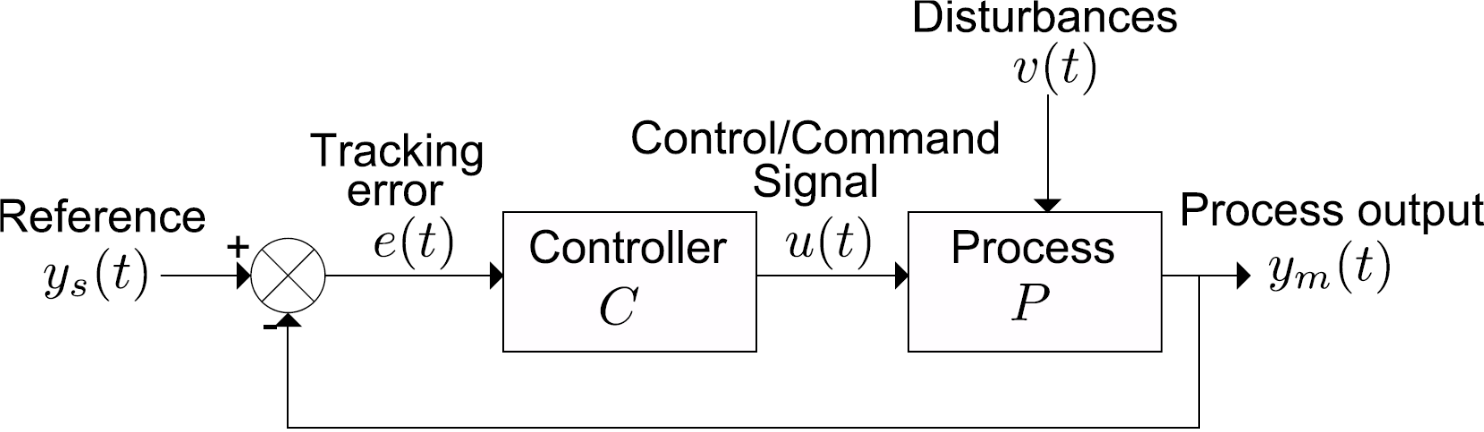
\includegraphics[width=\linewidth]{media-cheatsheet/feedback.png}
\end{center}
\vspace*{-.5cm}
\begin{minipage}[t]{0.48\linewidth}
    \begin{align*}
        &e(t) = y_s(t) - y_m(t)\\
        &u(t) = C(e(t))\\
        &y_m(t) = P(u(t),v(t))
    \end{align*}
\end{minipage}
\hfill
\begin{minipage}[t]{0.48\linewidth}
    \begin{align*}
        &y_s(t), e(t), u(t), y_m(t):\ \text{Signals}\\
        &P, C:\ \text{Systems}
    \end{align*}
\end{minipage}

\subsection{Signals vs System}
\subsubsection{Signals}
\begin{itemize}
    \item Carry information through variations in a physical quantity
    \item Described as functions of one or more variables
    \item Can be natural or artificial and are used in communication, measurement, and control
\end{itemize}

\subsubsection{System}
\begin{itemize}
    \item Interconnection of components used to perform a specific function
    \item Takes input signals, processes or transforms them, and produces output signals
    \item Describes the relationship between inputs and outputs
\end{itemize}

\section{Automation pyramid}
\begin{enumerate}[label=Level \arabic*., start=0]
    \item Field/process level
    \item Control devices level
    \item Supervisory control level
    \item Manufacturing planning and execution system (MES)
    \item Management/Business level or ERP
    \item Digital transformation and AI-driven intelligent ecosystems (cloud level)
\end{enumerate}

\subsection{Control engineering}
Levels 0-1: real-time control of physical processes using sensors, measurement systems, actuators, and controllers

\subsection{Automation}
Levels 2-5: integration, supervision, optimization, planning, and management of production and business processes

\part{Good controllers}
\section{Sauna example, closed-loop control}
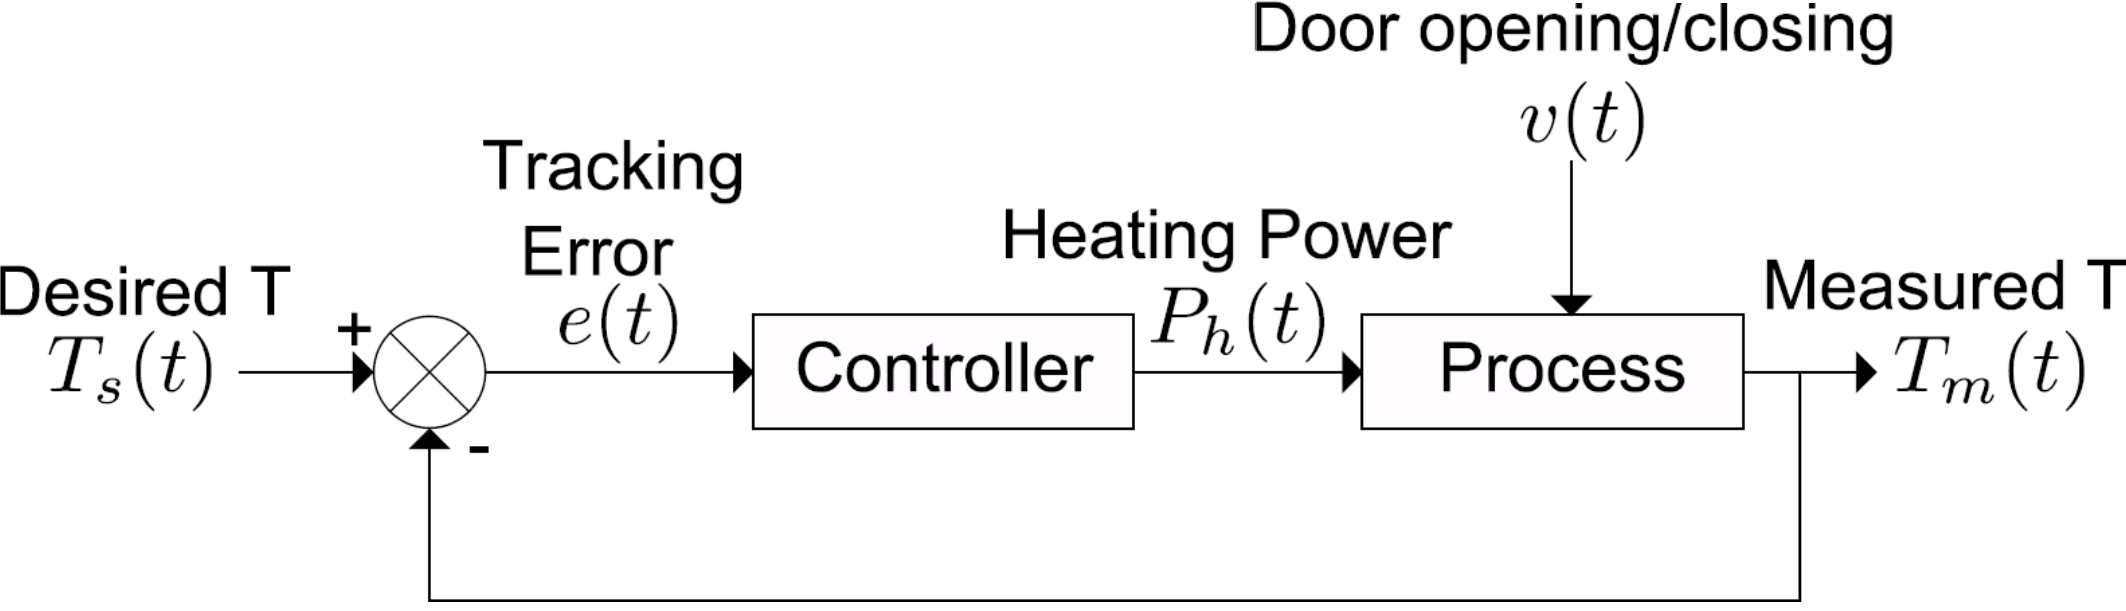
\includegraphics[\lw]{media-cheatsheet/sauna.png}

\subsection{Disturbance rejection}
\begin{itemize}
    \item Ability to reduce the effect of internal or external disturbances on the system output
    \item Keeps the output close to the desired reference
\end{itemize}

\subsubsection{Characteristics}
\begin{itemize}
    \item Disturbance types: internal component changes or external environmental changes
    \item Effectiveness: controller detects and compensates disturbances
    \item Control strategies: feedback control reacts after disturbance; feedforward control acts before it affects the output
\end{itemize}

\subsubsection{Performance metrics}
\begin{itemize}
    \item Stability: system remains robust under disturbances
    \item Steady-state error: final deviation from the reference is minimized
    \item Overshoot/undershoot: excessive output deviations are reduced
    \item Rise/settling time: response is fast and stable
\end{itemize}

\subsubsection{Graphical representation}
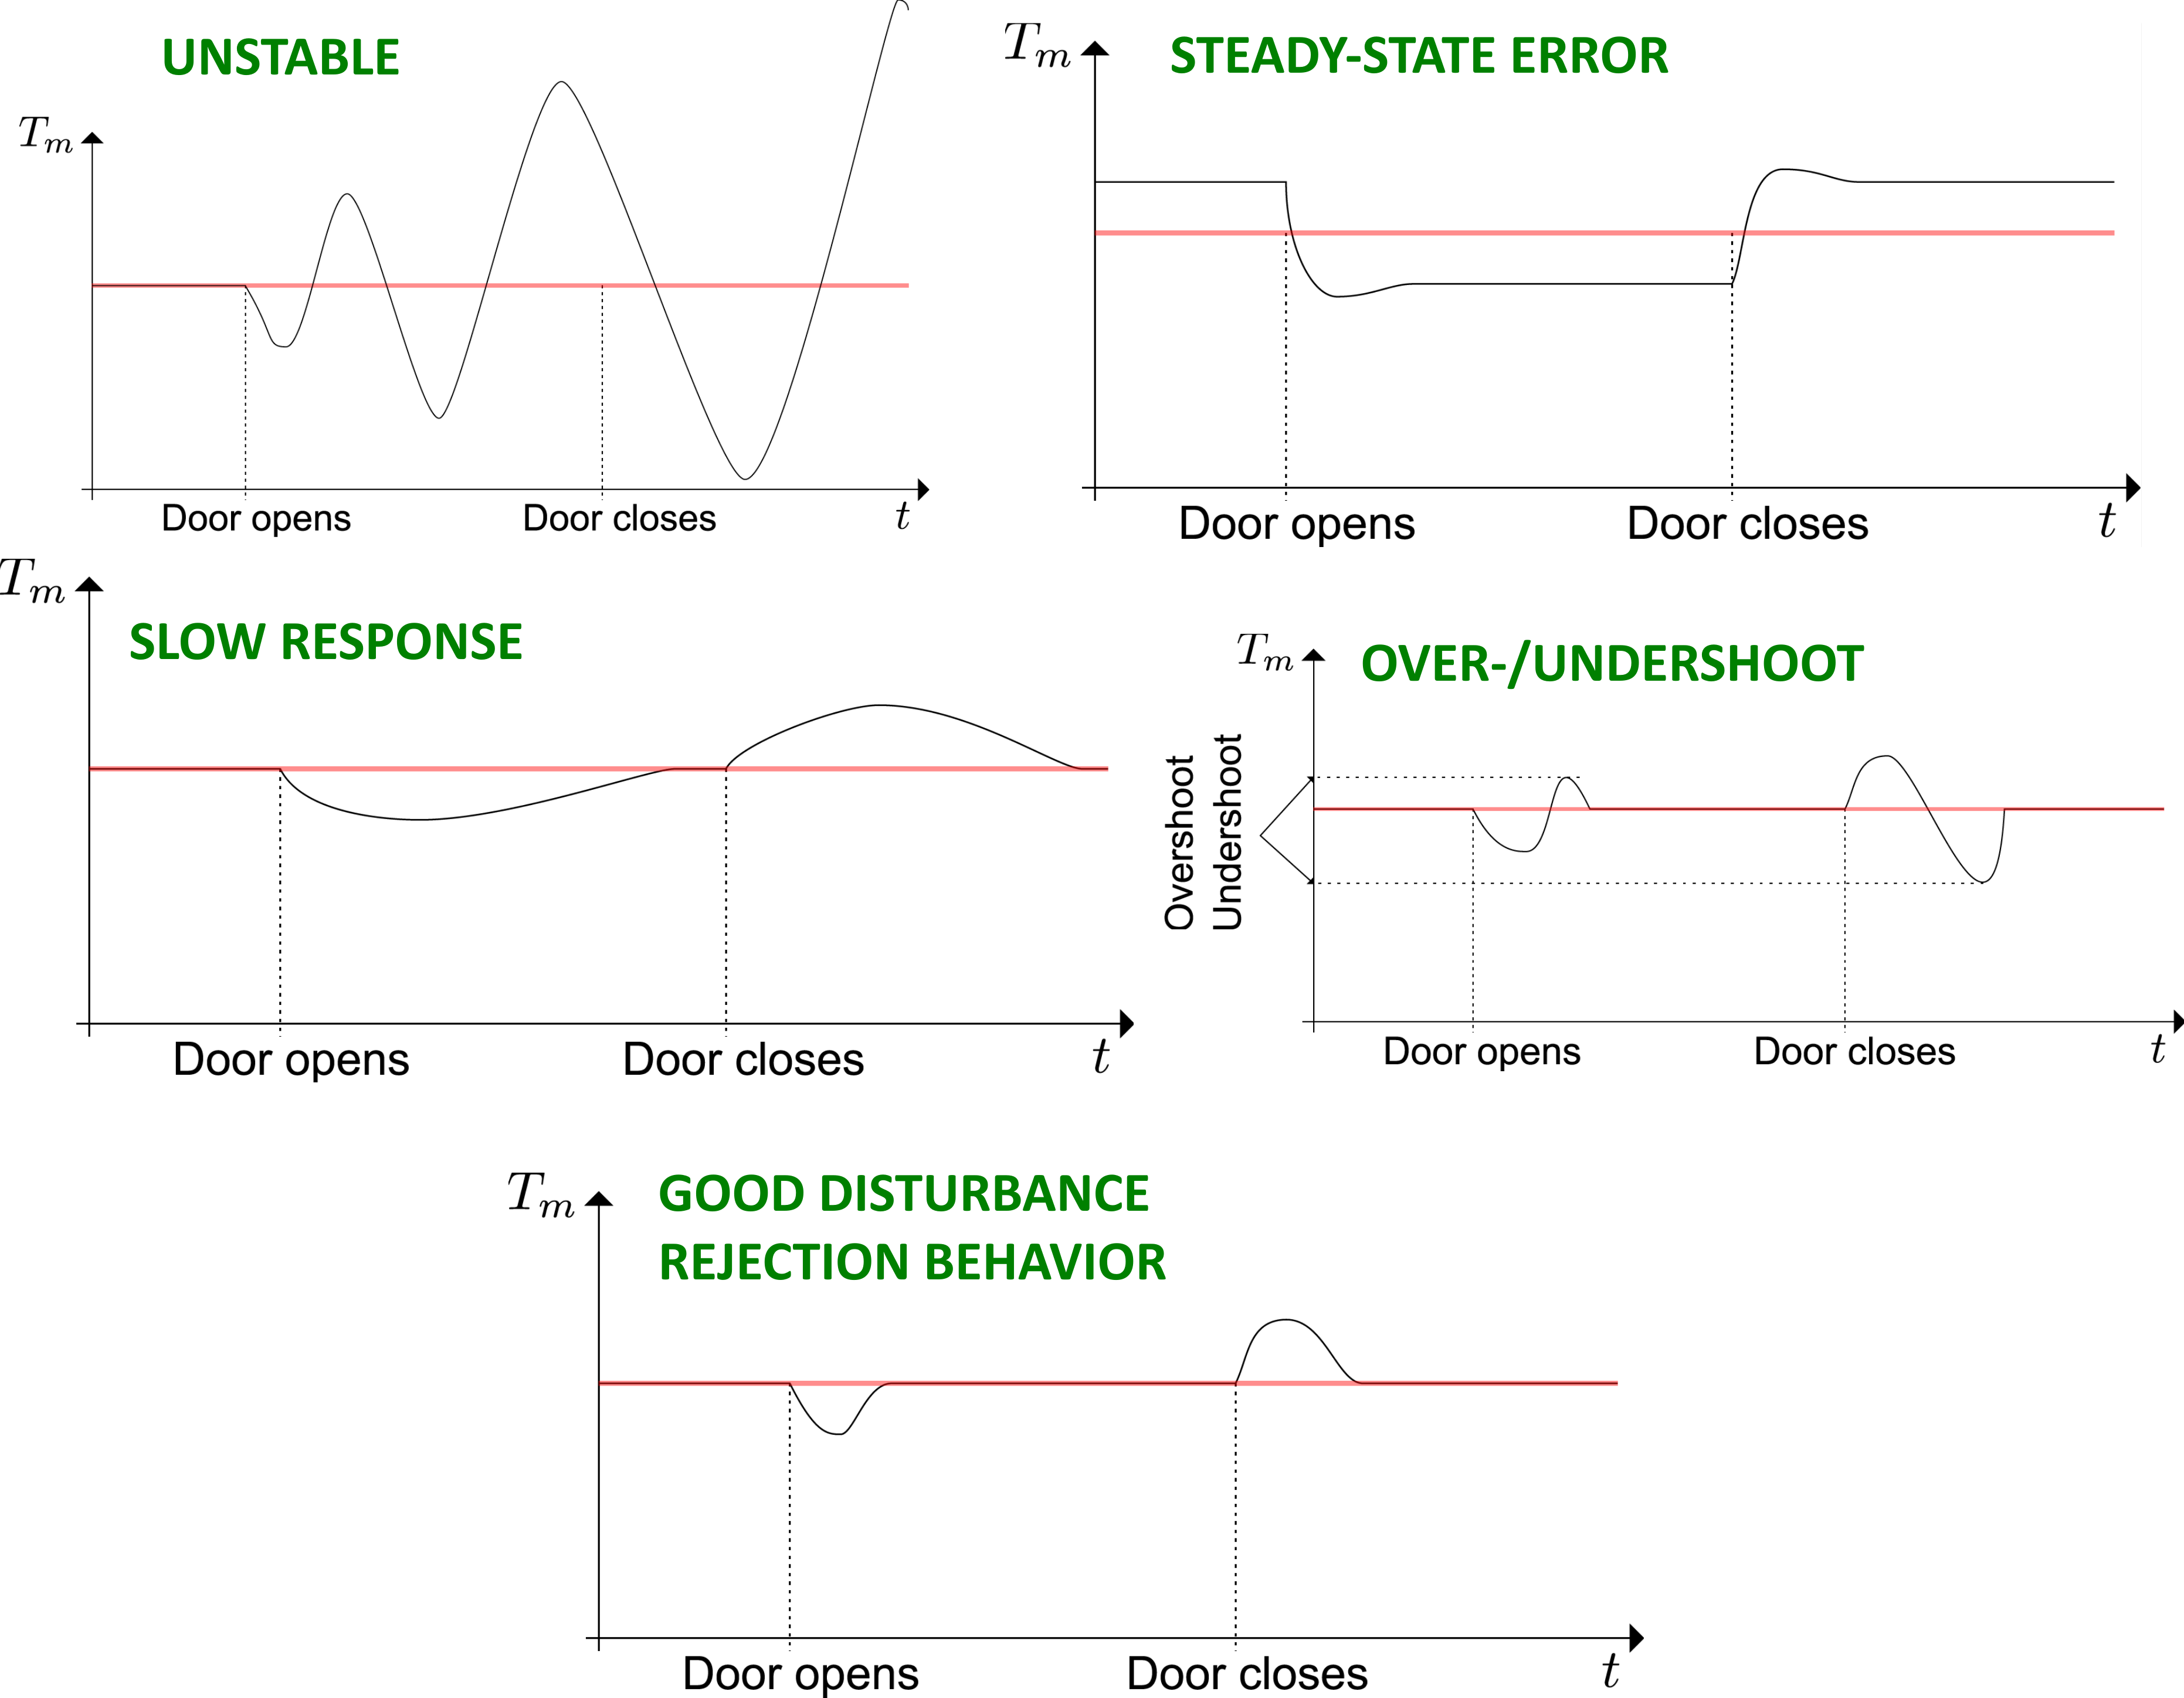
\includegraphics[\lw]{media-cheatsheet/distrej.png}

\subsection{Reference tracking}
\begin{itemize}
    \item Ability to follow the desired reference signal accurately
    \item Tracking error: difference between reference and output
\end{itemize}

\subsubsection{Characteristics}
\begin{itemize}
    \item Tracking accuracy: output follows the reference with minimal deviation
    \item Effectiveness: controller reduces tracking error under different conditions
    \item Control strategies: feedback corrects deviations; feedforward anticipates reference changes
\end{itemize}

\subsubsection{Performance metrics}
\begin{itemize}
    \item Stability: tracking remains consistent and robust
    \item Steady-state error: long-term deviation from the reference is minimized
    \item Overshoot/undershoot: excessive deviations during tracking are reduced
    \item Rise/settling time: output reaches the reference quickly and stably
\end{itemize}

\subsubsection{Graphical representation}
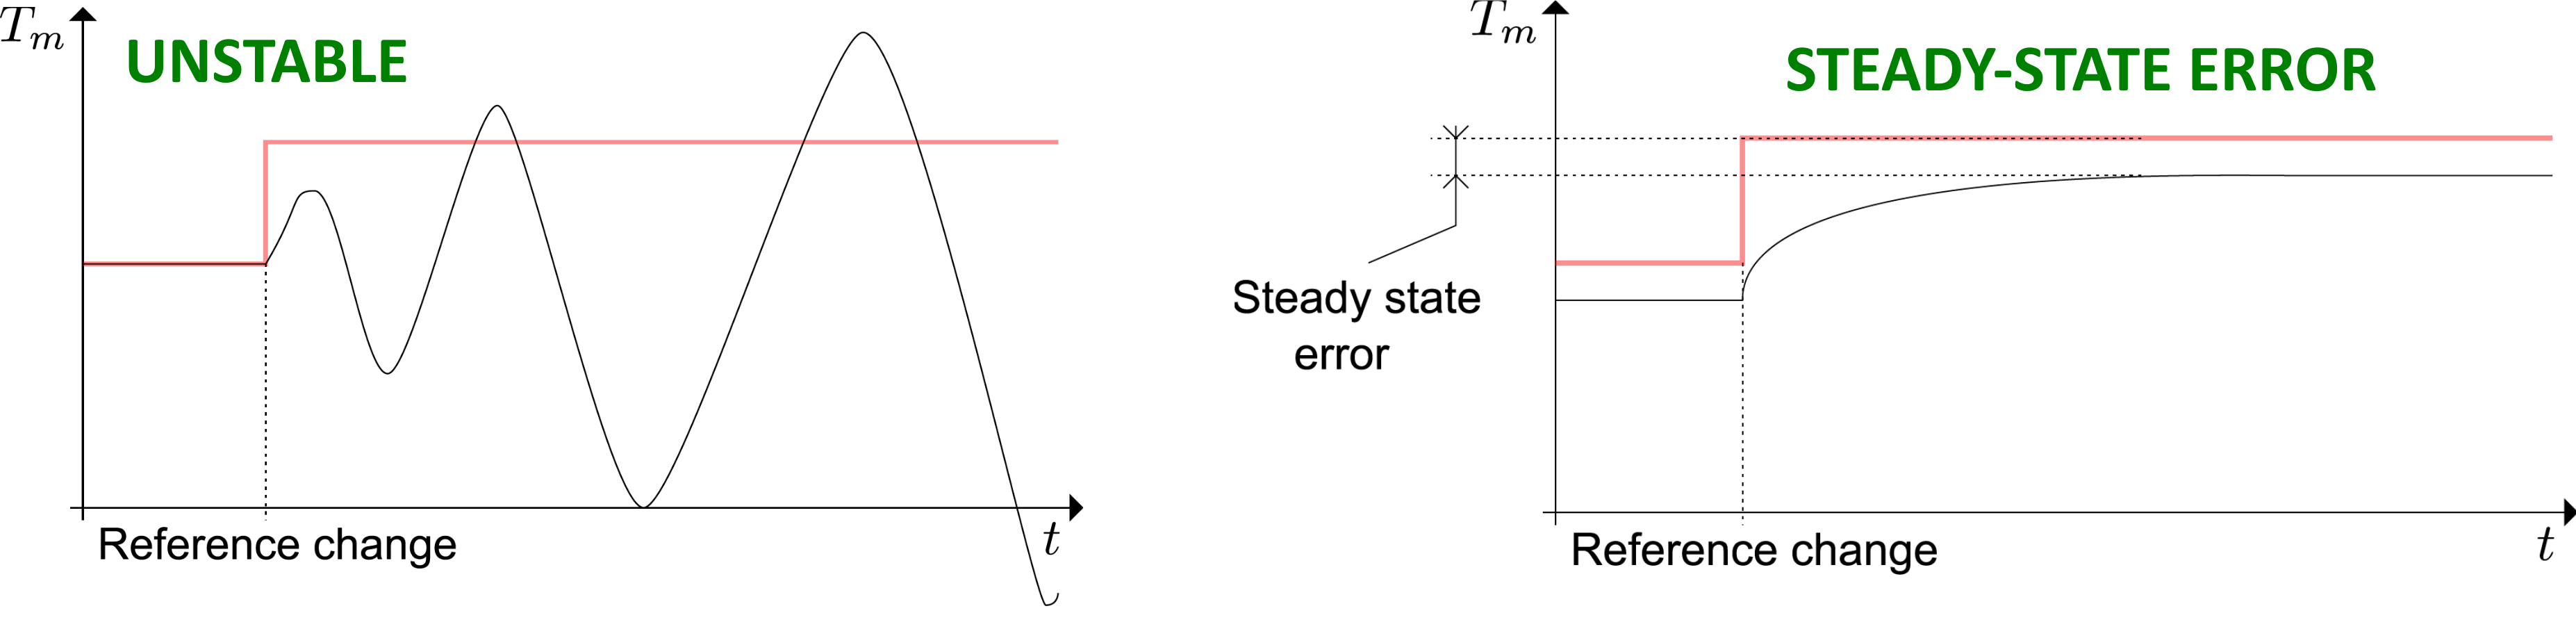
\includegraphics[\lw]{media-cheatsheet/reftra.png}

\newcolumn
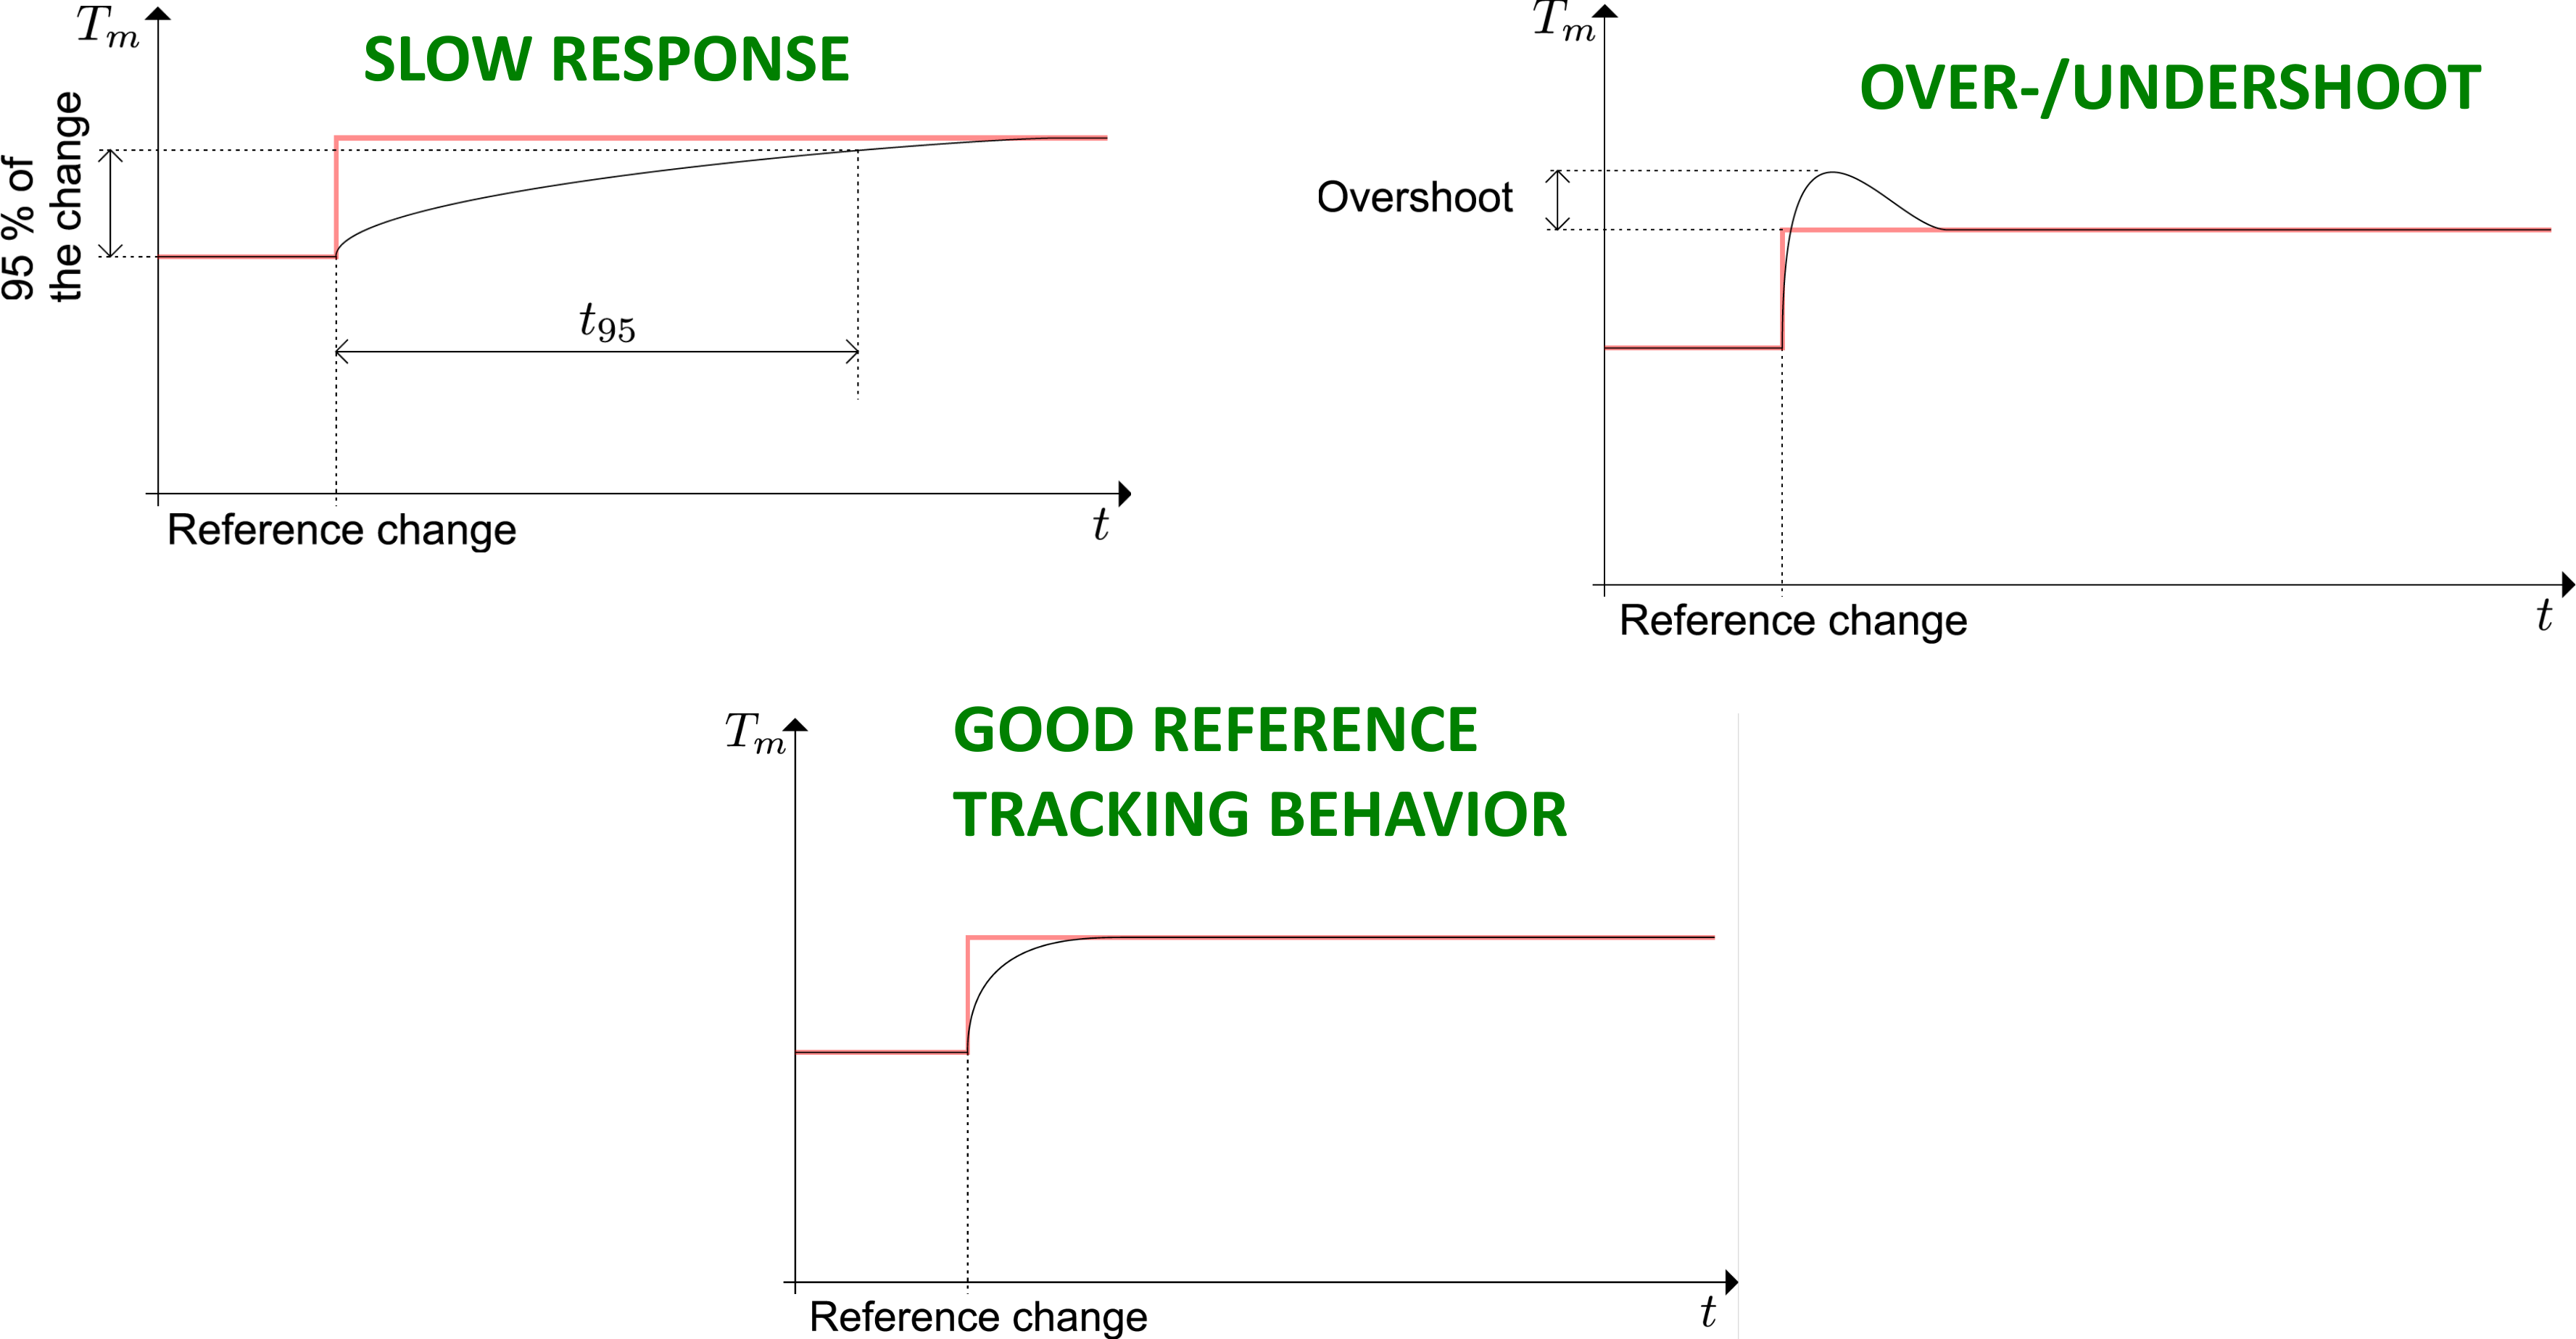
\includegraphics[\lw]{media-cheatsheet/reftra_2.png}

\section{Feedforward control}
\begin{itemize}
    \item Predictive control strategy that compensates known influences before they affect the output
    \item Improves performance by anticipating changes instead of only reacting to errors
\end{itemize}
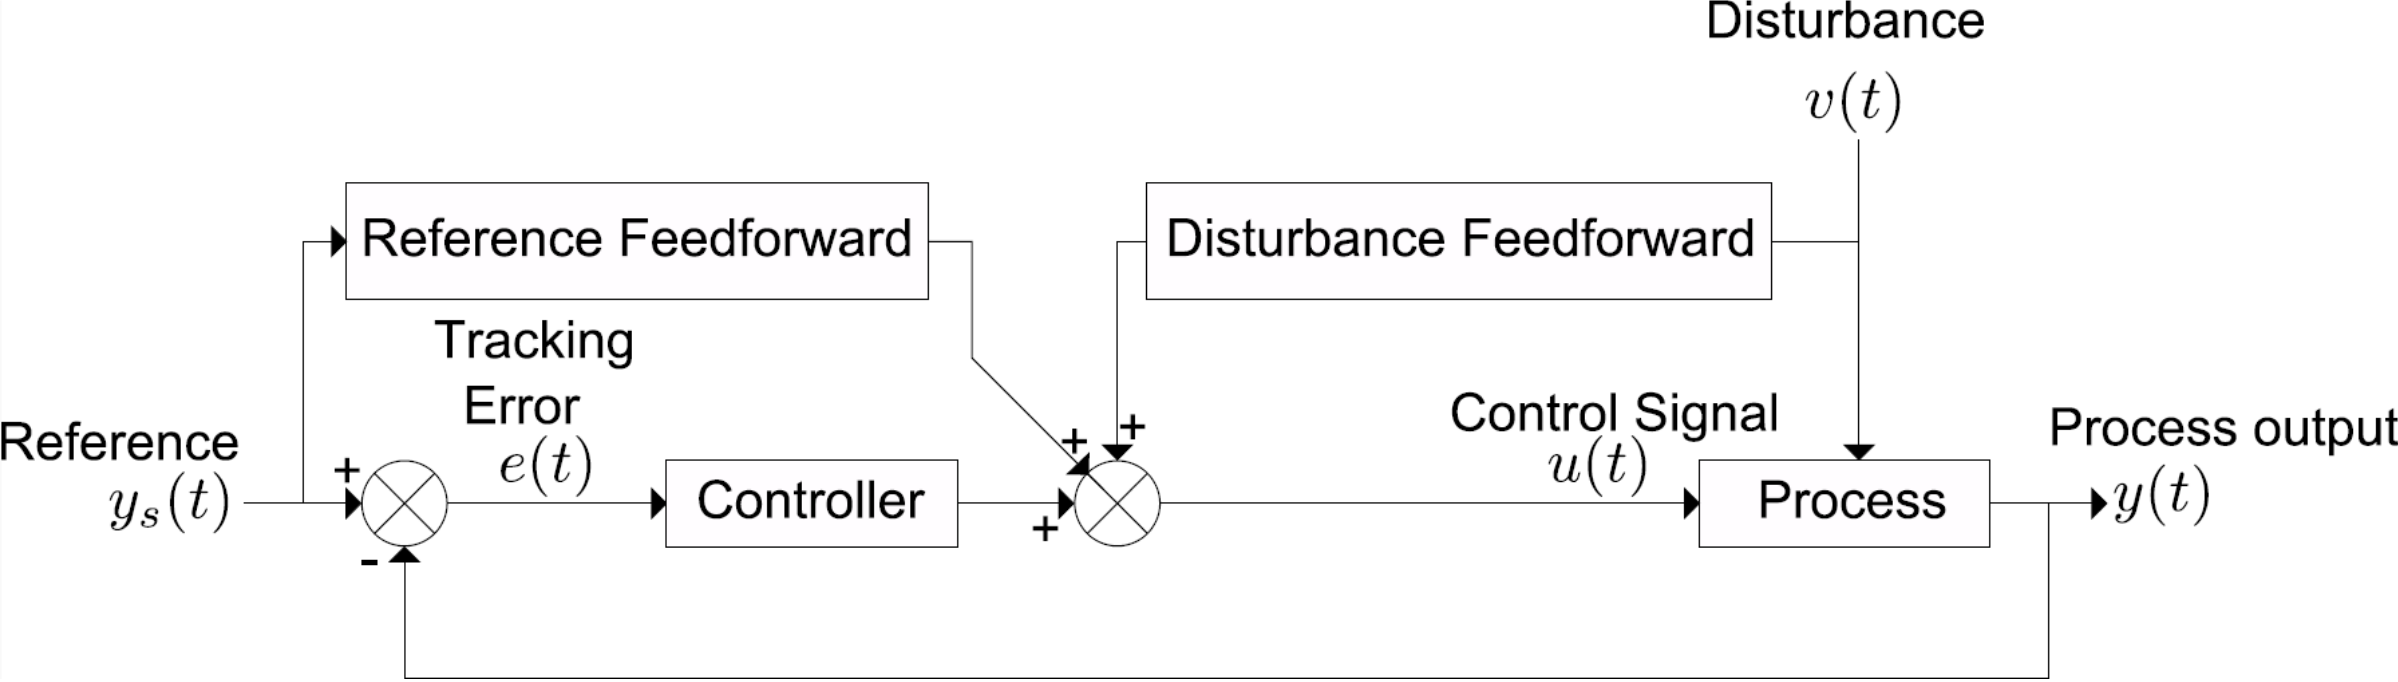
\includegraphics[\lw]{media-cheatsheet/feedforward.png}

\subsection{Reference feedforward}
\begin{itemize}
    \item Compensates reference changes before they affect the system
    \item Improves tracking by adjusting the control input in advance
\end{itemize}

\subsection{Disturbance feedforward}
\begin{itemize}
    \item Compensates measurable disturbances before they affect the output
    \item Uses a precomputed correction based on the expected disturbance effect
\end{itemize}

\part{Process model development}
\section{Damped mass-spring example}
\subsection{Differential equation}
Step 1: Set the differential equation
\[M\frac{d^2h}{dt^2}+c\frac{dh}{dt}+kh = F\]

Step 2: Isolate the term with the highest differential order
\[\frac{d^2h}{dt^2} = \frac{F}{M}-\frac{kh}{M}-\frac{c}{M}\frac{dh}{dt}\]

\subsection{ODE diagram}
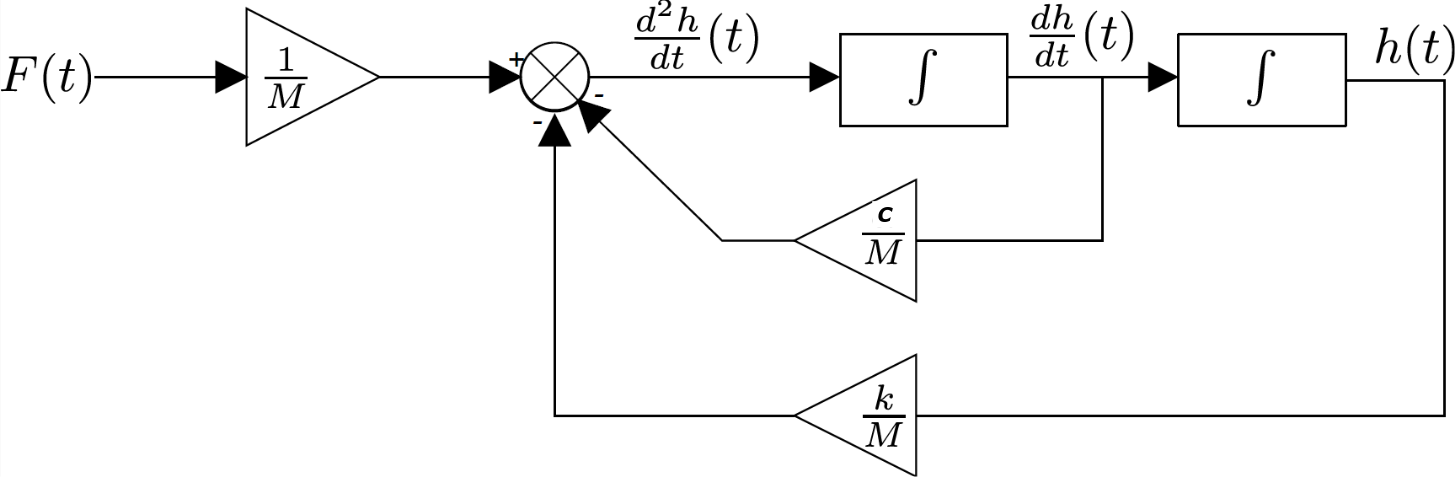
\includegraphics[\lw]{media-cheatsheet/ode-diagram.png}

\part{Signals and Systems}
\section{Homogeneity (scaling principle)}
Scaling the input by a constant also scales the output by the same constant:
\begin{itemize}
    \item If $u(t) \stackrel{h}{\to} y(t)$, then $\alpha u(t) \stackrel{h}{\to} \alpha y(t)$\\[0ex]
    \item If $y(t) = h\big(u(t)\big)$, then $h\big(\alpha u(t)\big)$, that is, $h\big(\alpha u(t)\big)=\alpha h\big(u(t)\big)$ 
\end{itemize}
\subsection{Graphical visualization}
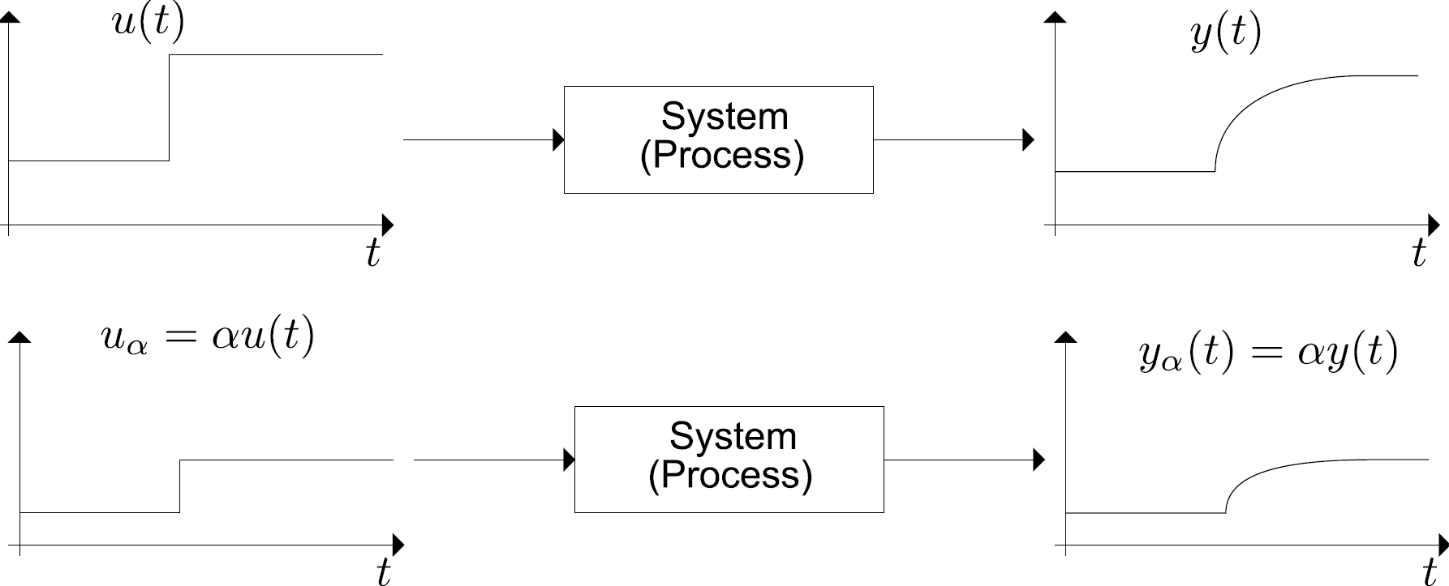
\includegraphics[\lw]{media-cheatsheet/homogeneity.png}

\subsection{Homogeneity proof examples}
\subsubsection{Homogeneous system}
\begin{gather*}
    u(t) \stackrel{h}{\to} y(t) = 4u(t)\\
    h(\alpha u(t)) = 4(\alpha u(t)) = \alpha(4u(t)) = \alpha h(u(t))\\
    \alpha u(t) \stackrel{h}{\to} \alpha y(t) \tag*{$\Box$}
\end{gather*}

\subsubsection{Non-homogeneous system}
\begin{gather*}
    u(t) \stackrel{h}{\to} y(t) = u^3(t)\\
    h(\alpha u(t)) = (\alpha u(t))^3 = \alpha^3 y(t) \neq \alpha y(t)\\
    h(\alpha u(t)) \neq \alpha h(u(t)) \tag*{$\Box$}
\end{gather*}
\newcolumn

\section{Additivity (superposition principle)}
The output of summed inputs equals the sum of the individual outputs:
\begin{itemize}
    \item If $u_1(t) \to y_1(t)$ and $u_2(t) \to y_2(t)$, then
        \[u_1(t) + u_2(t) \to y_1(t) + y_2(t)\]
    \item If $y_1(t) = h(u_1(t))$ and $y_2(t)=h(u_2(t))$, then
        \[h(u_1(t) + u_2(t)) = y_1(t) + y_2(t)\]
        \hspace*{.2cm} That is
        \[h(u_1(t) + u_2(t)) = h(u_1(t))+h(u_2(t))\]
\end{itemize}
\subsection{Graphical visualization}
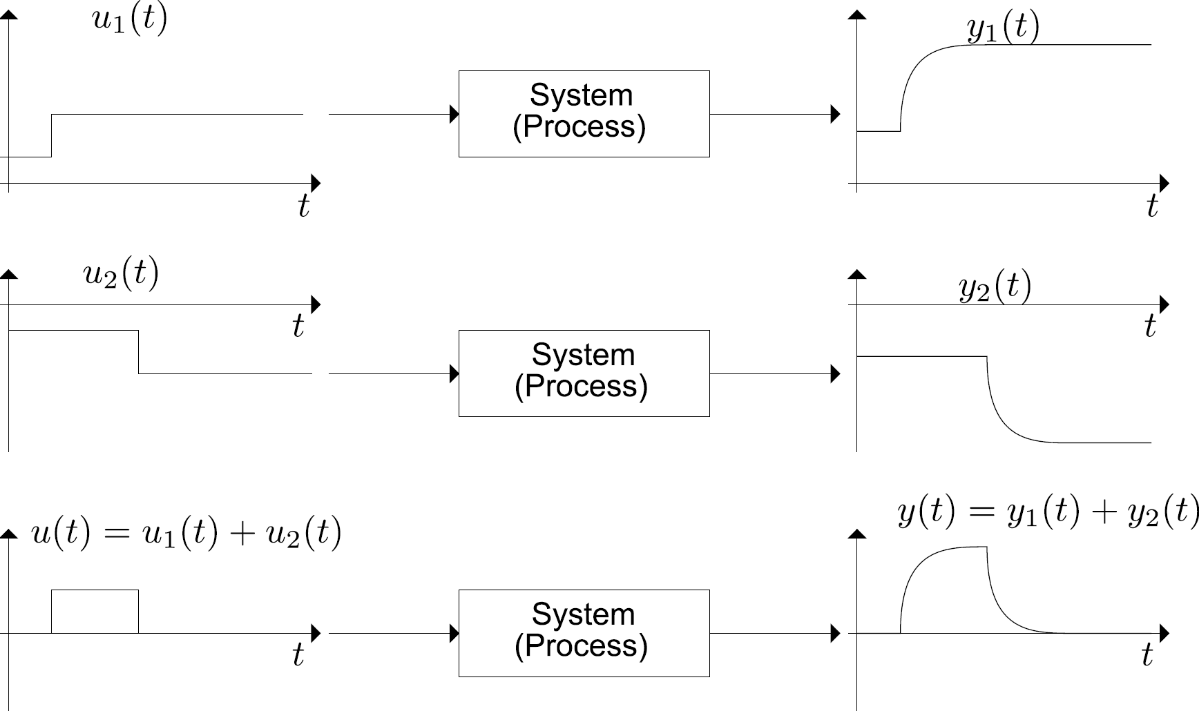
\includegraphics[\lw]{media-cheatsheet/additivity.png}

\subsection{Additivity proof examples}
\subsubsection{Additive system}
\begin{gather*}
    u_1(t) \stackrel{h}{\to} y_1(t) = 2u_1(t)\\
    u_2(t) \stackrel{h}{\to} y_2(t) = 2u_2(t)\\
    h\big(u_1(t) + u_2(t)\big) = 2\big(u_1(t) + u_2(t)\big)\\
    = 2u_1(t) + 2u_2(t) = y_1(t) + y_2(t)\\
    u_1(t) + u_2(t) \stackrel{h}{\to} y_1(t) + y_2(t) \tag*{$\Box$}
\end{gather*}

\subsubsection{Non-additive system}
\begin{gather*}
    u(t) \stackrel{h}{\to} y(t) = \sin(u(t))\\
    h(u_+(t) + u_2(t)) = \sin(u_1(t)+u_2(t)) \neq \sin(u_1(t)) + \sin(u_2(t)) \tag*{$\Box$}
\end{gather*}

\section{Linear system}
A system is linear if it satisfies both the homogeneity (scaling) and additivity principles.

\newcolumn
\section{Time-invariant system}
System behavior does not change over time. A time-shifted input produces the same time-shifted output:
\begin{itemize}
    \item If $u(t) \to y(t)$, then
        \[u(t-t_0) \to y(t-t_0)\]
    \item If $y(t) = h(u(t))$, then
        \[h(z(t-t_0)) = y(t-t_0)\]
\end{itemize}

\subsection{Time-invariance proof example}
\subsubsection{Time-invariant system}
\begin{gather*}
    u(t) \stackrel{h}{\to} y(t) = u(t) + 7\\
    h\big(u(t-t_0)\big) = u(t-t_0) + 7 = y(t-t_0)\\
    u(t-t_0) \stackrel{h}{\to} y(t-t_0) \tag*{$\Box$}
\end{gather*}

\subsubsection{Time-variant system}
\begin{gather*}
    u(t) \stackrel{h}{\to} y(t) = u(t) + t\\
    h\big(u(t-t_0)\big) = u(t-t_0) + t\\
    y(t-t_0) = u(t-t_0) + (t-t_0)\\
    h\big(u(t-t_0)\big) \neq y(t-t_0) \tag*{$\Box$}
\end{gather*}

\section{Digitalization}
\begin{center}
    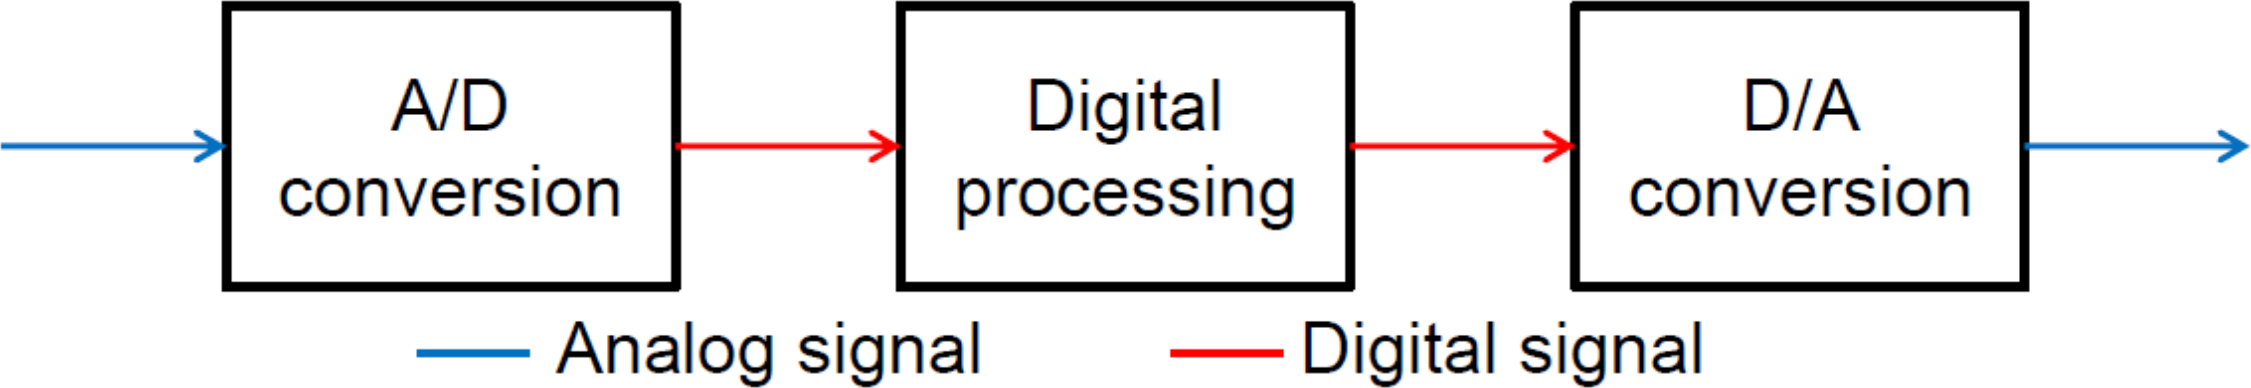
\includegraphics[\lw=0.8]{media-cheatsheet/ADDA.png}
\end{center}
\subsection{Time discretization}
\begin{itemize}
    \item Sampling: continuous signal measured at fixed time intervals
    \item Sampling rate: number of samples per second [Hz or kHz]
\end{itemize}

\subsection{Amplitude discretization}
\begin{itemize}
    \item Quantization: signal values are rounded to discrete levels
    \item Quantization type: uniform uses equal steps; non-uniform uses variable steps
    \item Quantization step: coarse steps give lower precision; fine steps give higher precision
\end{itemize}

\subsection{Basic input signals}
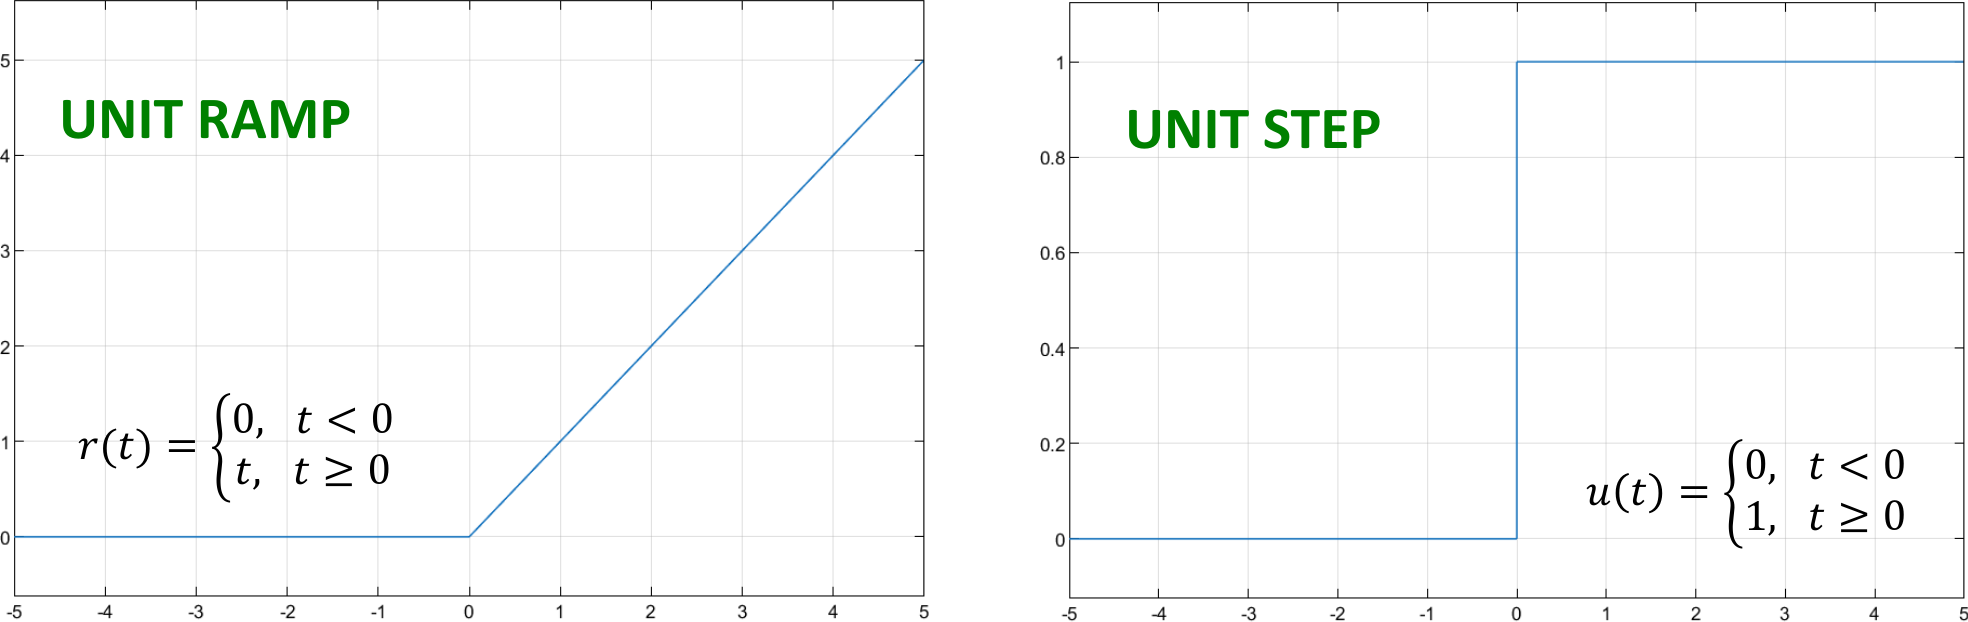
\includegraphics[\lw]{media-cheatsheet/inputsignal.png}

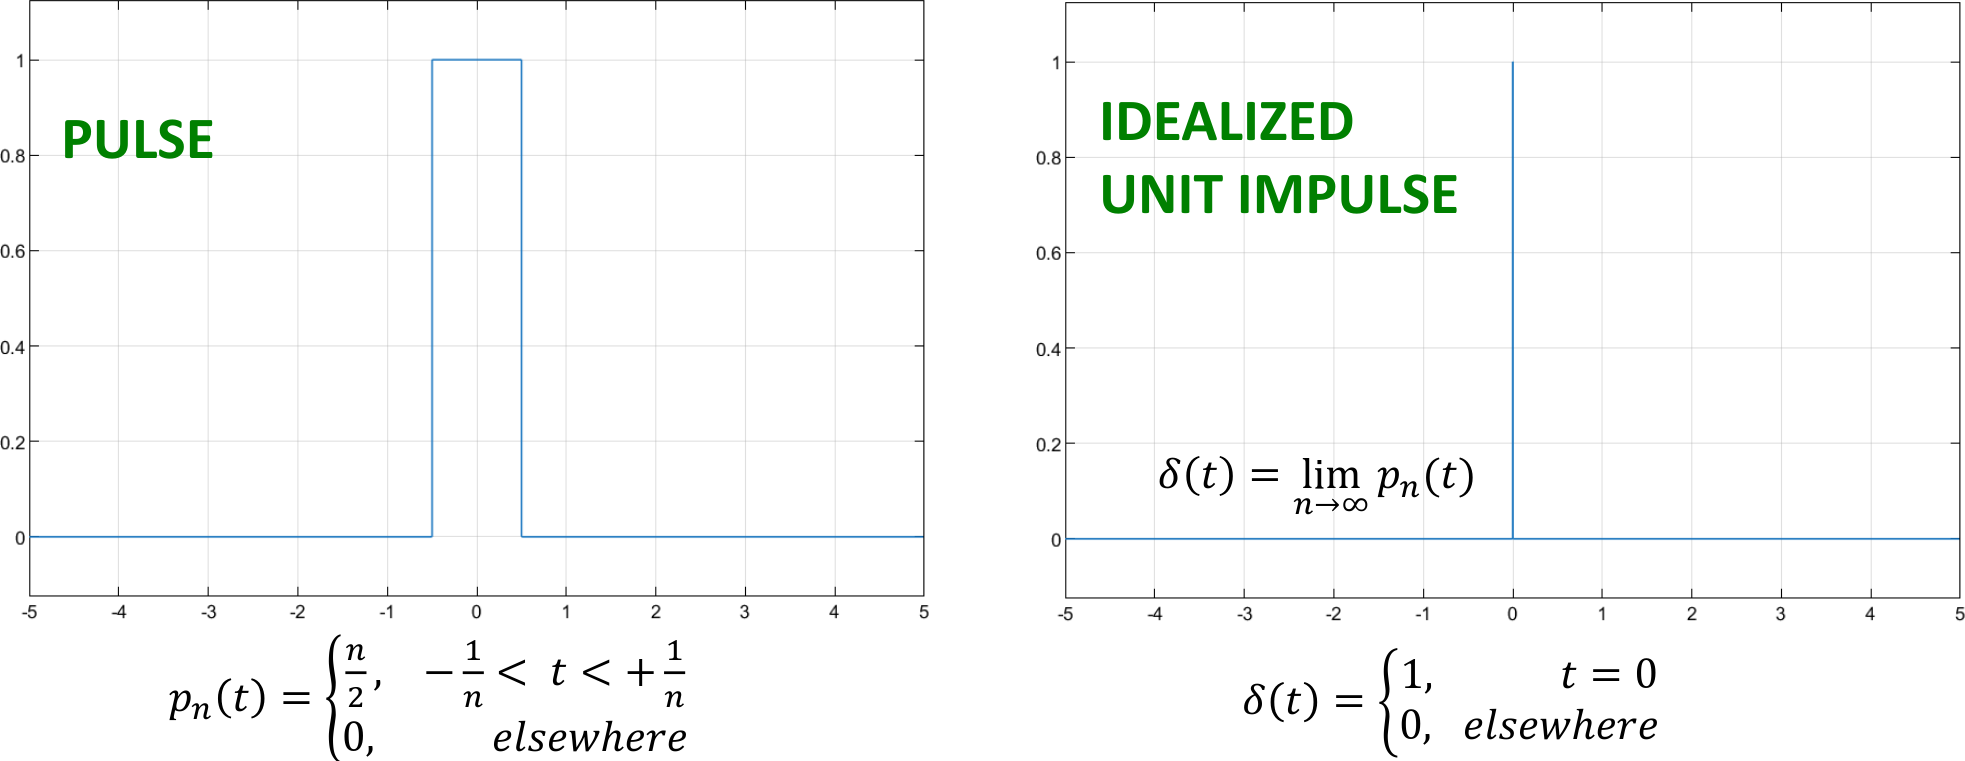
\includegraphics[\lw]{media-cheatsheet/inputsignal2.png}

\part{Linearization}
\section{Steps for linearizing a function}
\begin{enumerate}[label=Step \arabic*.]
    \item Determine the nonlinear differential equation:
        \[M\ddot{h}+c\dot{h}=Mg-kh^3\]
    \item Define $f(\ddot{h},\dot{h},h)=0$:
        \[M\ddot{h}+c\dot{h}+kh^3-Mg=0\]
    \item Define the slopes $\Delta$:
        \[\Delta \ddot{h} = \ddot{h} - \overline{\ddot{h}}\]
    \item Calculate the partial derivatives of $f$ at the steady state for all the variables:
        \[\frac{\partial f}{\partial \ddot{h}} = M\Delta\ddot{h}\]
    \item Establish a linear equation using the slopes solving for the highest differential order:
        \[\Delta\ddot{h} = -\frac{c}{M}\Delta\dot{h} - \frac{3k(\overline{h})^2}{M}\Delta h\]
\end{enumerate}

\subsection{ODE diagram}
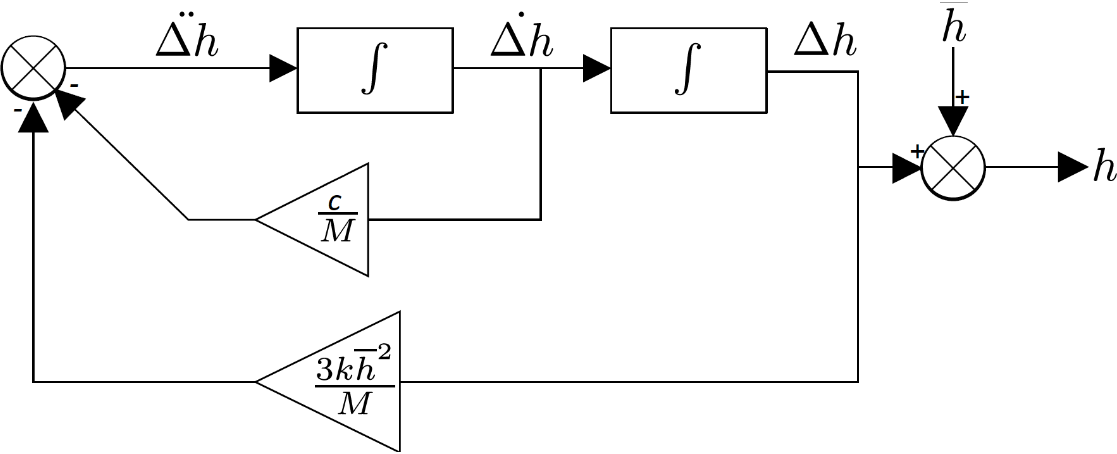
\includegraphics[\lw]{media-cheatsheet/linearization.png}

\part{Controllers}
\section{Analog controller}
\begin{itemize}
    \item Processes continuous signals using analog components, e.g. resistors, capacitors, and operational amplifiers
    \item Control signal: continuous voltage or current
    \item Main feature: fast real-time response with simple control logic
\end{itemize}

\newcolumn
\section{Digital controller}
\begin{itemize}
    \item Uses A/D and D/A converters $\to$\ discretization and delays
    \item Slightly reduced dynamic performance due to discretization
    \item Flexible, precise, scalable, and easy to maintain
    \item Compact and cost-effective hardware
    \item Supports multitasking, noise filtering, and advanced algorithms
\end{itemize}

\subsection{Implementation platforms}
\begin{itemize}
    \item IPCs: complex real-time industrial control
    \item MCUs: simple low-cost embedded control
    \item PLCs: robust automation in harsh environments
    \item DSPs: fast real-time signal calculations
    \item FPGAs: ultra-fast parallel control
    \item SBCs: prototyping and low-cost control
    \item Cloud: remote monitoring, control, and data analysis
\end{itemize}

\subsection{Architecture and communication}
\begin{itemize}
    \item Centralized control: one unit handles processing, conversion, inputs, and outputs; simple but less scalable
    \item Fieldbus communication: distributed devices communicate via industrial networks; scalable and modular
    \item Examples: ProfiNET, CAN/CANopen, EtherCAT
\end{itemize}

\subsection{2-point controller}
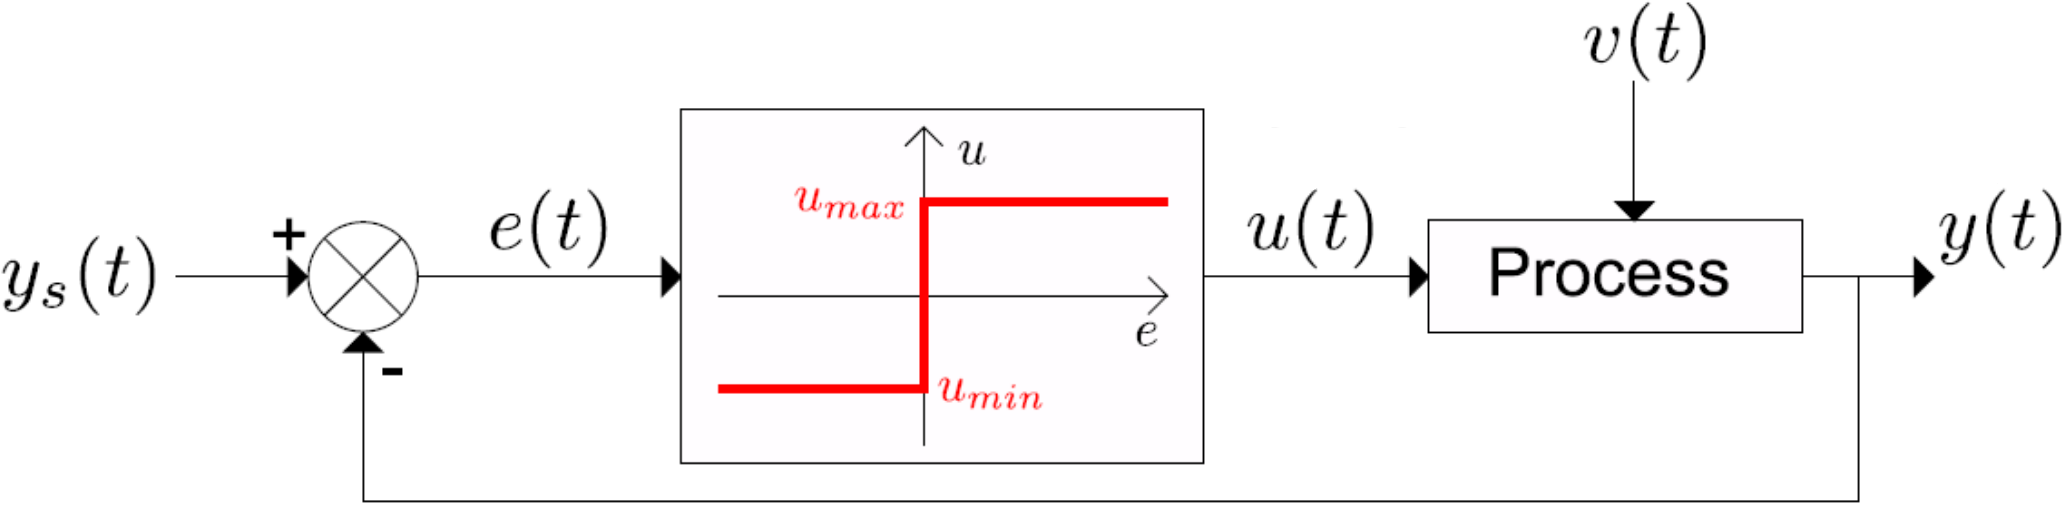
\includegraphics[\lw]{media-cheatsheet/2step.png}
\[\begin{cases}
    u = u_{max} &\text{if  } e > 0\\
    u = u_{min} &\text{if  } e < 0
\end{cases}\]

\subsubsection{2-point controller with hysteresis}
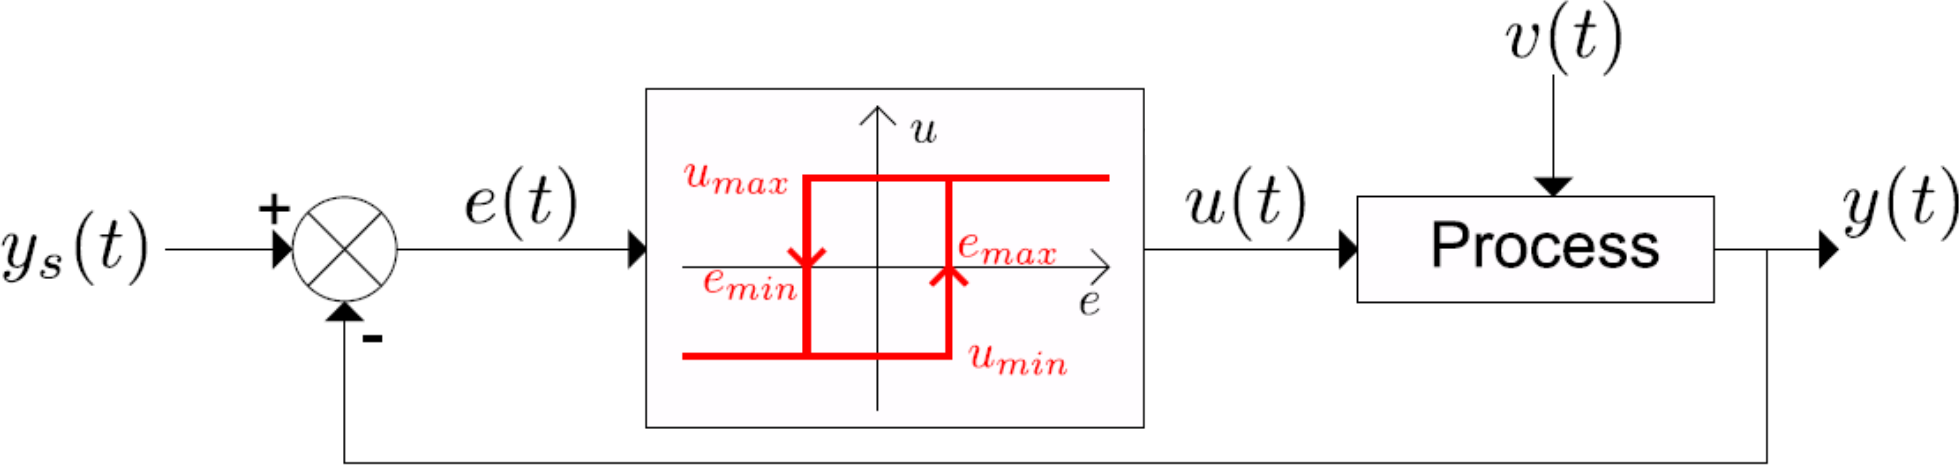
\includegraphics[\lw]{media-cheatsheet/2step-hyst.png}
\[\begin{cases}
    u = u_{max} &\text{if  } e > e_{max}\\
    u = u_{max} &\text{if  } e_{min} < e < e_{max} \text{ and } \dot{e} < 0\\
    u = u_{min} &\text{if  } e_{min} < e < e_{max} \text{ and } \dot{e} > 0\\
    u = u_{min} &\text{if  } e < e_{min}
\end{cases}\]

\subsection{3-point controller}
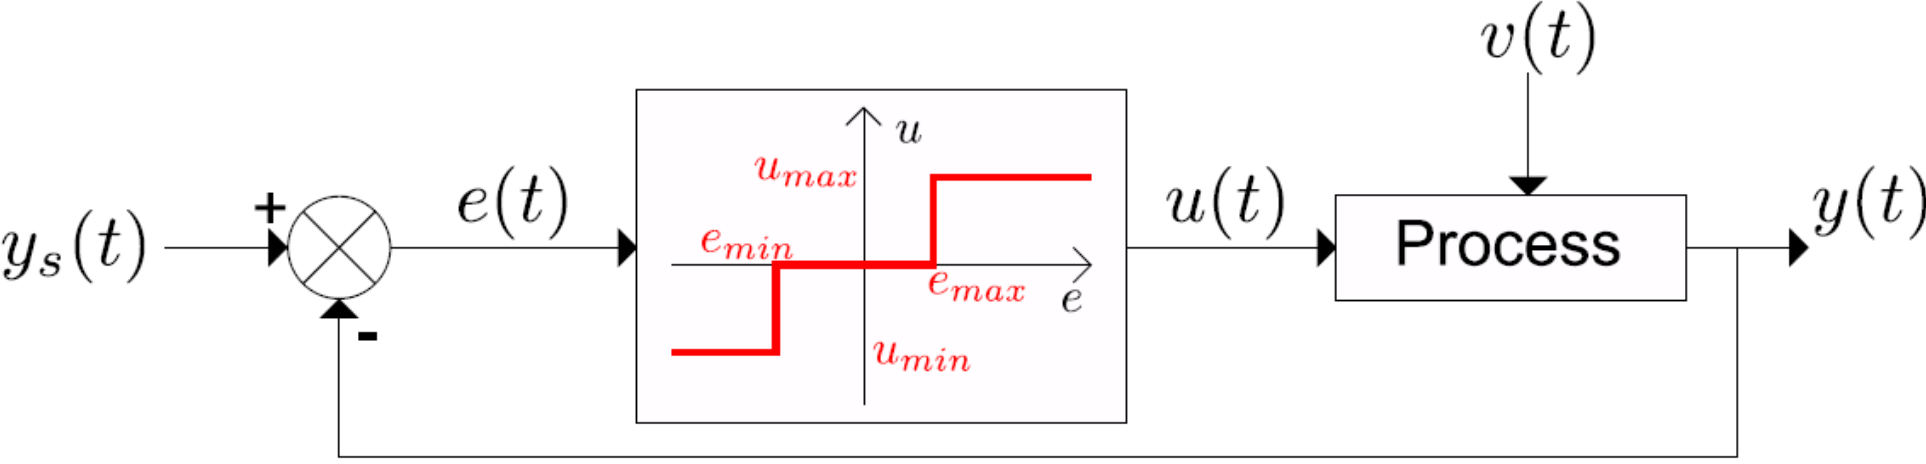
\includegraphics[\lw]{media-cheatsheet/3step.png}
\[\begin{cases}
    u = u_{max} &\text{if  } e > e_{max}\\
    u = 0       &\text{if  } e_{min} < e < e_{max}\\
    u = u_{min} &\text{if  } e < e_{min}
\end{cases}\]

\subsection{Proportional-Integral-Derivative (PID) controller}
\subsubsection{Mathematical parametrization}
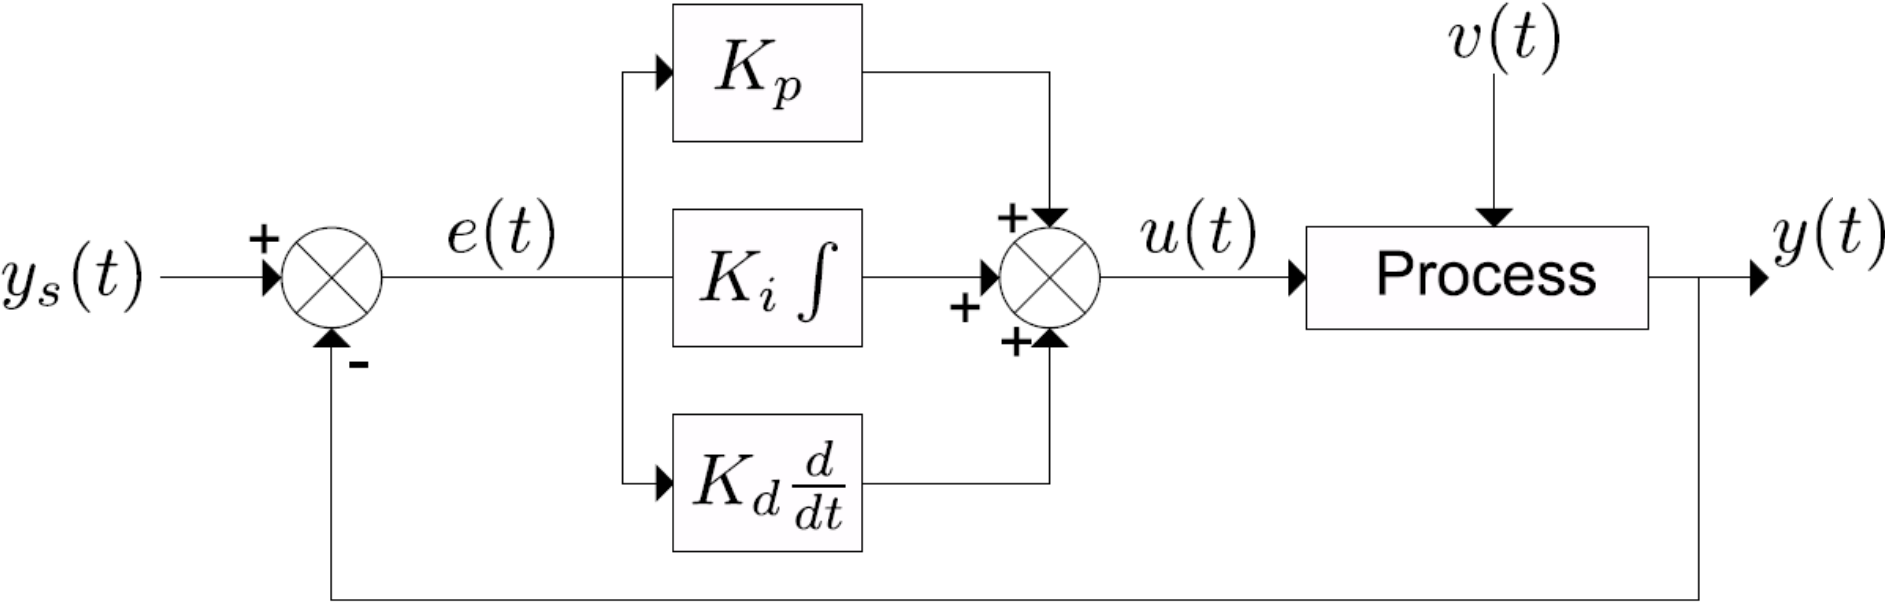
\includegraphics[\lw]{media-cheatsheet/PID.png}
\[\dm u(t) = K_p(e(t)) + K_i\integral[0][t][e(\tau)][\tau] + K_d\frac{de(t)}{dt}\]

\subsubsection{Technical usual parametrization}
\begin{center}
    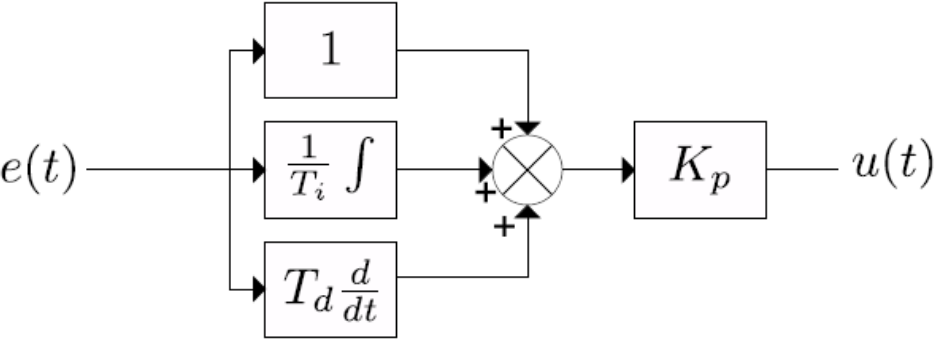
\includegraphics[\lw=.8]{media-cheatsheet/PID2.png}
\end{center}
\[\dm u(t) = K_p\left(e(t) + \frac{1}{T}\integral[0][t][e(\tau)][\tau]+T_d\frac{de(t)}{dt}\right)\]
\begin{center}
    \begin{tabular}{ccc}
        Controller gain & Integral time & Derivative time\\
        $K_p$ & $\dm T_i = \frac{K_p}{K_i}$ & $\dm T_d = \frac{K_d}{K_p}$
    \end{tabular}
\end{center}

\subsection{PID principle}
\pph{Proportional term (P)}
\vspace*{-.6cm}
\begin{itemize}
    \item Immediate correction proportional to current error
    \item Reduces rise time
    \item Cannot remove steady-state error alone
    \item Too high $\to$\ oscillation/overshoot
\end{itemize}

\newcolumn
\pph{Integral term (I)}
\vspace*{-.6cm}
\begin{itemize}
    \item Eliminates steady-state error
    \item Slow reaction
    \item Large integral action $\to$\ overshoot (integral wind-up)
\end{itemize}
\vspace*{-.4cm}

\pph{Derivative term (D)}
\vspace*{-.6cm}
\begin{itemize}
    \item Predictive action: reacts to error rate of change
    \item Reduces overshoot and oscillations
    \item Sensitive to noise
\end{itemize}

\begin{minipage}{0.48\linewidth}
    \pph{PI controller}
    \vspace*{-.4cm}
    \begin{itemize}
        \item Faster than pure I
        \item Deletes steady-state error
        \item Mild overshoot
    \end{itemize}
\end{minipage}%
\begin{minipage}{0.48\linewidth}
    \pph{PD controller}
    \vspace*{-.4cm}
    \begin{itemize}
        \item Fast response
        \item Low overshoot
        \item Still has steady-state error
    \end{itemize}
\end{minipage}
\vspace*{-.4cm}

\pph{PDI controller}
\vspace*{-.6cm}
\begin{itemize}
    \item Fast rise time
    \item No steady-state error
    \item Limited overshoot
    \item Best compromise between accuracy + stability
\end{itemize}

\subsubsection{Graphical representation}
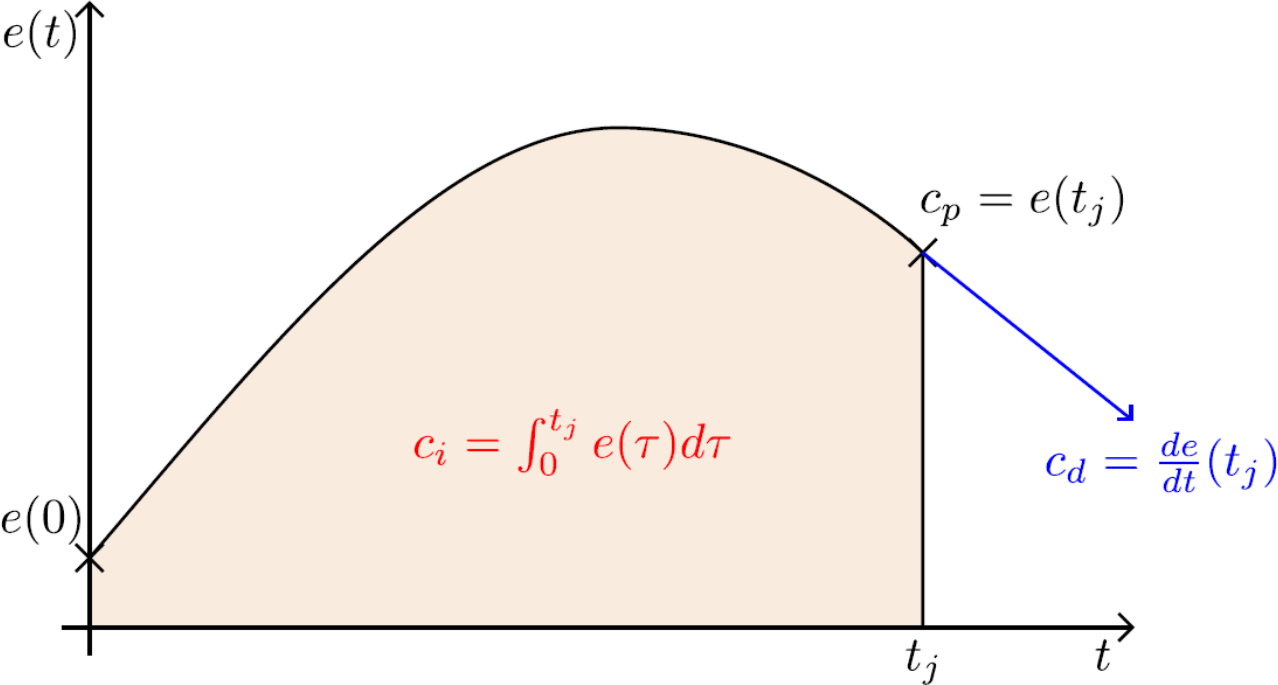
\includegraphics[\lw]{media-cheatsheet/PID-graph.png}

\part{Laplace transform}
\section{Laplace transform}
The Laplace transform is defined for $t \geq 0$ as
\figbox{$\dm F(s) = \mathcal{L}\{f(t)\} = \integral[0][\infty][f(t)\cdot e^{-st}][t]$}
\begin{center}
    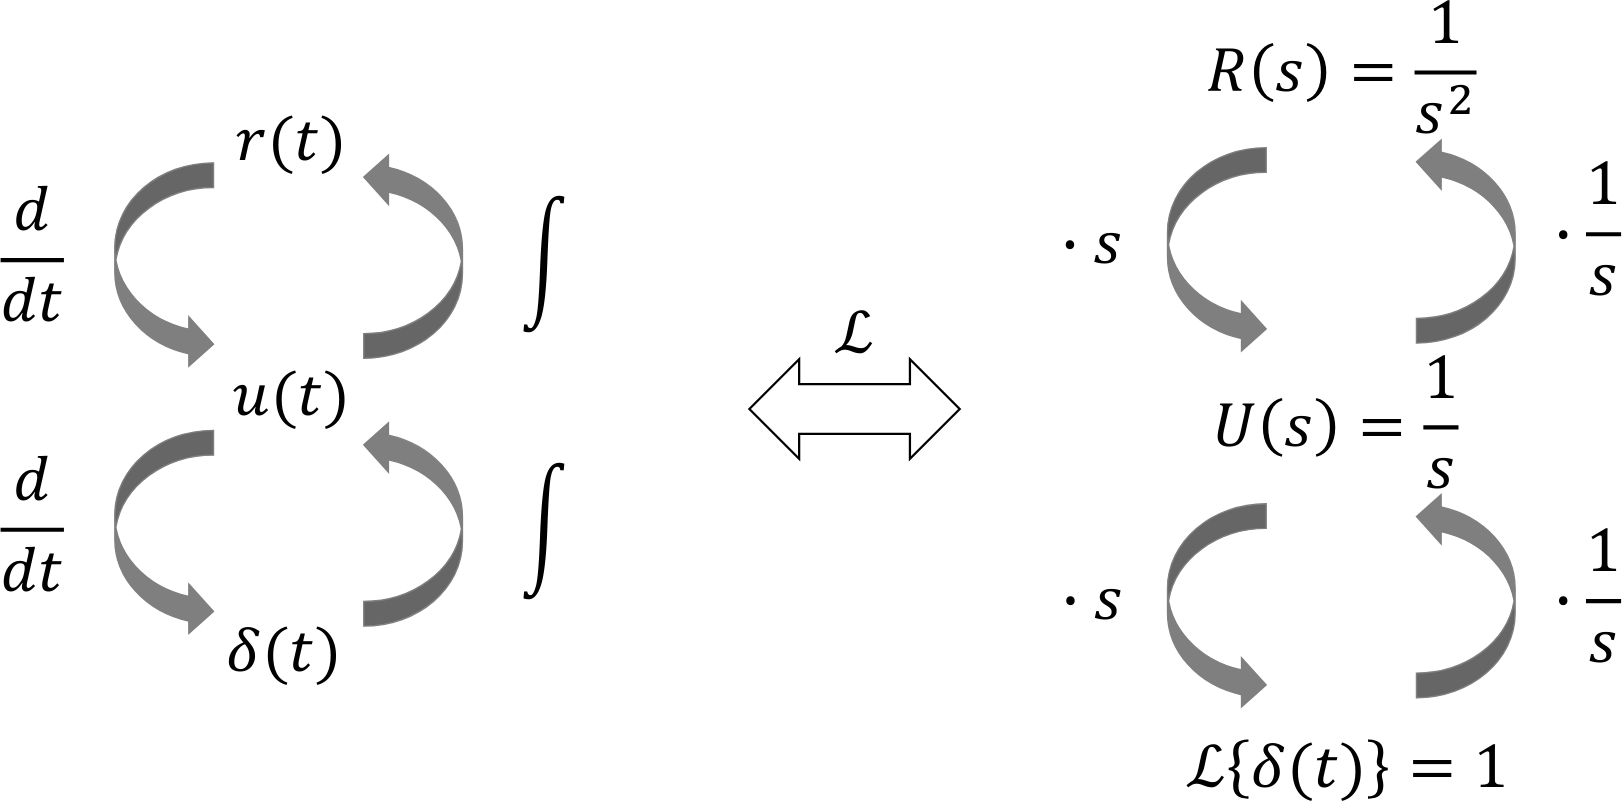
\includegraphics[\lw=.72]{media-cheatsheet/Laplace.png}
\end{center}

\subsection{Laplace transform of some functions}
\begin{center}
    \footnotesize
    \setcellgapes{2pt}
    \makegapedcells
    \begin{tabularx}{\linewidth}{|l|X|X|}
        \hline & $\bm{f(t),\ t \geq 0}$ & $\bm{F(s) = \mathcal{L}\{f(t)\}}$\\
        \hline Constant & $1\quad ;\quad a$ & $\dfrac{1}{s}\quad ;\quad \dfrac{a}{s}$\\
        \hline Step function & $t\quad ;\quad at$ & $\dfrac{1}{s^2}\quad ;\quad \dfrac{a}{s^2}$\\
        \hline Derivative & $\dfrac{df(t)}{dt}$ & $sF(s)-f(0)$\\
        \hline Integral & $\displaystyle\int_0^t f(\tau)\,d\tau$ & $\dfrac{1}{s} F(s)$\\
        \hline Initial value & $\displaystyle\lim_{t\to 0} f(t)$ & $\displaystyle\lim_{s\to\infty} sF(s)$\\
        \hline Steady-state value & $\displaystyle\lim_{t\to\infty} f(t)$ & $\displaystyle\lim_{s\to 0} sF(s)$\\
        \hline Delayed input & $f(t-t_0)$ & $\exp(-s\cdot t_0) F(s)$\\
        \hline Exponential & $\exp(-at)$ & $\dfrac{1}{s+a}$\\
        \hline 
    \end{tabularx}
    \nomakegapedcells
\end{center}

\subsection{Benefits of analysis in the s-domain}
\begin{itemize}
    \item Converts differential equations into algebraic equations
    \item Defines direct input-output relation using transfer functions
    \item Enables frequency response analysis
    \item Simplifies stability and system behavior analysis
    \item Supports structured open-loop and closed-loop analysis
    \item Makes transfer functions easier to manipulate
\end{itemize}

\part{Transfer functions}
\begin{gather*}
    sY(s) + C(s)Y(s) = G(s)u(s) \Longrightarrow Y(s)\left[s + C(s)\right] = G(s)u(s)\\[0ex]
    H_{Y,U}(s) = \dfrac{Y(s)}{U(s)} = \dfrac{C(s)}{s+G(s)} = \dfrac{K_Y}{1+\tau_Y \cdot s}
\end{gather*}

where $K_Y$ is the gain and $\tau_Y$ is the time constant.

\section{Transfer function of the PID controller}
ODE of the PID controller:
\[u(t) = K_p\left(e(t) + \frac{1}{T_i}\integral[0][t][e(\tau)][\tau] + T_d\dot{e}(t)\right)\]

Transfer function:
\begin{gather*}
    U(s) = K_p\left(E(s) + \frac{1}{T_i}\frac{E(s)}{s}+T_dsE(s)\right)\\[1ex]
    U(s) = E(s)\left(K_p\frac{T_iT_ds^2+T_is+1}{T_is}\right)\\[1ex]
    \boxed{C(s) = \frac{U(s)}{E(s)} = \left(K_p\frac{T_iT_ds^2+T_is+1}{T_is}\right)}
\end{gather*}

\newcolumn
\section{Block diagram manipulation}
\subsection{Serial connection}
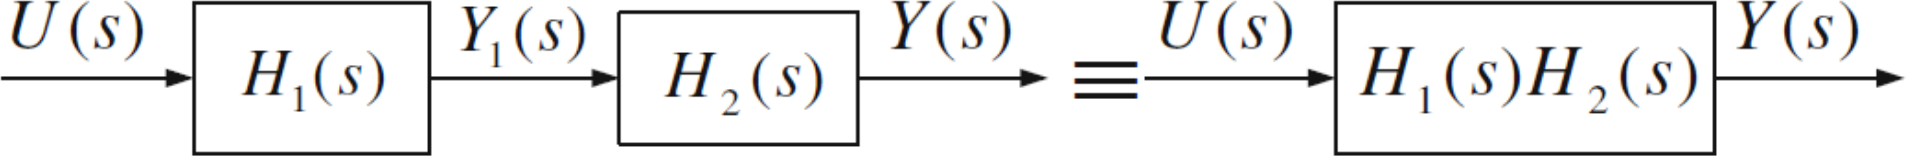
\includegraphics[\lw]{media-cheatsheet/serial.png}

\subsection{Parallel connection}
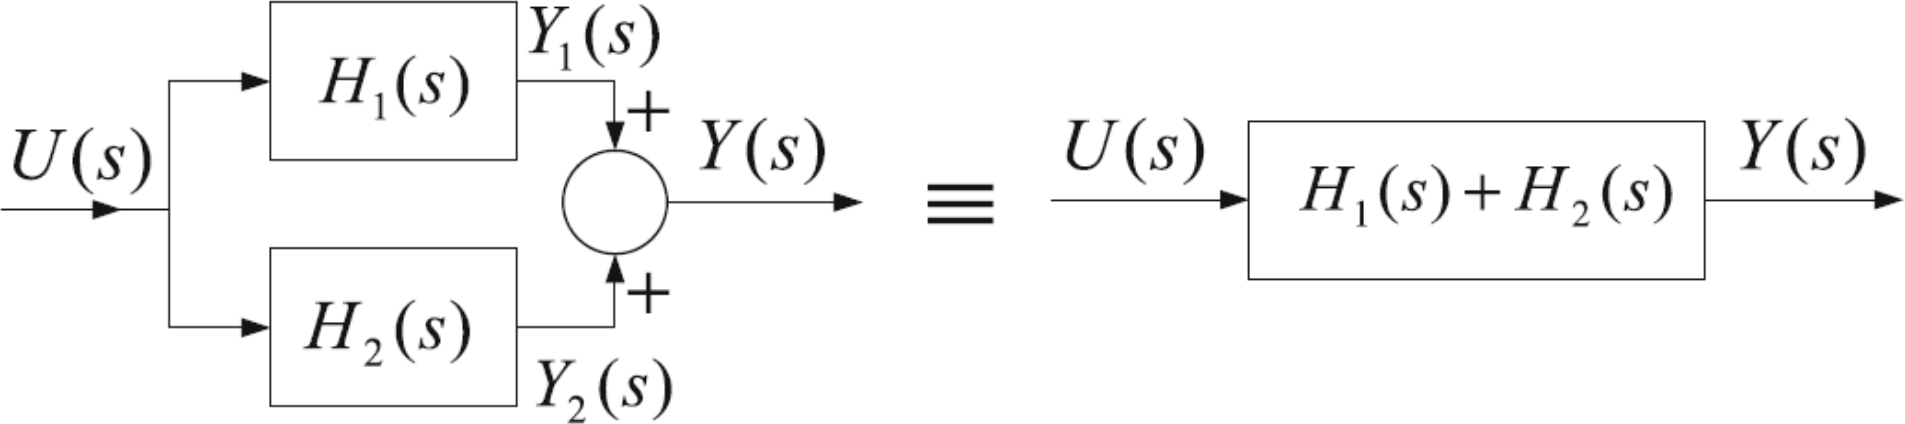
\includegraphics[\lw]{media-cheatsheet/parallel.png}

\subsection{Feedback loop 1}
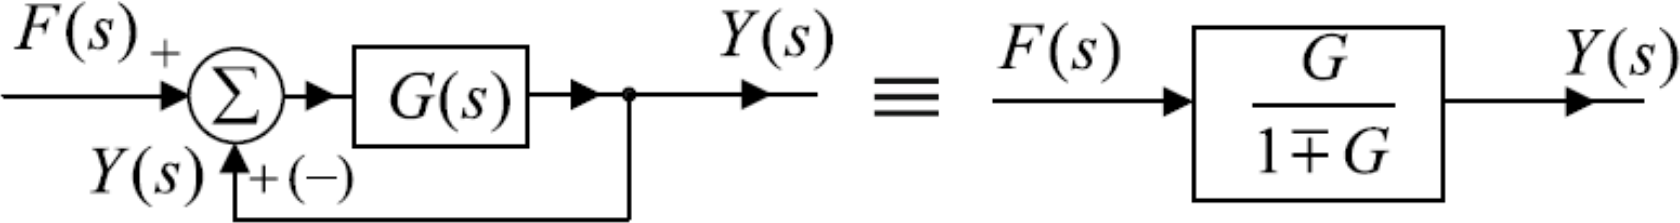
\includegraphics[\lw]{media-cheatsheet/fb1.png}

\subsection{Feedback loop 2}
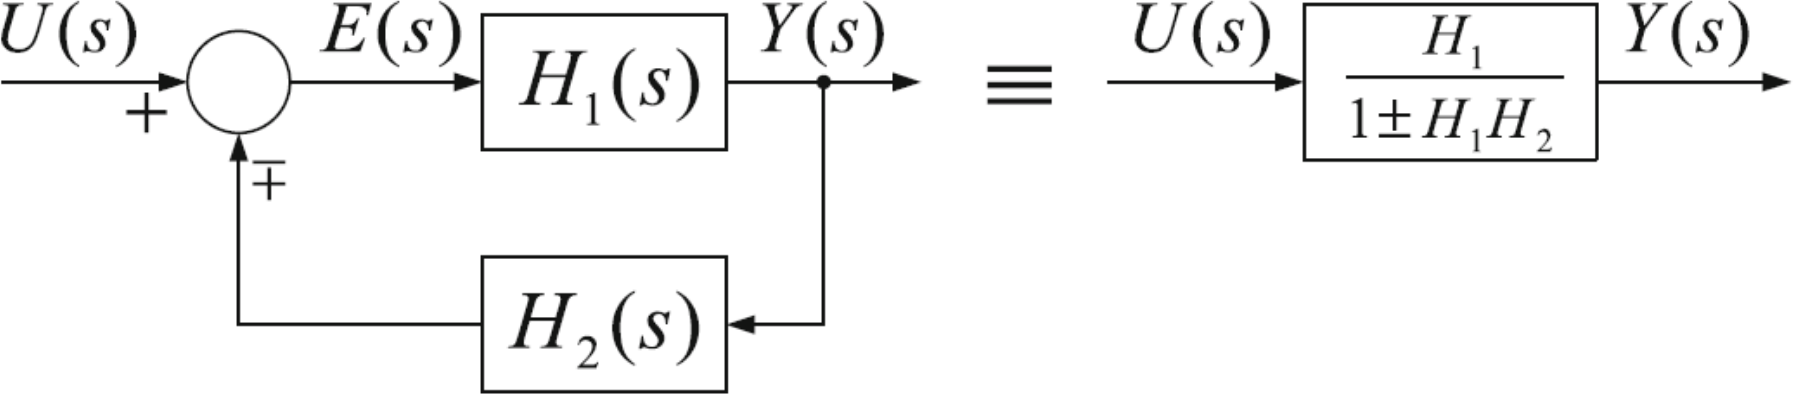
\includegraphics[\lw]{media-cheatsheet/fb2.png}

\subsection{Summation points}
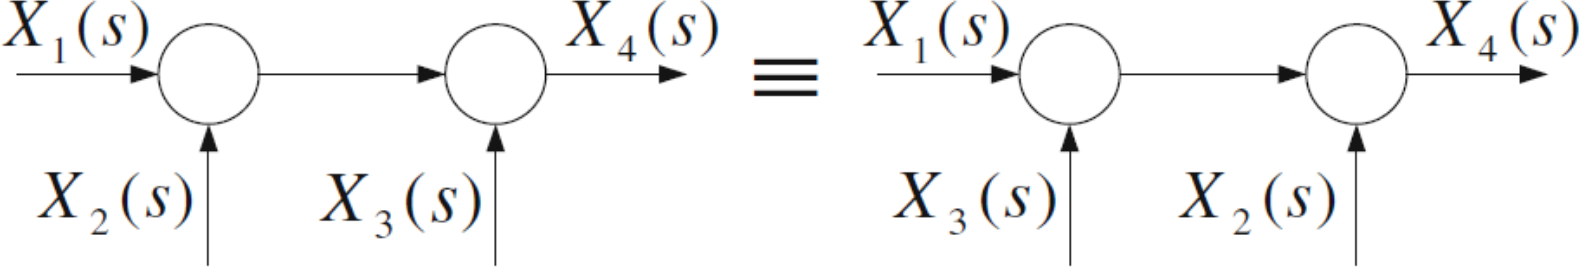
\includegraphics[\lw]{media-cheatsheet/sumpoint.png}

\subsection{Relocation of a summation 1}
\begin{center}
    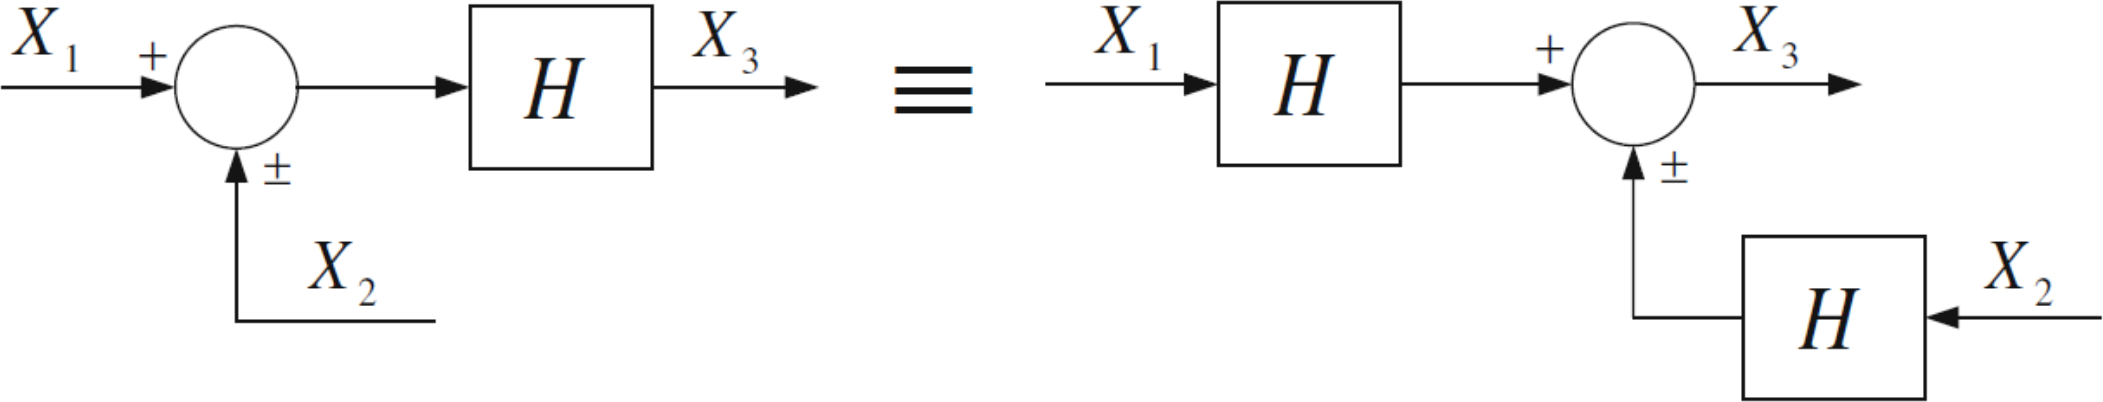
\includegraphics[\lw=.8]{media-cheatsheet/rel1.png}
\end{center}

\subsection{Relocation of a summation 2}
\begin{center}
    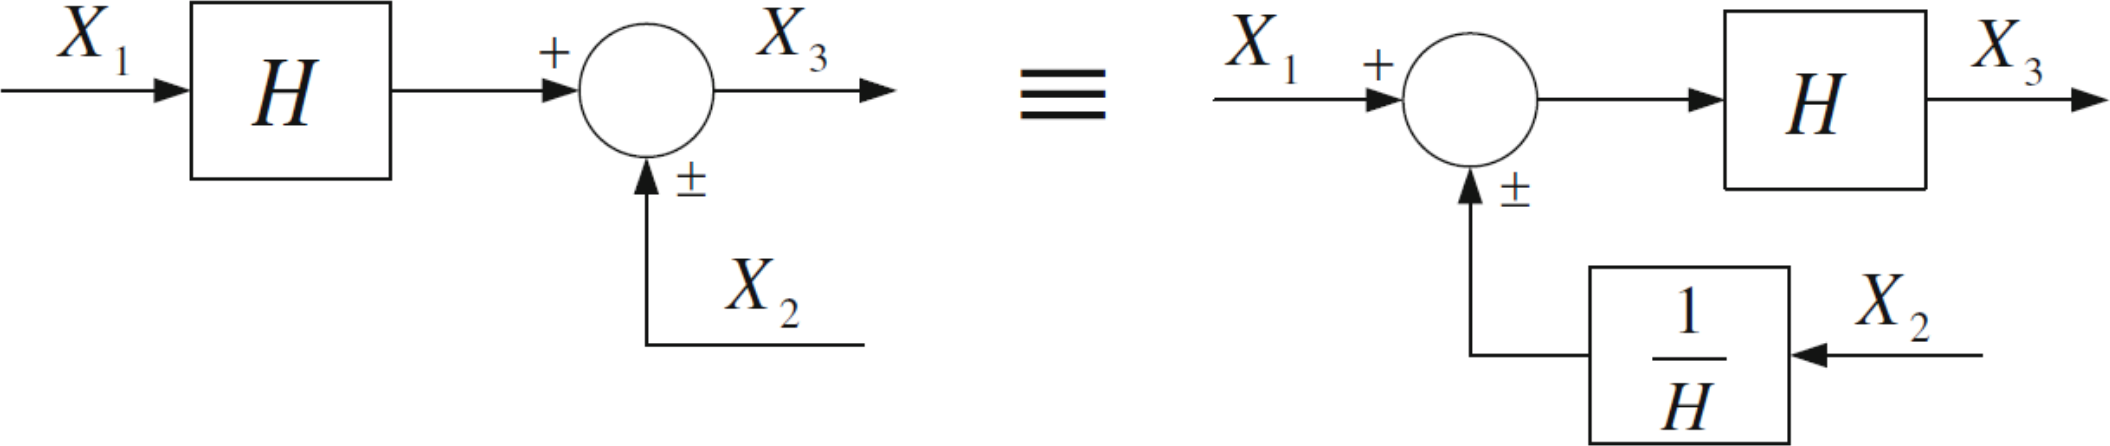
\includegraphics[\lw=.8]{media-cheatsheet/rel2.png}
\end{center}

\subsection{Relocation of a junction 1}
\begin{center}
    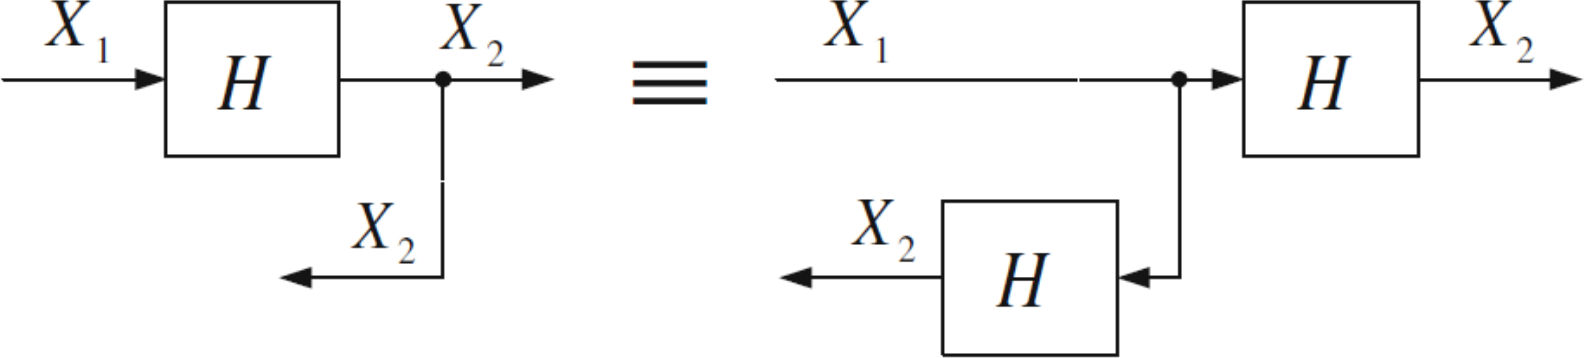
\includegraphics[\lw=.8]{media-cheatsheet/jun1.png}
\end{center}

\subsection{Relocation of a junction 2}
\begin{center}
    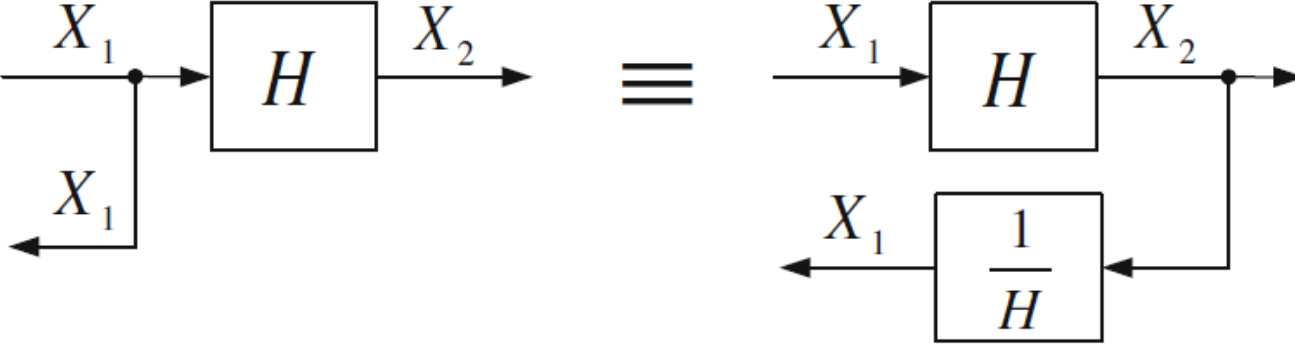
\includegraphics[\lw=.75]{media-cheatsheet/jun2.png}
\end{center}

\subsection{Relocation of a disturbance}
\begin{center}
    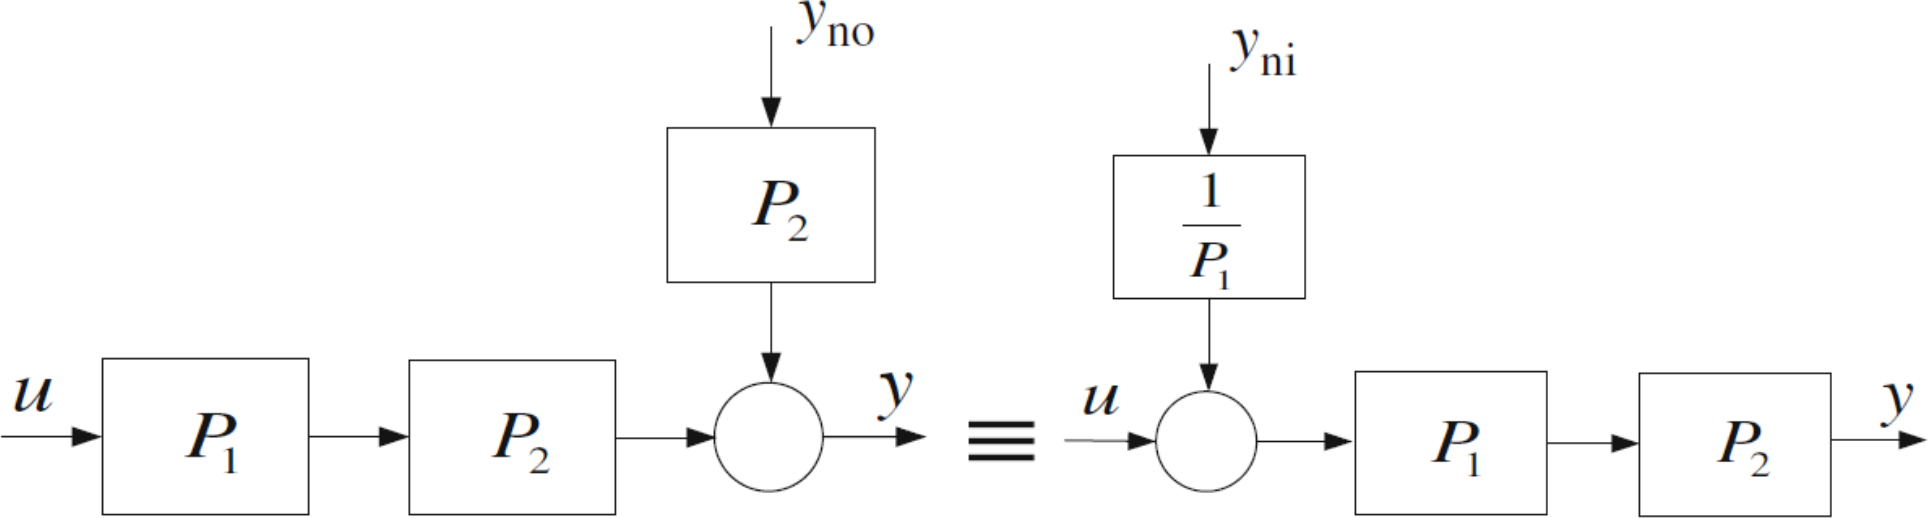
\includegraphics[\lw=.9]{media-cheatsheet/dist.png}
\end{center}

\section{Systems transfer function}
\subsection{Reference open-loop transfer function}
\begin{center}
    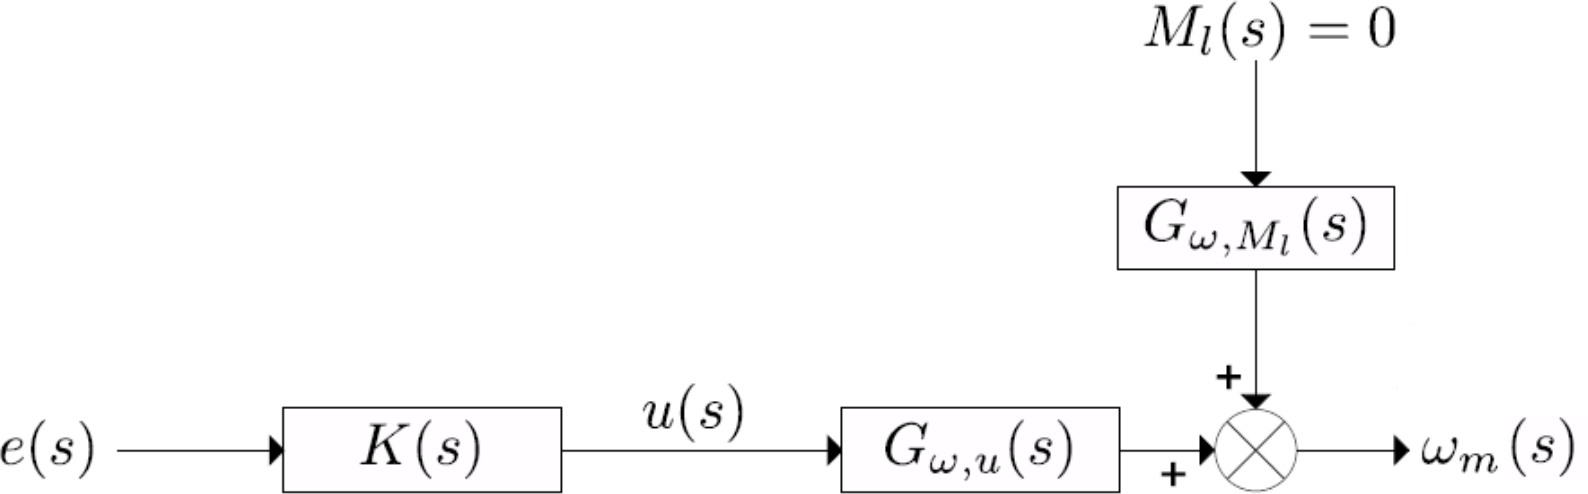
\includegraphics[\lw=.9]{media-cheatsheet/ol-tr.png}
    \[L(s) = \frac{\omega_m(s)}{e(s)} = K(s)G_{\omega,u}(s)\]
\end{center}

\subsection{Closed-loop transfer function}
\begin{center}
    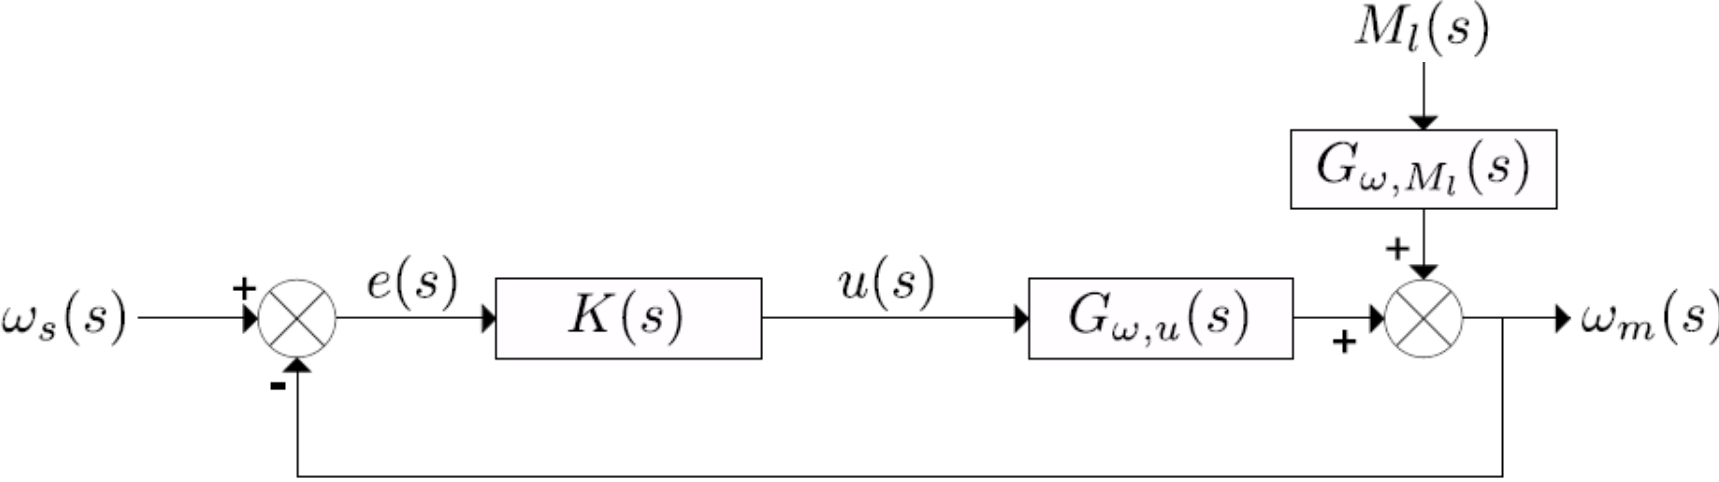
\includegraphics[\lw=.95]{media-cheatsheet/cl-tr.png}
    \begin{gather*}
    T_r(s) = \frac{\omega_m(s)}{\omega_s(s)} = \frac{K(s)G_{\omega,u}(s)}{1+K(s)G_{\omega,u}(s)}\\
    T_d(s) = \frac{\omega_m(s)}{M_l(s)} = \frac{G_{\omega,M_l}(s)}{1+K(s)G_{\omega,u}(s)}
\end{gather*}
\end{center}

\subsection{Controlled system response}
\begin{center}
    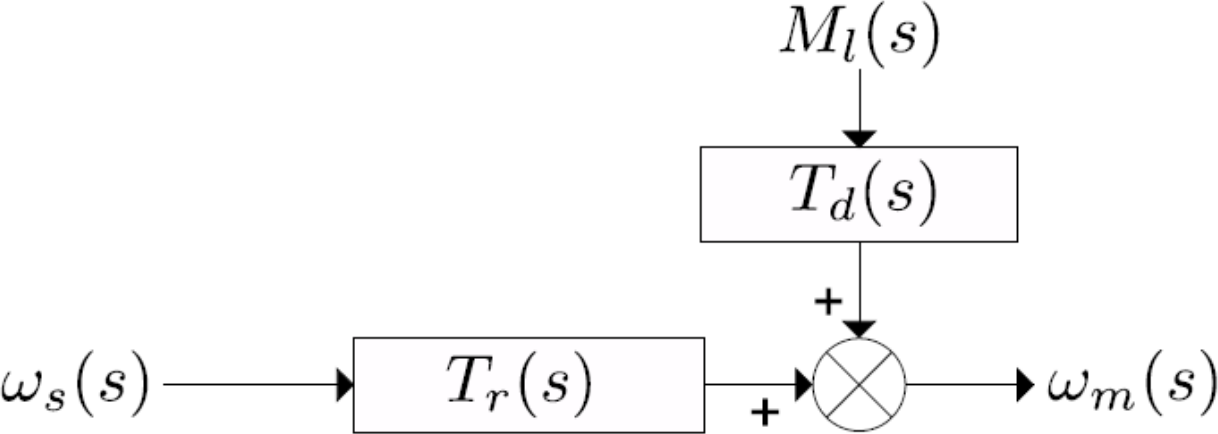
\includegraphics[\lw=.7]{media-cheatsheet/contr-tr.png}
    \[\omega_m(s) = T_r(s)\omega_s(s) + T_d(s)M_l(s)\]
\end{center}

\section{Zeros and Poles}
A system is described by its transfer function:
\[G(s)=\frac{N(s)}{D(s)}\]
\begin{itemize}
    \item Zeros: roots of $N(s)$
    \item Poles: roots of $D(s)$
\end{itemize}

\subsection{Stability}
Bounded input gives bounded output:
\[|u(t)|<\infty \Longrightarrow |y(t)|<\infty\]
Pole conditions:
\vspace*{-.2cm}
\begin{itemize}
    \item $Re<0$: stable
    \item Any $Re>0$: unstable
    \item Single pole with $Re=0$: marginally stable
    \item Repeated poles with $Re=0$: unstable
\end{itemize}

\subsection{Causality}
Output depends only on present and past inputs:
\vspace*{-.2cm}
\begin{itemize}
    \item $\deg(N)<\deg(D)$: strictly causal
    \item $\deg(N)=\deg(D)$: causal
    \item $\deg(N)>\deg(D)$: non-causal
\end{itemize}

\subsection{Oscillations}
Oscillations occur with complex poles:
\vspace*{-.2cm}
\begin{itemize}
    \item Real poles only: no oscillation
    \item $j\pm (Re=0)$: sustained oscillation
    \item $j\pm (Re<0)$: damped oscillation
    \item $j\pm (Re>0)$: increasing oscillation
\end{itemize}
\subsection{Final value theorem (steady-state)}
\[t \to \infty \stackrel{\mathcal{L}}{\Longleftrightarrow} s \to 0\quad ; \quad \boxed{\lim_{t\to\infty} y(t) = \lim_{s\to0} s\cdot Y(s)}\]
\subsubsection{Unit step final value}
\begin{gather*}
    Y(s) = G(s)U(S) = G(s)\cdot \frac{1}{s}\\
    \lim_{s\to0} s\cdot Y(s) = \lim_{s\to 0} s\cdot\frac{1}{s}\cdot G(s) = \lim_{s\to0} G(s) = G(s=0)
\end{gather*}

\subsection{Initial value theorem}
\[t \to 0 \stackrel{\mathcal{L}}{\Longleftrightarrow} s \to \infty\quad ; \quad \boxed{\lim_{t\to0} y(t) = \lim_{s\to\infty} s\cdot Y(s)}\]
\subsubsection{Unit step final value}
\begin{gather*}
    Y(s) = G(s)U(S) = G(s)\cdot \frac{1}{s}\\
    \lim_{s\to\infty} s\cdot Y(s) = \lim_{s\to\infty} s\cdot\frac{1}{s}\cdot G(s) = \lim_{s\to\infty} G(s)
\end{gather*}

\newcolumn
\vspace*{-.6cm}
\part{First- and second-order responses}
\section{Type of lag responses}
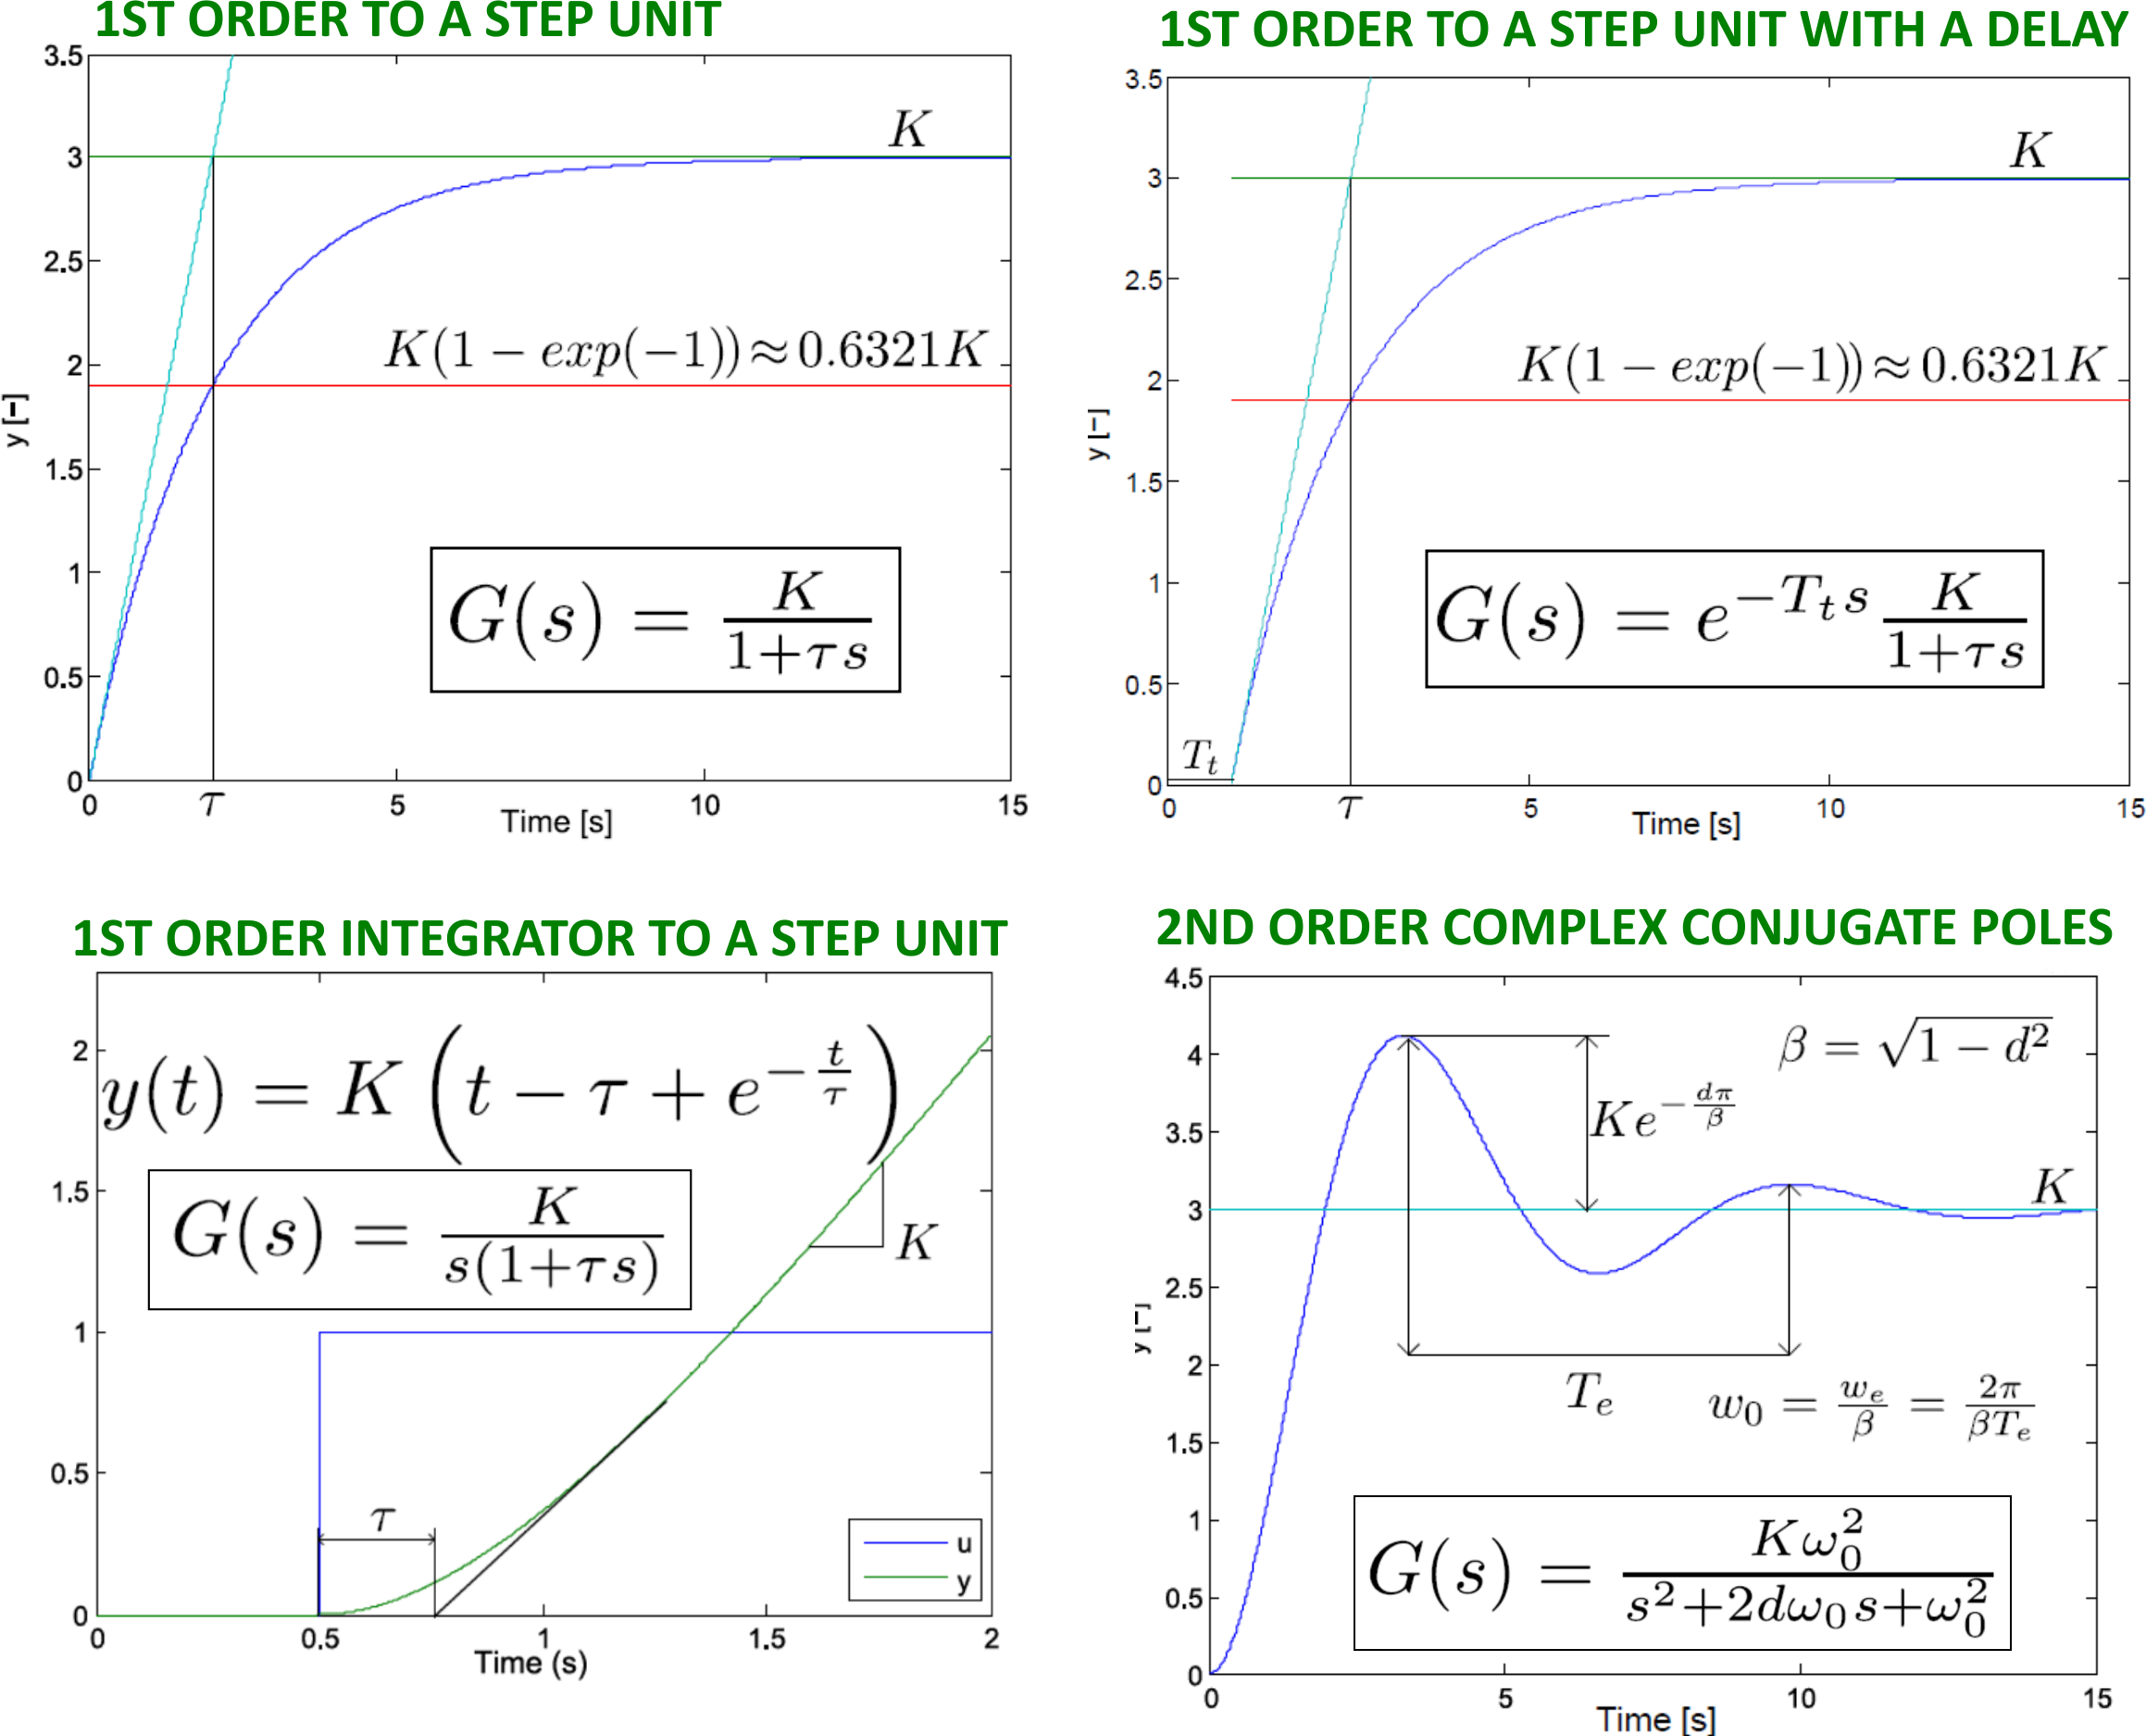
\includegraphics[\lw]{media-cheatsheet/lag-responses.png}

\part{Controller development}
\section{Kuhn method}
The process:
\[G(s) = K \frac{(1+\tau_{d,1}s)(1+\tau_{d,2}s)...(1+\tau_{d,m}s)}{(1+\tau_1 s)(1+\tau_2 s)...(1+\tau_n s)}\]
Controller parameters:
\[T_\text{sum} = T_t + \sum_{i=1}^n \tau_i - \sum_{j=1}^m \tau_{d,j}\]
\begin{center}
    \setcellgapes{2.5pt}
    \makegapedcells
    \begin{tabular}{|l|c|c|c|}
        \hline Controller type & $K_p$ & $T_i$ & $T_d$\\
        \hline PI & $\dm \frac{1}{K}$ & $0.7\cdot T_\text{sum}$ & --\\
        \hline PID & $\dm \frac{2}{K}$ & $0.8\cdot T_\text{sum}$ & $0.194\cdot T_\text{sum}$\\
        \hline 
    \end{tabular}
\end{center}

Transfer function:
\[C(s) = K_p\left(1+\frac{1}{T_i s}\right) = K_p \frac{T_i s + 1}{T_i s}\]

\newcolumn
\section{Ziegler-Nichols tuning method}
\begin{center}
    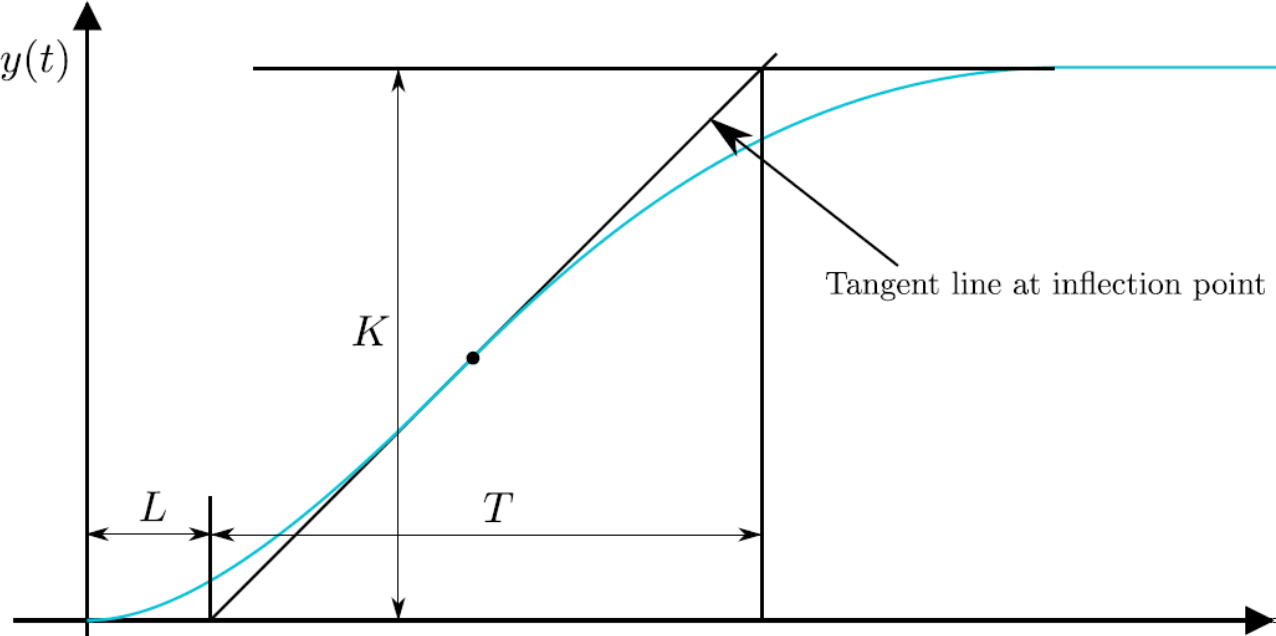
\includegraphics[\lw=.75]{media-cheatsheet/Ziegler.png}
\end{center}

First-order lag process with time delay:
\[G(s) = \frac{K}{1+\tau s}e^{-T_t s}\]

Controller parameters:
\[a = \frac{1}{K} \frac{\tau}{T_t} \quad ; \quad L = T_t\]
\begin{center}
    \setcellgapes{2.5pt}
    \makegapedcells
    \begin{tabular}{|l|c|c|c|}
        \hline Controller type & $K_p$ & $T_i$ & $T_d$\\
        \hline P & $a$ & -- & --\\
        \hline PI & $0.9\cdot a$ & $3\cdot L$ & -- \\
        \hline PID & $1.2\cdot a$ & $2\cdot L$ & $0.5\cdot L$\\
        \hline 
    \end{tabular}
\end{center}

Transfer function:
\begin{gather*}
\text{P:}\quad C(s) = K_p = a \\[6pt]
\text{PI:}\quad C(s) = K_p\left(1+\frac{1}{T_i s}\right)
= 0.9\cdot a\left(1+\frac{1}{3Ls}\right)
= 0.9\cdot a \frac{3Ls+1}{3Ls} \\[6pt]
\text{PID:}\quad C(s) = K_p\left(1+\frac{1}{T_i s}+T_d s\right)
= 1.2\cdot a\left(1+\frac{1}{2Ls}+0.5Ls\right)
= 1.2\cdot a \frac{L^2s^2+2Ls+1}{2Ls}
\end{gather*}

\newpage
\section{True/False}
\scriptsize
\begin{enumerate}[leftmargin=*, itemsep=2pt, parsep=1pt]
    \item Time discretization is called sampling. \textbf{\textcolor{darkgreen}{T}}
    \item From a system-modelling point of view, springs and capacitors are analogous as elements in mechanical and electrical systems, respectively. \textbf{\textcolor{darkgreen}{T}}
    \item A stable system must exhibit a bounded/limited output for a bounded/limited input. \textbf{\textcolor{darkgreen}{T}}
    \item Feedback control systems can feed sensor noise into the system. \textbf{\textcolor{darkgreen}{T}}
    \item The integral is represented by $s$ in the s-domain. \textbf{\textcolor{red}{F}}; integration is represented by $\frac{1}{s}$.
    \item A system modelled by $\ddot{y}(t)+\dot{y}(t)=u(t)$ is time-variant. \textbf{\textcolor{red}{F}}; it is time-invariant.
    \item Two first-order systems in series result in a second-order system. \textbf{\textcolor{darkgreen}{T}}
    \item High damping coefficient results in oscillatory response of a second-order system. \textbf{\textcolor{red}{F}}; low damping causes oscillations.
    \item Adding a real derivative action (D) to a PI controller strongly decreases oscillations, as well as overshoots. \textbf{\textcolor{darkgreen}{T}}
    \item In a PID controller, an increase in the derivative gain affects the steady-state error. \textbf{\textcolor{red}{F}}; steady-state error is mainly affected by integral action.
    \item A process modelled by $3\dot{y}(t)-4y^3(t)=2u(t)$ is linear. \textbf{\textcolor{red}{F}}
    \item A process modelled by $y(t)=t^2x(t)$ is stable. \textbf{\textcolor{red}{F}}; a bounded input can give an unbounded output.
    \item While actuators, sensors and physical processes are in the lowest level of the automation pyramid, the top level represents business management. \textbf{\textcolor{darkgreen}{T}}
    \item A parallel combination of two systems represented by $A(s)$ and $B(s)$ results in $H(s)=A(s)\cdot B(s)$. \textbf{\textcolor{red}{F}}; parallel transfer functions add.
    \item The command signal of controller $C$ is equal to $C(e(t))$, with $e(t)$ being the tracking error. \textbf{\textcolor{darkgreen}{T}}
    \item First-order systems typically exhibit faster responses than comparable higher-order systems. \textbf{\textcolor{darkgreen}{T}}
    \item Feedforward can be used to improve reference tracking and disturbance rejection abilities of a system. \textbf{\textcolor{darkgreen}{T}}
    \item Two complex conjugate poles lead to an oscillating behavior of systems. \textbf{\textcolor{darkgreen}{T}}
    \item The Laplace transform of the delta function (unit impulse) is $\frac{1}{s}$. \textbf{\textcolor{red}{F}}; $\mathcal{L}\{\delta(t)\}=1$.
    \item The ODE diagram can be drawn for non-linear processes. \textbf{\textcolor{darkgreen}{T}}
    \item A process modelled by $\dot{y}(t)=y(t)+u(t)$ is unstable. \textbf{\textcolor{darkgreen}{T}}
    \item A process is stable if all poles of its transfer function have negative real parts. \textbf{\textcolor{darkgreen}{T}}
    \item The step answer of a first-order lag oscillates. \textbf{\textcolor{red}{F}}
    \item The ODE diagram can be drawn for a non-linear process. \textbf{\textcolor{darkgreen}{T}}
    \item Nowadays, most controllers are implemented in a digital way. \textbf{\textcolor{darkgreen}{T}}
    \item An instable process can be stabilized with an open-loop controller. \textbf{\textcolor{red}{F}}
    \item A good disturbance rejection behavior means that the tracking error is small for reference signals of interest. \textbf{\textcolor{red}{F}}; this describes reference tracking.
    \item Two complex conjugate poles lead to an oscillating behavior. \textbf{\textcolor{darkgreen}{T}}
    \item A process, stable when uncontrolled, remains necessarily stable once closed-loop controlled for any controller. \textbf{\textcolor{red}{F}}
    \item An integrator is needed in a controller to improve the steady-state behavior. \textbf{\textcolor{darkgreen}{T}}
    \item Measurement noises are amplified by the derivative component of a controller. \textbf{\textcolor{darkgreen}{T}}
    \item An integrator is good to make an unstable process stable. \textbf{\textcolor{red}{F}}
    \item A simple household bread toaster is an example of an open-loop control system. \textbf{\textcolor{darkgreen}{T}}
    \item Sensors deliver accurate measurement data of the process output and do not possess any internal noise or inaccuracies. \textbf{\textcolor{red}{F}}
    \item Systems are the physical carriers of information in communication, measurement, and control processes. \textbf{\textcolor{red}{F}}; signals are the information carriers.
    \item The automation pyramid represents the hierarchical structure of industrial automation systems, from field levels at the bottom to enterprise levels at the top. \textbf{\textcolor{darkgreen}{T}}
    \item Feedforward can be used to improve reference tracking and disturbance rejection abilities of a system. \textbf{\textcolor{darkgreen}{T}}
    \item A process modelled by $\dot{y}(t)-3y^2(t)-2u(t)=0$ is linear. \textbf{\textcolor{red}{F}}
    \item A process modelled by $2\dot{y}(t)-\sqrt{3}y(t)=\ln(2)\cdot u(t)$ is linear. \textbf{\textcolor{darkgreen}{T}}
    \item The unit ramp signal is the first derivative of the unit step signal. \textbf{\textcolor{red}{F}}; the derivative of the ramp is the step.
    \item Derivation in the time domain is represented by $\frac{1}{s}$ in the Laplace domain. \textbf{\textcolor{red}{F}}; differentiation is represented by $s$.
    \item Sampling an analog signal leads to time discretization. \textbf{\textcolor{darkgreen}{T}}
    \item Digitalization involves sampling in time and quantization of the amplitude. \textbf{\textcolor{darkgreen}{T}}
    \item Integration in the time domain is represented by $s$ in the Laplace domain. \textbf{\textcolor{red}{F}}; integration is represented by $\frac{1}{s}$.
    \item The output of a linear, time-invariant system with impulse response $h(t)$ to an input $x(t)$ is represented in the Laplace domain by $Y(s)=X(s)\cdot H(s)$. \textbf{\textcolor{darkgreen}{T}}
    \item A parallel combination of two systems represented by $A(s)$ and $B(s)$ results in $H(s)=A(s)\cdot B(s)$. \textbf{\textcolor{red}{F}}; parallel transfer functions add.
    \item If $H(s)$ were the system transfer function, then $\lim_{s\to 0}H(s)$ would represent the steady-state behavior of the system. \textbf{\textcolor{darkgreen}{T}}
    \item Two complex conjugate poles lead to an oscillating behavior of systems. \textbf{\textcolor{darkgreen}{T}}
\end{enumerate}

\section{Components of a medical infusion pump system}
\tiny
\textbf{Reference signal / setpoint}\\
Set / desired concentration of medication in the patient's bloodstream, set by the nurse. It
specifies the desired concentration of medication that the infusion pump system aims to
maintain, as prescribed by the healthcare provider.

\textbf{Controller}\\
Infusion Pump System. It monitors the measured concentration of medication in the patient's
bloodstream and adjusts the infusion rate to maintain the set concentration. The controller
acts as the controller in the closed-loop system. It compares the measured medication
concentration (feedback) with the set concentration (reference signal) and adjusts the
infusion rate accordingly to maintain the desired concentration.

\textbf{Process}\\
Infusion Pump, i.e., the physical system (infusion pump) that delivers the medication into
the patient's bloodstream based on the control signal from the infusion pump system. The
process represents the physical mechanism (infusion pump) that controls the flow rate of
medication into the patient's bloodstream based on the control signal from the infusion pump
system.

\textbf{Process output}\\
Patient's current medication concentration. That is, the actual concentration of medication in
the patient's bloodstream, continuously monitored and compared to the set concentration.
The actual output of the controlled system is the concentration of medication in the patient's
bloodstream. This output is continuously monitored and compared to the set concentration.

\textbf{Disturbances}\\
Factors such as changes in patient's metabolism, variations in blood flow, or external factors
affecting medication absorption. Disturbances are external and internal factors that can
affect the medication concentration in the patient's bloodstream, influencing the
effectiveness of treatment.

\textbf{Feedback signal}\\
Measured medication concentration. That is, the actual concentration of medication in the
patient's bloodstream, measured by sensors and fed back to the infusion pump system to
adjust the infusion rate. The actual concentration of medication in the patient's bloodstream
is measured, providing real-time feedback to the infusion pump system to adjust the infusion
rate in response to changes.

\section{Laplace transform}
Derive $F(s)$ of the following time-domain signal:
\begin{gather*}
    f(t) = \dfrac{1}{4}e^{-5t}\cdot u(t)\\
    F(s) = \integral[0][\infty][f(t)e^{-st}][t] = \integral[0][\infty][\dfrac{1}{4}e^{-5t}\cdot u(t)e^{-st}][t]\\
    \dfrac{1}{4}\integral[0][\infty][e^{-(5+s)t}][t] = \dfrac{1}{4}\left[\dfrac{e^{-(5+s)t}}{-(5+s)}\right]_0^\infty\\
    \dfrac{-1}{4(5+s)}\left[0-1\right] = \dfrac{1}{4(5+s)},\ \forall Re\{s\} > -5
\end{gather*}

\section{Closed-loop controller}
\footnotesize
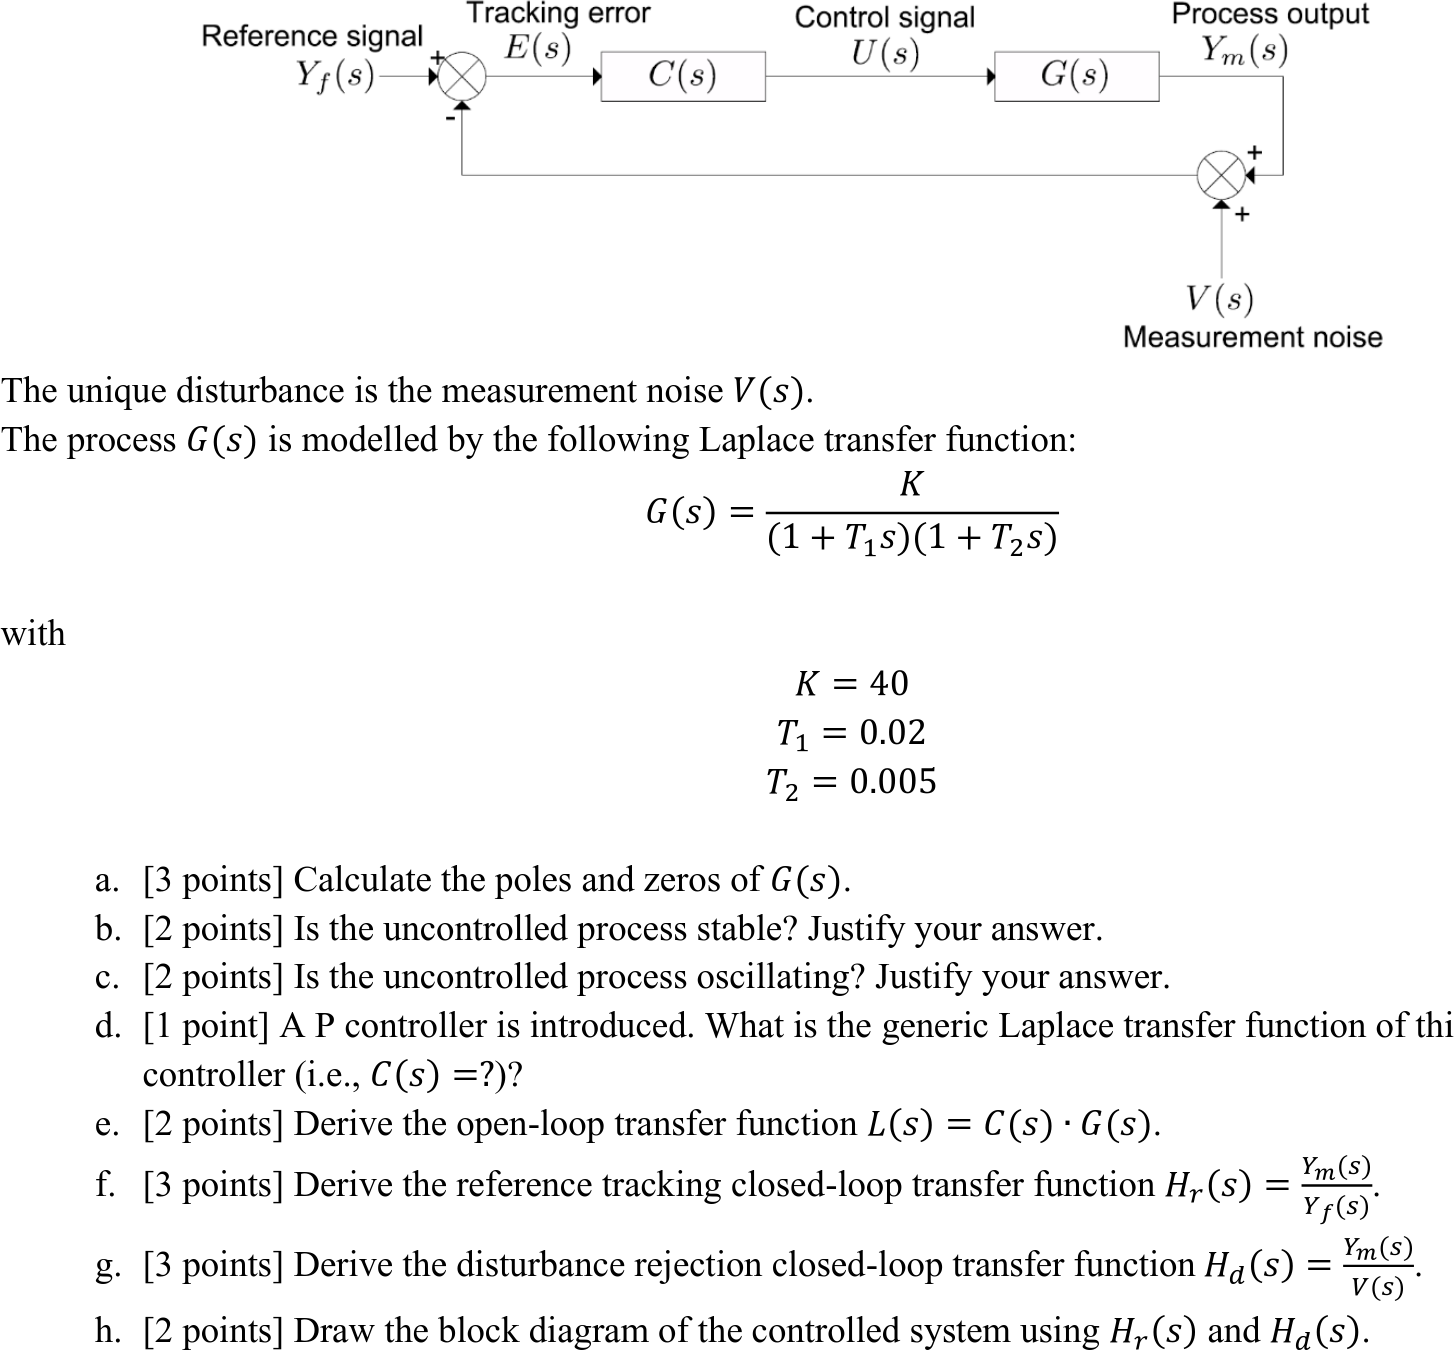
\includegraphics[\lw]{media-cheatsheet/ex.png}
\begin{enumerate}[label=\alph*.]
    \item Zeros: $G(s) = 0 \Rightarrow$ no zeros\\
        Poles: $(1+T_1s)(1+T_2s) = 0 \Rightarrow s_1 = \dfrac{-1}{T_1} = -50;\ s_2 = \dfrac{-1}{T_2} = -200$
    \item Stable, because the real-part of all poles are negative
    \item No. There are no complex-conjugate poles
    \item $C(s) = K_p$
    \item $L(s) = C(s)G(s) = K_p\dfrac{K}{(1+T_1s)(1+T_2s)} = \dfrac{40 K_p}{10^{-4}s^2 + 0.025s + 1}$\\[0.5ex]
    \item $H_r(s) = \dfrac{L(s)}{1+L(s)} = \dfrac{\frac{40K_p}{20^{-4}s^2+0.025s+1}}{1+\frac{40K_p}{10^{-4}s^2+0.025s+1}} = \dfrac{40K_p}{10^{-4}s^2+0.025s+1+40K_p}$\\[0.5ex]
    \item $H_d(s) = L(s)\cdot\left[-v(s)-Y_m(s)\right] \Rightarrow Y_m(s)\left[1+L(s)\right] = -v(s)L(s)$\\
        $\Rightarrow \dfrac{-L(s)}{1+L(s)} = \dfrac{-40K_p}{10^{-4}s^2+0.025s+1+40K_p}$
    \item \begin{minipage}{0.48\linewidth}
        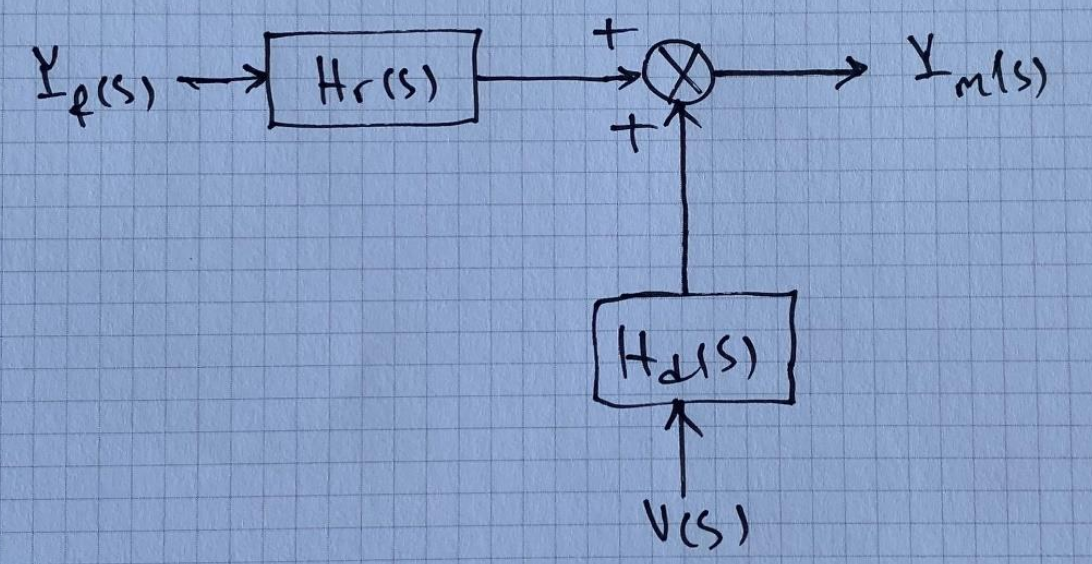
\includegraphics[width=\linewidth]{media-cheatsheet/bl1.png}
    \end{minipage}
    \begin{minipage}{0.48\linewidth}
        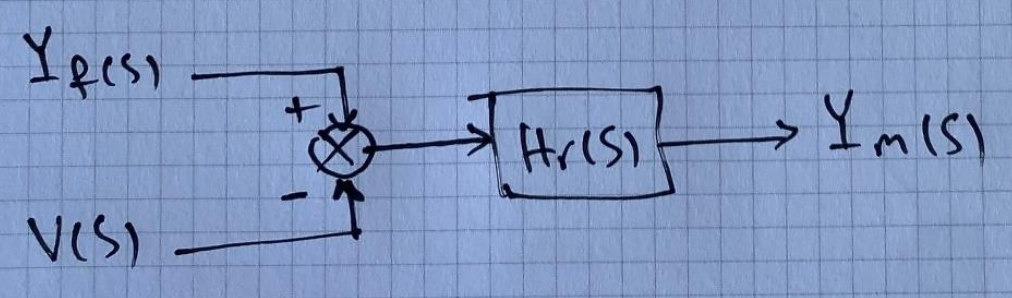
\includegraphics[width=\linewidth]{media-cheatsheet/bl2.png}
    \end{minipage}
\end{enumerate}

\subsection{Closed-loop block diagram example}
\begin{center}
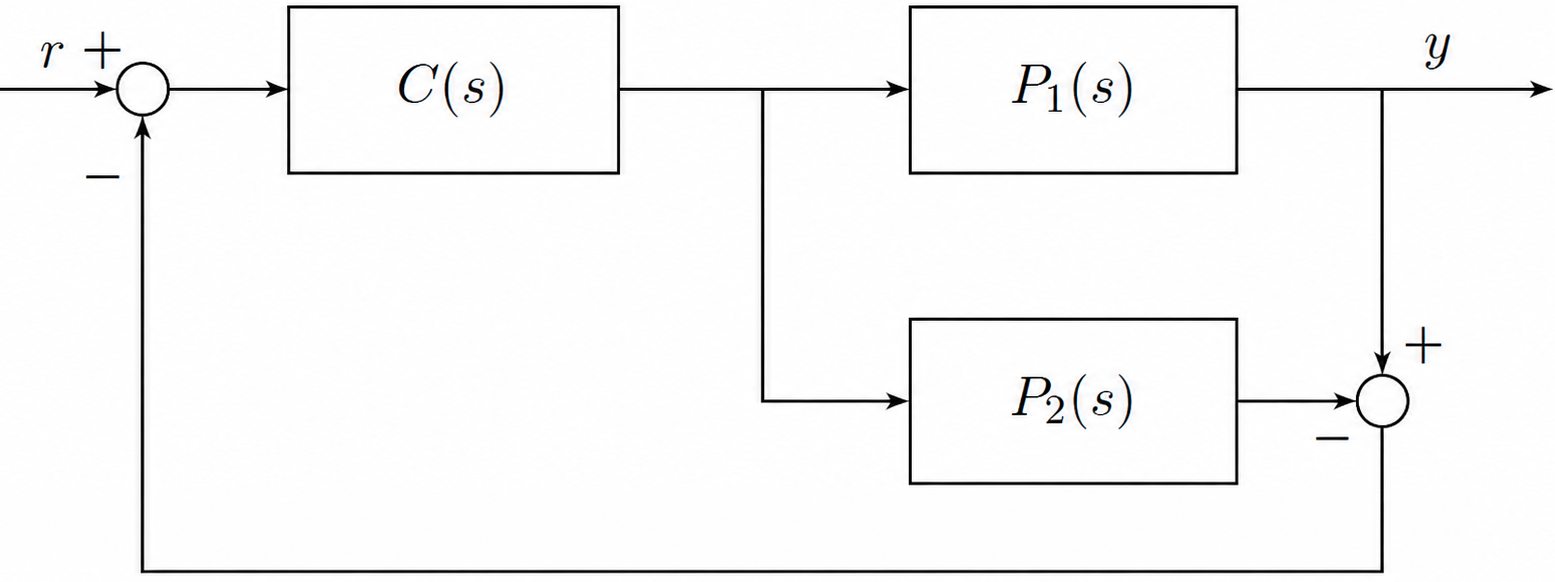
\includegraphics[\lw=.7]{media-cheatsheet/ex_hs22.png}
\end{center}
With $P_1(s)=\dfrac{3}{s-1}$, $P_2(s)=\dfrac{1}{s-1}$ and $C(s)=2$,
calculate the transfer function $G(s) = \frac{Y(s)}{R(s)}$
\begin{gather*}
    u(s) = C(s)e(s),\qquad Y(s)=P_1(s)u(s)\\
    e(s)=R(s)-\left(P_1(s)u(s)-P_2(s)u(s)\right)
    =R(s)-\left(P_1(s)-P_2(s)\right)C(s)e(s)\\
    e(s)\left[1+C(s)\left(P_1(s)-P_2(s)\right)\right]=R(s)\\
    G(s)=\frac{Y(s)}{R(s)}
    =\frac{C(s)P_1(s)}{1+C(s)\left(P_1(s)-P_2(s)\right)}\\
    =\frac{2\cdot\frac{3}{s-1}}{1+2\left(\frac{3}{s-1}-\frac{1}{s-1}\right)}
    =\frac{\frac{6}{s-1}}{\frac{s+3}{s-1}}
    =\boxed{\frac{6}{s+3}}
\end{gather*}

\subsection{Steady-state error from block diagram}
Question: find the smallest positive $k_p$ such that the unity-feedback system is
stable and, for a unit step $r(t)$, $\lim_{t\to\infty}|e(t)|\le 0.1$.
\begin{center}
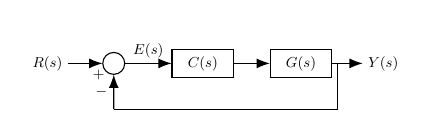
\begin{tikzpicture}[>=Latex, scale=0.58, every node/.style={transform shape}]
    \node (r) at (0,0) {$R(s)$};
    \node[draw, circle, inner sep=1.2pt, minimum size=0.48cm] (sum) at (1.45,0) {};
    \node[draw, minimum width=1.35cm, minimum height=0.62cm] (c) at (3.4,0) {$C(s)$};
    \node[draw, minimum width=1.35cm, minimum height=0.62cm] (g) at (5.55,0) {$G(s)$};
    \node (y) at (7.35,0) {$Y(s)$};
    \draw[->] (r) -- (sum);
    \draw[->] (sum) -- node[above] {$E(s)$} (c);
    \draw[->] (c) -- (g);
    \draw[->] (g) -- (y);
    \draw (6.35,0) |- (1.45,-1.0);
    \draw[->] (1.45,-1.0) -- (sum);
    \node at (1.12,-0.25) {$+$};
    \node at (1.18,-0.62) {$-$};
\end{tikzpicture}
\end{center}
\[
    C(s)=k_p,\qquad G(s)=\frac{1}{1+10s}
\]
Unity negative feedback:
\begin{gather*}
    E(s)=R(s)-Y(s),\qquad Y(s)=C(s)G(s)E(s)\\
    E(s)=\frac{R(s)}{1+C(s)G(s)}
    =\frac{R(s)(1+10s)}{1+10s+k_p}
\end{gather*}
For a unit step $R(s)=\frac{1}{s}$:
\begin{gather*}
    e_\infty=\lim_{t\to\infty}e(t)
    =\lim_{s\to0}sE(s)
    =\frac{1}{1+k_p}\\
    \left|e_\infty\right|\le 0.1
    \Rightarrow \frac{1}{1+k_p}\le 0.1
    \Rightarrow k_p\ge 9
\end{gather*}
Closed-loop pole:
\[
    1+10s+k_p=0 \Rightarrow s=-\frac{1+k_p}{10}
\]
Stable for $k_p>-1$, therefore the smallest positive gain satisfying both conditions is
\[
    \boxed{k_p=9}
\]

\subsection{Order and free integrator from step response}
Proportional-control negative feedback, unit step input. The open-loop transfer
function $L(s)$ is stated to be 2nd order and without zeros.
\begin{center}
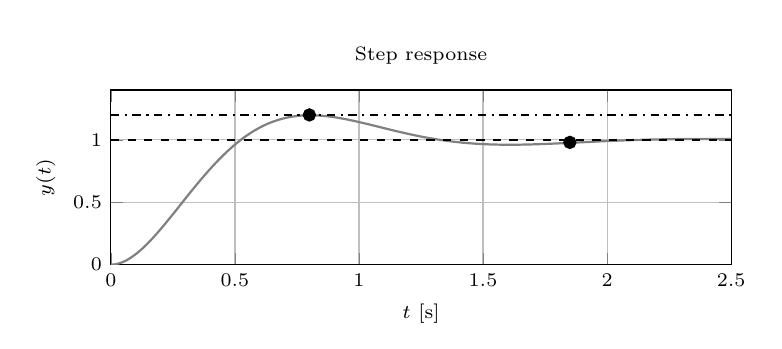
\begin{tikzpicture}
    \begin{axis}[
        width=.78\linewidth,
        height=3.8cm,
        xmin=0, xmax=2.5,
        ymin=0, ymax=1.4,
        xlabel={$t$ [s]},
        ylabel={$y(t)$},
        title={Step response},
        grid=both,
        tick label style={font=\scriptsize},
        label style={font=\scriptsize},
        title style={font=\scriptsize},
        legend style={font=\scriptsize, draw=none},
        every axis plot/.append style={line width=0.8pt}
    ]
        \addplot[gray, domain=0:2.5, samples=160]
        {1 - exp(-2.02*x)*(cos(deg(3.91*x)) + 0.516*sin(deg(3.91*x)))};
        \addplot[dashed] coordinates {(0,1) (2.5,1)};
        \addplot[dash dot] coordinates {(0,1.2) (2.5,1.2)};
        \addplot[only marks, mark=*] coordinates {(0.8,1.2) (1.85,0.98)};
    \end{axis}
\end{tikzpicture}
\end{center}
\textbf{a) Question:} Use the graph to give two arguments that $L(s)$ is at
least 2nd order.
\begin{itemize}
    \item Overshoot and damped oscillation imply complex conjugate closed-loop poles.
    A 1st order system cannot oscillate or overshoot without zeros.
    \item The response starts with zero initial slope, which is typical for a
    strictly proper system with relative degree $\ge 2$.
\end{itemize}
\textbf{b) Question:} Does the graph justify that $L(s)$ contains a free
integrator?
\[
    T(s)=\frac{Y(s)}{R(s)}=\frac{L(s)}{1+L(s)},\qquad
    y_\infty=T(0)
\]
The graph settles at $y_\infty\approx 1$ for a unit step, so the steady-state
error is approximately zero:
\[
    e_\infty=1-y_\infty\approx 0
\]
For unity negative feedback this requires $L(0)\to\infty$, which is obtained
when $L(s)$ contains a free integrator:
\[
    \boxed{L(s)\ \text{contains a free integrator}}
\]

\subsection{Closed loop with measurement noise}
\tiny
Question: solve the following closed-loop process with measurement noise
$V(s)$, process $G(s)$, and controller $C(s)$.
\begin{center}
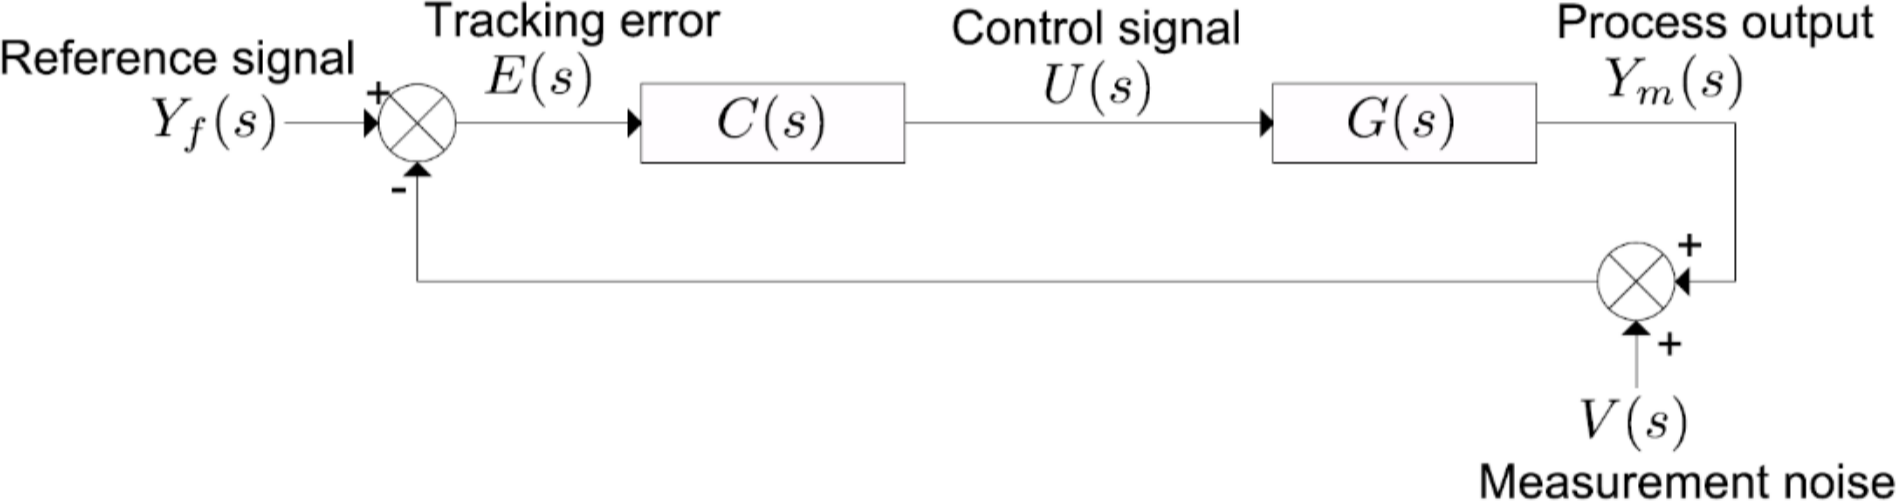
\includegraphics[\lw=.8]{media-cheatsheet/ex22-2.png}
\end{center}
\[
    G(s)=\frac{K}{(1+T_1s)(1+T_2s)},\qquad
    K=30,\ T_1=0.01,\ T_2=0.001
\]
\begin{enumerate}[label=\alph*.]
    \item \textbf{Calculate the poles and zeros of $G(s)$.}\\
    No zeros.\\
    Poles: $1+T_1s=0,\ 1+T_2s=0 \Rightarrow
    \boxed{s_1=-100,\ s_2=-1000}$.
    \item \textbf{Is this process stable? Justify.}\\
    Stable, because all poles have negative real part.
    \item \textbf{A P controller is introduced. What is its generic transfer function?}\\
    \[
        \boxed{C(s)=k_p}
    \]
    \item \textbf{Derive the open-loop transfer function $L(s)$.}
    \[
        \boxed{L(s)=C(s)G(s)
        =\frac{30k_p}{(1+0.01s)(1+0.001s)}
        =\frac{30k_p}{10^{-5}s^2+0.011s+1}}
    \]
    \item \textbf{Derive the reference tracking closed-loop transfer function.}\\
    With $V=0$:
    \[
        \boxed{\frac{Y_m(s)}{Y_f(s)}=\frac{L(s)}{1+L(s)}
        =\frac{30k_p}{10^{-5}s^2+0.011s+1+30k_p}}
    \]
    \item \textbf{Derive the disturbance rejection closed-loop transfer function.}\\
    With $Y_f=0$:
    \[
        E(s)=Y_f(s)-Y_m(s)-V(s),\quad Y_m(s)=L(s)E(s)
    \]
    \[
        \boxed{\frac{Y_m(s)}{V(s)}=-\frac{L(s)}{1+L(s)}
        =-\frac{30k_p}{10^{-5}s^2+0.011s+1+30k_p}}
    \]
    \item \textbf{Calculate the steady-state error as a function of $k_p$.}\\
    Unit-step reference and $V=0$:
    \[
        e_\infty=\lim_{s\to0}sE(s)
        =\frac{1}{1+L(0)}
        =\boxed{\frac{1}{1+30k_p}}
    \]
    \item \textbf{Which values of $k_p$ lead to a steady-state error smaller than $5\%$?}
    \[
        \left|\frac{1}{1+30k_p}\right|<0.05
        \quad\text{and stable }(k_p>-1/30)
        \Rightarrow \boxed{k_p>\frac{19}{30}\approx0.633}
    \]
    \item \textbf{A PID controller is introduced. What is its generic transfer function?}
    \[
        \boxed{C(s)=k_p\left(1+\frac{1}{T_is}+T_ds\right)}
    \]
    \item \textbf{Choose $T_i$ and $T_d$ so that $L(s)$ simplifies to
    $\frac{KK_p}{T_is}$.}\\
    Given $C(s)=K_p(1+T_ds)\frac{1+T_is}{T_is}$, choose
    \[
        \boxed{T_i=T_1=0.01,\qquad T_d=T_2=0.001}
    \]
    so that
    \[
        L(s)=C(s)G(s)
        =K_p(1+T_2s)\frac{1+T_1s}{T_1s}
        \frac{K}{(1+T_1s)(1+T_2s)}
        =\boxed{\frac{KK_p}{T_is}}
    \]
    \item \textbf{Derive the reference closed-loop transfer function using these
    parameters; $k_p$ is free.}
    \[
        \boxed{\frac{Y_m(s)}{Y_f(s)}
        =\frac{\frac{KK_p}{T_is}}{1+\frac{KK_p}{T_is}}
        =\frac{KK_p}{T_is+KK_p}
        =\frac{30K_p}{0.01s+30K_p}}
    \]
    \item \textbf{Derive the disturbance rejection closed-loop transfer function.}
    \[
        \boxed{\frac{Y_m(s)}{V(s)}
        =-\frac{\frac{KK_p}{T_is}}{1+\frac{KK_p}{T_is}}
        =-\frac{KK_p}{T_is+KK_p}
        =-\frac{30K_p}{0.01s+30K_p}}
    \]
    \item \textbf{Calculate the steady-state error with this new controller.}\\
    With the PID, the free integrator gives
    \[
        e_\infty=\frac{1}{1+L(0)}=\boxed{0}
    \]
\end{enumerate}

\subsection{Equivalent block diagram}
\footnotesize
Question: the two systems are equivalent. Write $H(s)$ as a function of $C(s)$
and $G(s)$, reporting the algebraic steps.
\begin{center}
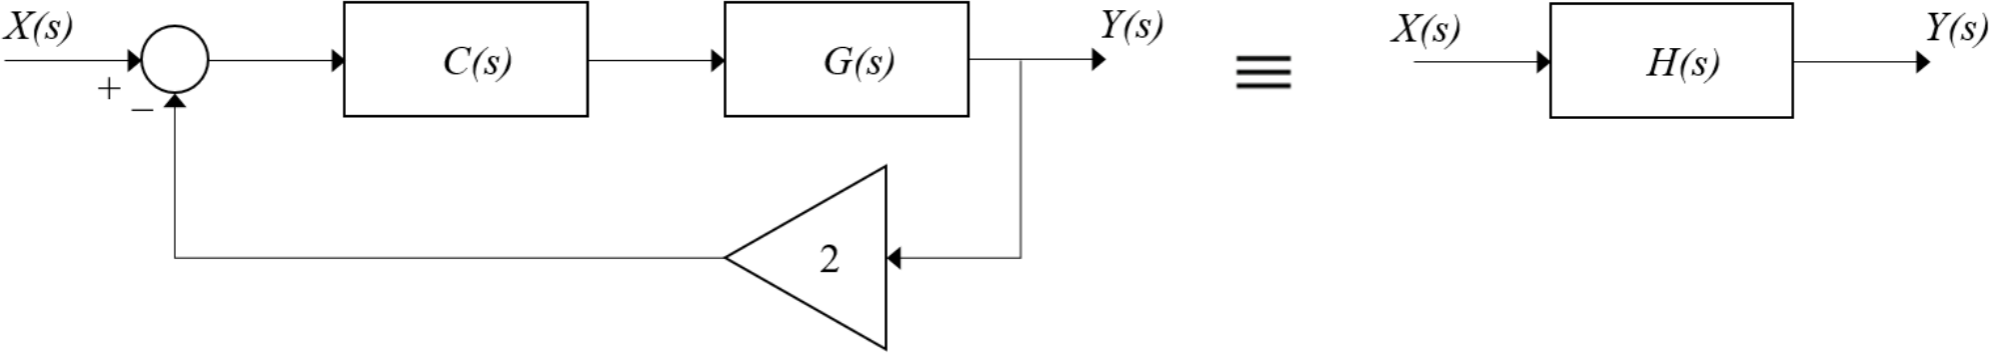
\includegraphics[\lw]{media-cheatsheet/ex-21-1.png}
\end{center}
Let the summing-junction output be $E(s)$. The feedback signal is $2Y(s)$:
\begin{gather*}
    E(s)=X(s)-2Y(s)\\
    Y(s)=C(s)G(s)E(s)
    =C(s)G(s)\left[X(s)-2Y(s)\right]\\
    Y(s)=C(s)G(s)X(s)-2C(s)G(s)Y(s)\\
    Y(s)\left[1+2C(s)G(s)\right]=C(s)G(s)X(s)
\end{gather*}
Therefore
\[
    H(s)=\frac{Y(s)}{X(s)}
    =\boxed{\frac{C(s)G(s)}{1+2C(s)G(s)}}
\]

\subsection{First-order process with PI controller}
Question: a process is modelled by
\[
    G(s)=\frac{Y(s)}{X(s)}=\frac{50}{1+0.2s}.
\]
\begin{enumerate}[label=\alph*.]
    \item \textbf{Derive the differential equation corresponding to $G(s)$.}
    \[
        \frac{Y(s)}{X(s)}=\frac{50}{1+0.2s}
        \Rightarrow (1+0.2s)Y(s)=50X(s)
    \]
    \[
        \boxed{y(t)+0.2\dot{y}(t)=50x(t)}
    \]
    \item \textbf{Draw a block diagram for this process.}
    \begin{center}
    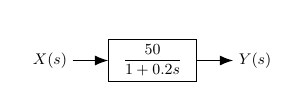
\begin{tikzpicture}[>=Latex, scale=0.62, every node/.style={transform shape}]
        \node (x) at (0,0) {$X(s)$};
        \node[draw, minimum width=1.8cm, minimum height=0.65cm] (g) at (2.1,0)
        {$\dfrac{50}{1+0.2s}$};
        \node (y) at (4.2,0) {$Y(s)$};
        \draw[->] (x) -- (g);
        \draw[->] (g) -- (y);
    \end{tikzpicture}
    \end{center}
    \item \textbf{Determine the orders of numerator and denominator of $G(s)$.}
    \[
        \boxed{\deg N(s)=0,\qquad \deg D(s)=1}
    \]
    \item \textbf{Compute the poles and zeros of this transfer function.}\\
    No zeros. Pole:
    \[
        1+0.2s=0 \Rightarrow \boxed{s=-5}
    \]
    \item \textbf{Is this process stable? Explain.}\\
    Yes. The only pole is in the left half-plane: $s=-5<0$.
    \item \textbf{The controller is
    $C(s)=0.02\frac{1+0.2s}{s}$. What kind of controller is this?}
    \[
        C(s)=0.02\frac{1+0.2s}{s}
        =0.004\frac{1+0.2s}{0.2s}
        =0.004\left(1+\frac{1}{0.2s}\right)
    \]
    \[
        \boxed{\text{PI controller with }k_p=0.004,\ T_i=0.2}
    \]
    \item \textbf{Derive the open-loop transfer function $L(s)$.}
    \[
        L(s)=C(s)G(s)
        =0.02\frac{1+0.2s}{s}\cdot\frac{50}{1+0.2s}
        =\boxed{\frac{1}{s}}
    \]
    \item \textbf{Derive the reference tracking closed-loop transfer function.}
    \[
        \boxed{\frac{Y(s)}{R(s)}
        =\frac{L(s)}{1+L(s)}
        =\frac{\frac{1}{s}}{1+\frac{1}{s}}
        =\frac{1}{s+1}}
    \]
    \item \textbf{Compute the steady-state error for a unit-step input.}
    \[
        E(s)=\frac{R(s)}{1+L(s)}
        =\frac{\frac{1}{s}}{1+\frac{1}{s}}
        =\frac{1}{s+1}
    \]
    \[
        e_\infty=\lim_{s\to0}sE(s)=\boxed{0}
    \]
    \item \textbf{Draw the step answer for a unit-step input.}\\
    Since $\frac{Y(s)}{R(s)}=\frac{1}{s+1}$ and $R(s)=\frac{1}{s}$:
    \[
        Y(s)=\frac{1}{s(s+1)}
        \Rightarrow \boxed{y(t)=1-e^{-t}}
    \]
    \begin{center}
    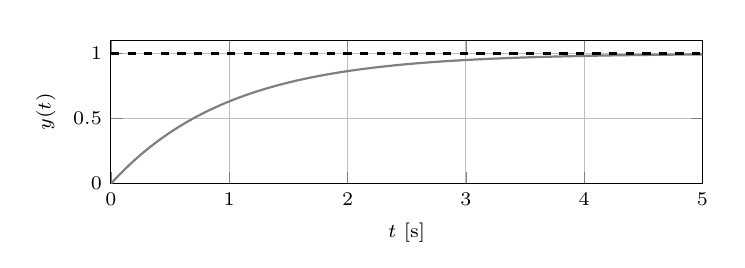
\begin{tikzpicture}
        \begin{axis}[
            width=.75\linewidth,
            height=3.4cm,
            xmin=0, xmax=5,
            ymin=0, ymax=1.1,
            xlabel={$t$ [s]},
            ylabel={$y(t)$},
            grid=both,
            tick label style={font=\scriptsize},
            label style={font=\scriptsize},
            every axis plot/.append style={line width=0.8pt}
        ]
            \addplot[gray, domain=0:5, samples=120] {1-exp(-x)};
            \addplot[dashed] coordinates {(0,1) (5,1)};
        \end{axis}
    \end{tikzpicture}
    \end{center}
\end{enumerate}

\subsection{First-order lag answer computation}
Question: a process can be modelled by
\[
    G(s)=\frac{Y(s)}{U(s)}=\frac{100}{0.1s+1}.
\]
\begin{enumerate}[label=\alph*.]
    \item \textbf{Derive the differential equation corresponding to $G(s)$.}
    \[
        \frac{Y(s)}{U(s)}=\frac{100}{0.1s+1}
        \Rightarrow (0.1s+1)Y(s)=100U(s)
    \]
    \[
        \boxed{0.1\dot{y}(t)+y(t)=100u(t)}
    \]
    \item \textbf{Compute the poles and zeros of this transfer function.}\\
    No zeros. Pole:
    \[
        0.1s+1=0 \Rightarrow \boxed{s=-10}
    \]
    \item \textbf{Is this process stable?}\\
    Yes. The only pole is in the left half-plane: $s=-10<0$.
    \item \textbf{Draw the step answer of this process for a step with amplitude 1.}
    \[
        Y(s)=G(s)\frac{1}{s}
        =\frac{100}{s(0.1s+1)}
        \Rightarrow \boxed{y(t)=100\left(1-e^{-10t}\right)}
    \]
    \begin{center}
    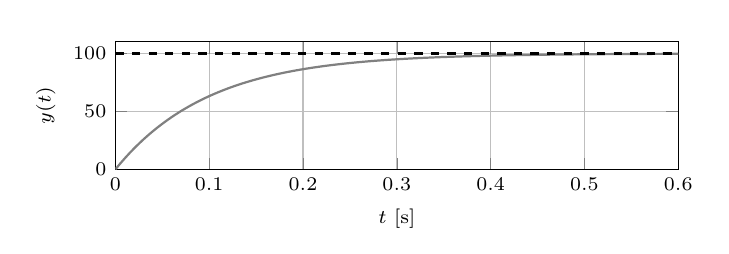
\begin{tikzpicture}
        \begin{axis}[
            width=.72\linewidth,
            height=3.2cm,
            xmin=0, xmax=0.6,
            ymin=0, ymax=110,
            xlabel={$t$ [s]},
            ylabel={$y(t)$},
            grid=both,
            tick label style={font=\scriptsize},
            label style={font=\scriptsize},
            every axis plot/.append style={line width=0.8pt}
        ]
            \addplot[gray, domain=0:0.6, samples=120] {100*(1-exp(-10*x))};
            \addplot[dashed] coordinates {(0,100) (0.6,100)};
        \end{axis}
    \end{tikzpicture}
    \end{center}
    \item \textbf{Draw the step answer of this process for a step with amplitude 2.}
    \[
        Y(s)=G(s)\frac{2}{s}
        =\frac{200}{s(0.1s+1)}
        \Rightarrow \boxed{y(t)=200\left(1-e^{-10t}\right)}
    \]
    \begin{center}
    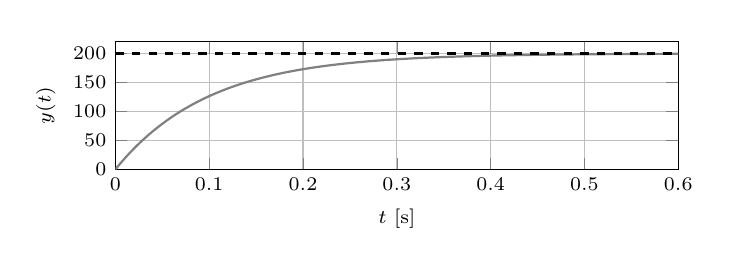
\begin{tikzpicture}
        \begin{axis}[
            width=.72\linewidth,
            height=3.2cm,
            xmin=0, xmax=0.6,
            ymin=0, ymax=220,
            xlabel={$t$ [s]},
            ylabel={$y(t)$},
            grid=both,
            tick label style={font=\scriptsize},
            label style={font=\scriptsize},
            every axis plot/.append style={line width=0.8pt}
        ]
            \addplot[gray, domain=0:0.6, samples=120] {200*(1-exp(-10*x))};
            \addplot[dashed] coordinates {(0,200) (0.6,200)};
        \end{axis}
    \end{tikzpicture}
    \end{center}
    \item \textbf{The controller is
    $C(s)=0.01\frac{0.1s+1}{s}$. What kind of controller is that?}
    \[
        C(s)=0.01\frac{0.1s+1}{s}
        =0.001\frac{0.1s+1}{0.1s}
        =0.001\left(1+\frac{1}{0.1s}\right)
    \]
    \[
        \boxed{\text{PI controller with }k_p=0.001,\ T_i=0.1}
    \]
    \item \textbf{Derive the open-loop transfer function $L(s)$.}
    \[
        L(s)=C(s)G(s)
        =0.01\frac{0.1s+1}{s}\cdot\frac{100}{0.1s+1}
        =\boxed{\frac{1}{s}}
    \]
    \item \textbf{Derive the reference tracking closed-loop transfer function.}
    \[
        \boxed{\frac{Y(s)}{R(s)}
        =\frac{L(s)}{1+L(s)}
        =\frac{\frac{1}{s}}{1+\frac{1}{s}}
        =\frac{1}{s+1}}
    \]
    \item \textbf{Compute the steady state error.}
    \[
        E(s)=\frac{R(s)}{1+L(s)}
        =\frac{\frac{1}{s}}{1+\frac{1}{s}}
        =\frac{1}{s+1}
    \]
    \[
        \boxed{e_\infty=\lim_{s\to0}sE(s)=0}
    \]
    \item \textbf{Draw the process output if the reference signal is a step with amplitude 1.}
    \[
        Y(s)=\frac{1}{s+1}\cdot\frac{1}{s}
        =\frac{1}{s(s+1)}
        \Rightarrow \boxed{y(t)=1-e^{-t}}
    \]
    \begin{center}
    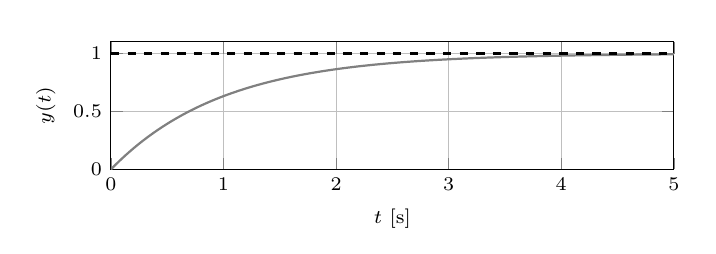
\begin{tikzpicture}
        \begin{axis}[
            width=.72\linewidth,
            height=3.2cm,
            xmin=0, xmax=5,
            ymin=0, ymax=1.1,
            xlabel={$t$ [s]},
            ylabel={$y(t)$},
            grid=both,
            tick label style={font=\scriptsize},
            label style={font=\scriptsize},
            every axis plot/.append style={line width=0.8pt}
        ]
            \addplot[gray, domain=0:5, samples=120] {1-exp(-x)};
            \addplot[dashed] coordinates {(0,1) (5,1)};
        \end{axis}
    \end{tikzpicture}
    \end{center}
\end{enumerate}

\end{multicols*}

\end{document}
